\documentclass{book}




\usepackage{fullpage}
\usepackage{amsmath}
\usepackage{amsfonts}
\usepackage{amsthm}
\usepackage{graphicx}
\usepackage{framed}
\usepackage{algorithmic}
\usepackage{xcolor}

\definecolor{dark_red}{rgb}{0.5,0.0,0.0}
\definecolor{dark_green}{rgb}{0.0,0.5,0.0}
\definecolor{dark_blue}{rgb}{0.0,0.0,0.5}
\definecolor{red}{rgb}{1.0,0.0,0.0}
\definecolor{blue}{rgb}{0.0,0.0,1.0}

\newcommand{\dr}[1]{\textcolor{dark_red}{#1}}
\newcommand{\dg}[1]{\textcolor{dark_green}{#1}}
\newcommand{\db}[1]{\textcolor{dark_blue}{#1}}
\newcommand{\red}[1]{\textcolor{red}{#1}}
\newcommand{\blue}[1]{\textcolor{blue}{#1}}

\newtheorem{lma}{Lemma}
\newtheorem{thm}{Theorem}
\newtheorem{cor}{Corollary}

\title{An Intuitive and Visual Approach to Vector Calculus and Electromagnetism}
\author{Shawn Eastwood}
\date{}

\begin{document}

\frontmatter

\maketitle


\chapter*{Introduction}

\addcontentsline{toc}{chapter}{Introduction}

Many discussions and introductions to vector calculus utilize examples and proofs that are exercises in symbolic computation. It is of this author's opinion that a symbolic approach to vector calculus does not convey core concepts in a sufficiently clear manner. Abstract proofs, abstract formulas, and examples for which the emphasis is on the algebra and symbolic computation do not convey the core essence of vector calculus.  

The primary purpose of this document is to provide an introduction to vector calculus and electromagnetism {\bf without using the language of Calculus}. The material presented below will use easy to visualize concepts and keep equations and numbers to a minimum. Any equation given will be accompanied by a high level description that will make such equations intuitive. 

The primary application that will be presented will be electromagnetism and Maxwell's equations. Most approaches to electromagnetism are piece-wise. For example, basic circuit analysis is primarily concerned with voltages, currents, and resistances. Eventually inductance and mutual inductance is introduced. What is rarely mentioned in these discussions is that the electric field is not conservative, and therefore the notion of voltage itself is poorly defined. While the magnetic vector potential can be used to ``complete" the electric field and create a field that is conservative, the vector potential itself is not uniquely defined and is subject to multiple ``gauges". Within inductors in particular, the voltage difference across the inductor is in direct opposition to the electric field that actually exists. The voltage difference is instead the electric field that must exist to ``push back" the electric field generated by the inductor itself.

%Perfect current itself does not actually exist: current is the movement of point charges, mostly electrons. With the a more accurate picture of current, Maxwell's equations will be modified to a more accurate picture where the movement of field lines, not electric

The aim is to enable a visualization of electromagnetic phenomena that takes full account of Maxwell's equations. To this end, conventional depictions of vector fields as a forest of arrows will be replaced in favor of depictions that use bundles of oriented paths and layers of oriented surfaces. Using terminology from fluid mechanics, the description will be {\bf Lagrangian} in nature as opposed to more conventional {\bf Eulerian} descriptions. With Eulerian descriptions, the fields are tracked at {\bf fixed points}. With the Lagrangian description, the field lines will be tracked as they sweep through space. 

\section*{What will be assumed}

This document will assume that the reader is familiar with basic algebra. 

While a basic knowledge of Calculus is useful, an in-depth knowledge of Calculus is not required. 

Since the conventional depiction of vectors as arrows is being replaced, vector algebra is also not required as a prerequisite topic. When vectors are introduced, they will be introduced as lists of numbers.

\section*{Chapter structure}

Chapter 1 introduces the fundamental structures of points, paths, surfaces, and volumes. Chapters 2 to 4 introduce the basic functions involving points, paths, surfaces, and volumes. Chapters 5 and 6 establish algebraic properties involving the introduced structures and operations. 

Chapter 7 introduces the system by which points, paths, surfaces, and volumes can be quantified directly with numbers and functions. It is in this chapter that a prior knowledge of differential calculus is useful. 

Chapter 8 describes how the dimensionality of structures can be ``inverted", with points becoming volumes and vice versa, and with paths becoming surfaces and vice versa. It is at this point that electromagnetism is introduced assuming no changes with respect to time (i.e. statics). Many important details related to electrostatics and magnetostatics will be proven. 

Chapter 9 finally introduces time. Additional functions are introduced. The computations from chapter 7 and the concept of duality from chapter 8 are extended to incorporate time.

Chapter 10 finally fully introduces electromagnetism with the incorporation of time.  

Chapter 11 connects electromagnetism with force, momentum, and energy. 


\tableofcontents




\mainmatter


\chapter{Multi-structures}

\section{Introduction}

This chapter will introduce the structures that will serve as the basis for all of the concepts that will be discussed by this book. 

A \textbf{multi-structure} is a collection of points (a multi-point), a collection of paths (a multi-path), a collection of surfaces (a multi-surface), or a collection of volumes (a multi-volume). The ``type" of a multi-structure is the status of being a multi-point, a multi-path, a multi-surface, or a multi-volume. All of these structures will be assumed to exist in {\bf 3D space}.


\section{Multi-points}

~

\begin{tabular}{cc}
\parbox{0.5\textwidth}{
A \textbf{multi-point} is a superposition of points. One such superposition is depicted on the right.
} & \parbox{0.5\textwidth}{
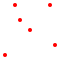
\includegraphics[scale = 0.75]{Multi-structures/Multipoints/multi-point_simple}
}
\end{tabular}

\vspace{5mm}

\begin{tabular}{cc}
\parbox{0.5\textwidth}{
When two points have the same position, the result is a point with a weight of \(2\). When three points have the same position, the result is a point with a weight of \(3\). Every point in a multi-point has associated with it a ``weight" which is the number of how many points have been stacked into the same position. The weight can be a fraction, so there can be fractional copies of a point. The weight can also be negative, so there can be ``anti-points". If the weight is \(0\), then the point is simply not included. On the right is a multi-point, where the points have different weights.
} & \parbox{0.5\textwidth}{
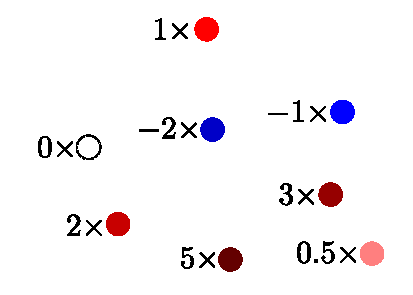
\includegraphics[scale = 0.75]{Multi-structures/Multipoints/multi-point_multiplicity}
}
\end{tabular}

\vspace{2mm}

A multi-point \(\rho\) is effectively a set of point (\(P\)) / weight (\(w\)) pairs. An arbitrary multi-point will be denoted via the notation
\[\rho = w_1 P_1 + w_2 P_2 + ... + w_N P_N\]
where \(w_i\) is the weight that is assigned to point \(P_i\). This notation effectively denotes that a multi-point is a collection/sum of points.

Each weight \(w_i\) will be assumed to be nonzero, as a point with a weight of 0 is not included as part of the multi-point. Moreover, the points will be assumed to all be unique. If a point appears multiple times, then these appearances can be condensed into a single appearance whose weight is the sum of all weights from the multiple appearances. 




\section{Multi-paths}

A path is 1D trail. An oriented path is a path that has a preferred direction as is depicted in the four examples below:
\begin{center}
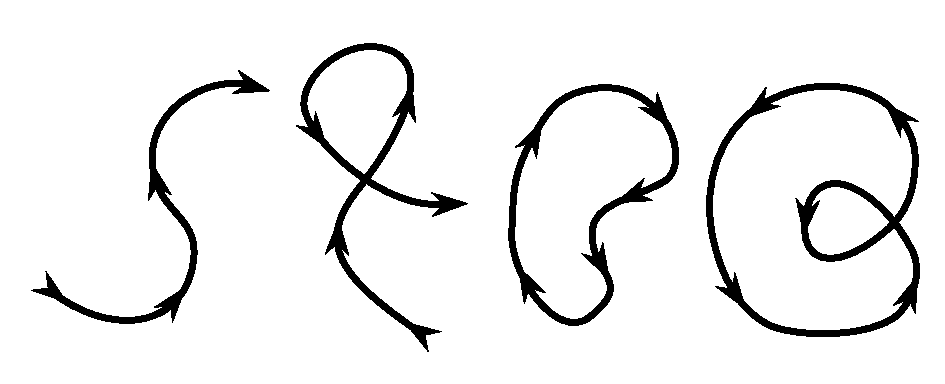
\includegraphics[scale = 0.5]{Multi-structures/Multipaths/oriented_paths}
\end{center}

\begin{tabular}{cc}
\parbox{0.5\textwidth}{
A \textbf{multi-path} is a superposition of oriented paths. One such superposition is depicted on the right.
} & \parbox{0.5\textwidth}{
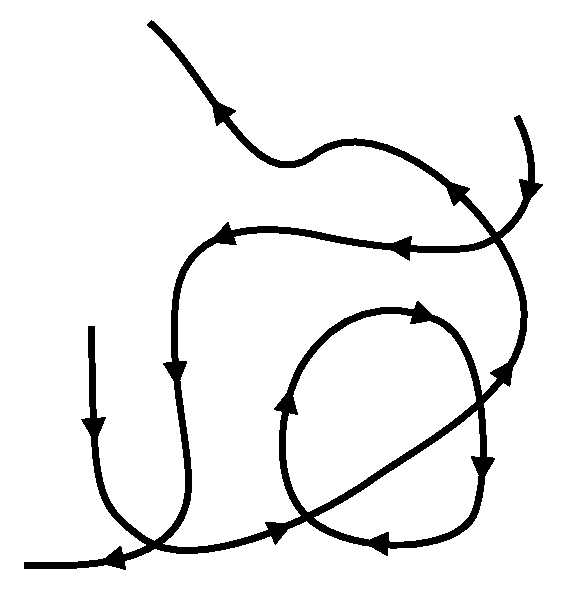
\includegraphics[scale = 0.7]{Multi-structures/Multipaths/multi-path_simple}
}
\end{tabular}

\begin{tabular}{cc}
\parbox{0.5\textwidth}{
When two oriented paths in the same multi-path are equivalent, the result is the common oriented path with a weight of \(2\). When three oriented paths in the same multi-path are the equivalent, the result is the common oriented path with a weight of \(3\). Every oriented path in a multi-path has associated with it a ``weight" which is the number of ``stacked" oriented paths. The weight can be a fraction, so there can be fractional copies of a path. {\bf If the weight is negative, then the orientation of the path is reversed and the sign is flipped to positive.} On the right is a multi-path where the paths have different weights. Note how there are no negative weights, as a negative weight merely flips the orientation of the path.  
} & \parbox{0.5\textwidth}{
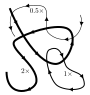
\includegraphics[scale = 0.75]{Multi-structures/Multipaths/multi-path_multiplicity}
}
\end{tabular}

A multi-path \(\mathbf{J}\) is effectively a set of oriented path (\(C\)) / weight (\(w\)) pairs:
\[\mathbf{J} = w_1 C_1 + w_2 C_2 + ... + w_N C_N\]
where \(w_i\) is the weight that is assigned to path \(C_i\). This notation effectively denotes that a multi-path is a collection/sum of oriented paths.

Each weight \(w_i\) will be assumed to be strictly positive, as an oriented path with a weight of 0 is not included as part of the multi-path, and a negative weight can be made positive while reversing the path's orientation. Moreover, the oriented paths will be assumed to all be unique. If a path appears multiple times, then these appearances can be condensed into a single appearance whose weight is the sum of all weights from the multiple appearances. If an oriented path and its reversed orientation appears, then these instances cancel out. The orientation with the smaller weight is eliminated, while the orientation with the larger weight has its weight reduced by the smaller weight. If the weights of both orientations are equal, then the orientations completely cancel each other out. It should also be noted that curves can partially cancel each other out (as illustrated below on the right). 

Two multi-paths are equivalent if and only if the networks of oriented paths are equivalent, regardless of how the network is broken up into individual oriented paths, as illustrated below. In the example on the right, the segments that are on top of each other and have opposite orientations have canceled each other out.    
\begin{center}
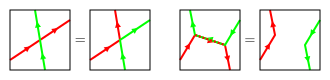
\includegraphics[scale = 0.5]{Multi-structures/Multipaths/multi-path_decomposition}
\end{center}

\begin{center}
\begin{tabular}{cc}
\parbox{0.5\textwidth}{
Unless otherwise specified, no path will be allowed to diverge to points that are infinitely distant.
} & \parbox{0.5\textwidth}{
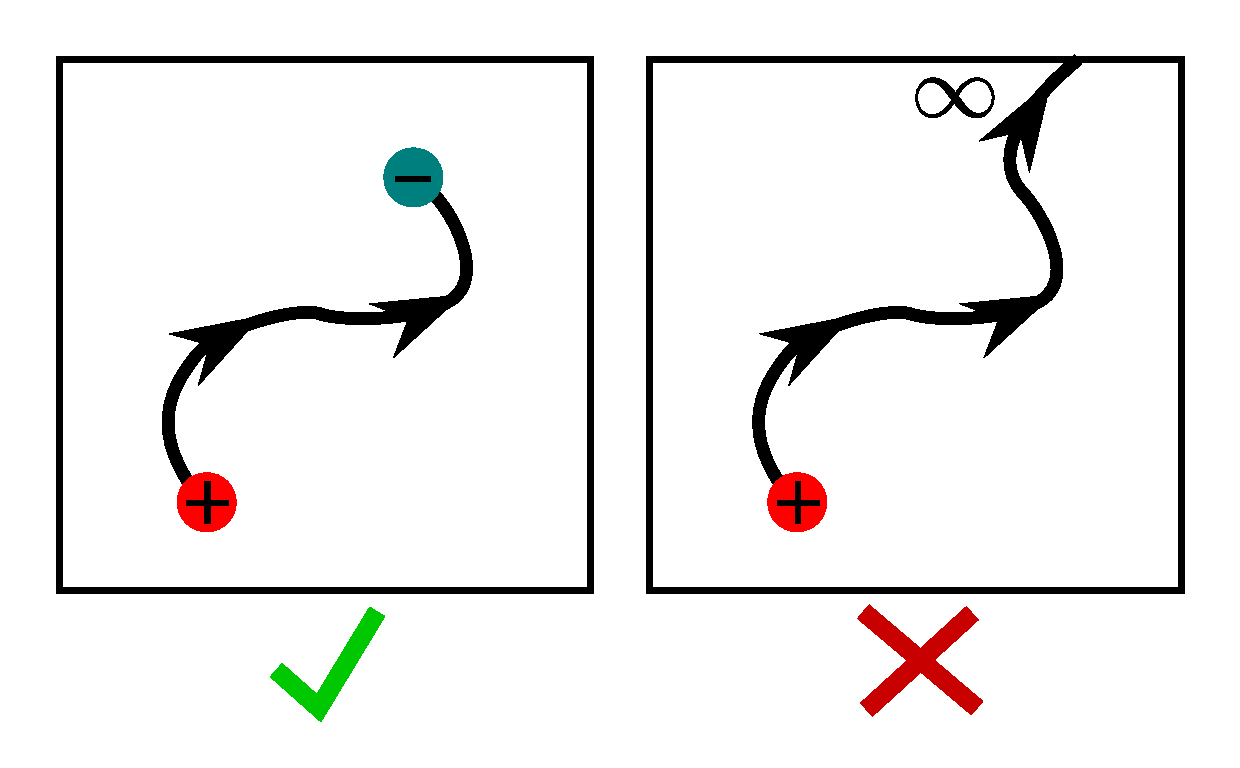
\includegraphics[width = 0.5\textwidth]{Multi-structures/Multipaths/no_infinite_paths}
}
\end{tabular}
\end{center}




\section{Multi-surfaces}

An oriented surface is a surface that has a ``front" side and a ``back" side. The orientation is depicted as arrows that point outwards from the front side, as depicted in the examples below.

\begin{center}
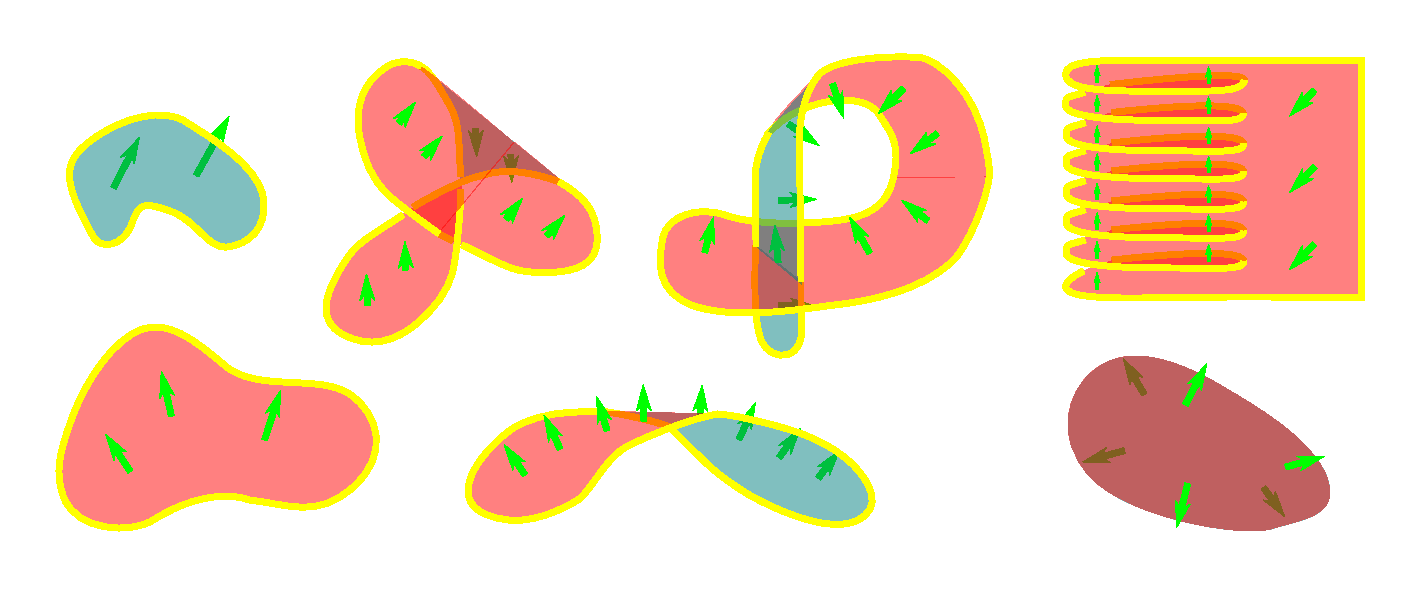
\includegraphics[scale = 0.7]{Multi-structures/Multisurfaces/oriented_surfaces}
\end{center}

A ``Mobius strip" (left) or a ``Klein bottle" (right) are examples of surfaces that have only one side, and therefore cannot be oriented without the introduction of a seam. 

\begin{tabular}{cc}
\parbox{0.5\textwidth}{
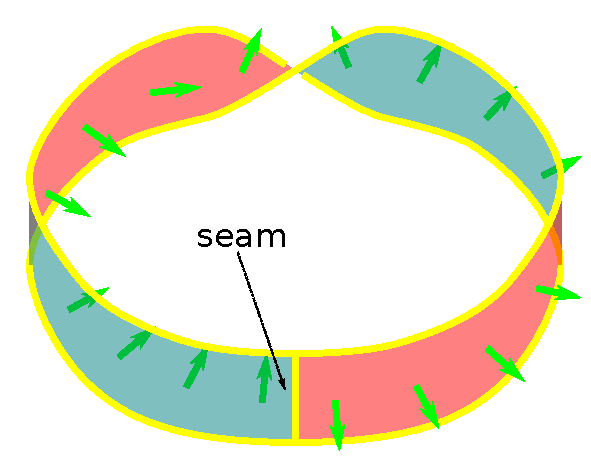
\includegraphics[scale = 0.7]{Multi-structures/Multisurfaces/Mobius_strip}
} & \parbox{0.5\textwidth}{
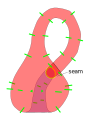
\includegraphics[scale = 0.5]{Multi-structures/Multisurfaces/Klein_bottle}
}
\end{tabular}

\begin{tabular}{cc}
\parbox{0.5\textwidth}{
A \textbf{multi-surface} is a superposition of oriented surfaces. One such superposition is depicted on the right.
} & \parbox{0.5\textwidth}{
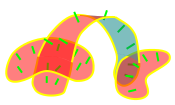
\includegraphics[width = 0.5\textwidth]{Multi-structures/Multisurfaces/multi-surface_simple}
}
\end{tabular}

\begin{tabular}{cc}
\parbox{0.5\textwidth}{
When two oriented surfaces in the same multi-surface are equivalent, the result is the common oriented surface with a weight of \(2\). When three oriented surfaces in the same multi-surface are the equivalent, the result is the common oriented surface with a weight of \(3\). Every oriented surface in a multi-surface has associated with it a ``weight" which is the number of ``stacked" oriented surfaces. The weight can be a fraction, so there can be fractional copies of a surface. {\bf If the weight is negative, then the orientation of the surface is reversed and the sign is flipped to positive.} On the right is a multi-surface where the surfaces have different weights. Note how there are no negative weights, as a negative weight merely flips the orientation of the surface.  
} & \parbox{0.5\textwidth}{
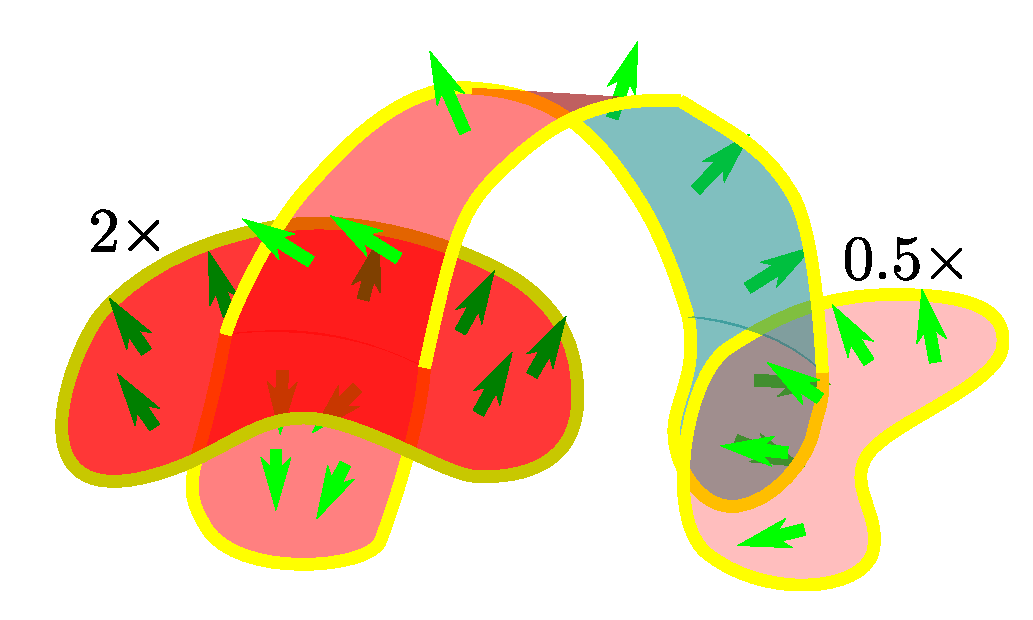
\includegraphics[width = 0.5\textwidth]{Multi-structures/Multisurfaces/multi-surface_multiplicity}
}
\end{tabular}

\vspace{2mm}

A multi-surface \(\mathbf{F}\) is effectively a set of oriented surface (\(\sigma\)) / weight (\(w\)) pairs:
\[\mathbf{F} = w_1 \sigma_1 + w_2 \sigma_2 + ... + w_N \sigma_N\]
where \(w_i\) is the weight that is assigned to surface \(\sigma_i\). This notation effectively denotes that a multi-surface is a collection/sum of oriented surfaces.

As with multi-paths, each weight \(w_i\) will be assumed to be strictly positive, as an oriented surface with a weight of 0 is not included as part of the multi-surface, and a negative weight can be made positive while reversing the surface's orientation. Moreover, the oriented surfaces will be assumed to all be unique. If a surface appears multiple times, then these appearances can be condensed into a single appearance whose weight is the sum of all weights from the multiple appearances. If an oriented surface and its reversed orientation appears, then these instances cancel out. The orientation with the smaller weight is eliminated, while the orientation with the larger weight has its weight reduced by the smaller weight. If the weights of both orientations are equal, then the orientations completely cancel each other out. It should also be noted that surfaces can partially cancel each other out (as illustrated below on the right). 

Two multi-surfaces are equivalent if and only if the networks of oriented surfaces are equivalent, regardless of how the network is broken up into individual oriented surfaces, as illustrated below. In the example on the right, the segments that are on top of each other and have opposite orientations have canceled each other out.     
\begin{center}
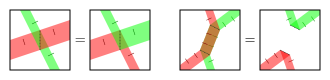
\includegraphics[scale = 0.5]{Multi-structures/Multisurfaces/multi-surface_decomposition}
\end{center}

\begin{center}
\begin{tabular}{cc}
\parbox{0.5\textwidth}{
Unless otherwise specified, no surface will be allowed to diverge to points that are infinitely distant.
} & \parbox{0.5\textwidth}{
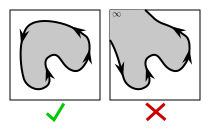
\includegraphics[width = 0.5\textwidth]{Multi-structures/Multisurfaces/no_infinite_surfaces}
}
\end{tabular}
\end{center}





\section{Multi-volumes}

~

\begin{tabular}{cc}
\parbox{0.5\textwidth}{
A \textbf{multi-volume} is a superposition of volumes. One such superposition is depicted on the right.
} & \parbox{0.5\textwidth}{
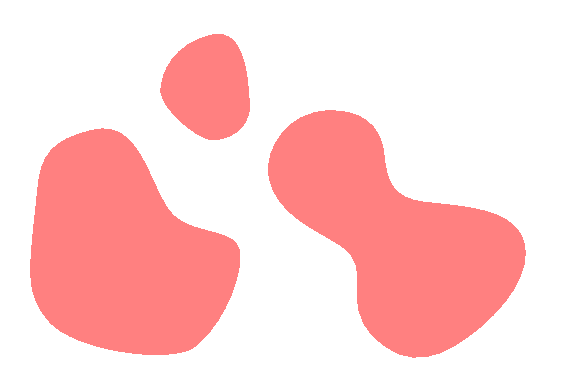
\includegraphics[scale = 0.75]{Multi-structures/Multivolumes/multi-volume_simple}
}
\end{tabular}

\begin{tabular}{cc}
\parbox{0.5\textwidth}{
When two volumes in the same multi-volume are equivalent, the result is the common volume with a weight of \(2\). When three volumes in the same multi-volume are equivalent, the result is the common volume with a weight of \(3\). Every volume in a multi-volume has associated with it a ``weight" which is the number of ``stacked" volumes. The weight can be a fraction, so there can be fractional copies of a volume. The weight can also be negative, so there can be ``anti-volume". If the weight is \(0\), then the volume is simply not included. On the right is a multi-volume, where the volumes have different weights.
} & \parbox{0.5\textwidth}{
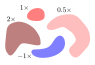
\includegraphics[scale = 0.75]{Multi-structures/Multivolumes/multi-volume_multiplicity}
}
\end{tabular}

\vspace{2mm}

A multi-volume \(U\) is effectively a set of volume (\(\Omega\)) /weight (\(w\)) pairs:
\[U = w_1 \Omega_1 + w_2 \Omega_2 + ... + w_N \Omega_N\]
where \(w_i\) is the weight that is assigned to volume \(\Omega_i\). This notation effectively denotes that a multi-volume is a collection/sum of volumes.

Each weight \(w_i\) will be assumed to be nonzero, as a volume with a weight of 0 is not included as part of the multi-volume. Moreover, the volumes will be assumed to all be unique. If a volume appears multiple times, then these appearances can be condensed into a single appearance whose weight is the sum of all weights from the multiple appearances. It should also be noted that volumes can partially cancel each other out.  

Two multi-volumes \(U_1\) and \(U_2\) are equivalent if and only if at every position \(\mathbf{q}\), the net number of volumes from \(U_1\) that contain \(\mathbf{q}\) is equal to the net number of volumes from \(U_2\) that contain \(\mathbf{q}\). Negative volumes subtract from the number of volumes that contain \(\mathbf{q}\). This is illustrated below. 

Consider the first example on the left. Left of the \(=\) sign, there is a volume with a weight of \(+1\), and a volume with a weight of \(-1\) that overlap. Right of the \(=\) sign, the volume with a weight of \(+1\) has been broken into two separate volumes, and the overlap has been canceled out. {\bf These two multi-volumes are equivalent.} 

Consider the second example on the right. Left of the \(=\) sign, there is a volume with a weight of \(+1\), and a volume with a weight of \(-1\) that overlap each other. Right of the \(=\) sign, the intersection has been canceled out, breaking each of the volumes into 2 separate pieces. {\bf These two multi-volumes are equivalent.}  

\begin{center}
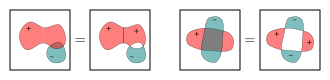
\includegraphics[scale = 0.5]{Multi-structures/Multivolumes/multi-volume_decomposition}
\end{center}

In general, given an arbitrary position \(\mathbf{q}\), and a multi-volume \(U\), the notation \(U(\mathbf{q})\) will denote the net number of volumes that contain \(\mathbf{q}\). Multi-volumes \(U_1\) and \(U_2\) are equivalent if and only if \(U_1(\mathbf{q}) = U_2(\mathbf{q})\) at all positions \(\mathbf{q}\). 

\begin{center}
\begin{tabular}{cc}
\parbox{0.5\textwidth}{
Unless otherwise specified, no volume will be allowed to diverge to points that are infinitely distant.
} & \parbox{0.5\textwidth}{
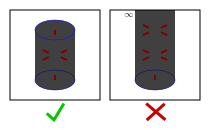
\includegraphics[width = 0.5\textwidth]{Multi-structures/Multivolumes/no_infinite_volumes}
}
\end{tabular}
\end{center}



\section{Summary}

This chapter gave an introduction to the 4 types of multi-structures that will be used in the beginning chapters of this book: multi-points; multi-paths; multi-surfaces; and multi-volumes. In the later chapters when time is introduced as a factor, an additional multi-structure called ``multi-events" will be introduced.





\chapter{Unions}

\section{Introduction}

This chapter will consist of a brief discussion of how multi-structures are ``summed". The sum is similar to computing the union of sets (more specifically multi-sets), but with major differences as will soon become apparent.

A ``union" between two multi-structures of the same ``type" is the result of simply ``combining" the multi-structures in a straightforwards manner. The addition symbol ``\(+\)" denotes the union. The union of two sets typically counts the elements that are common to both sets only once, but here {\bf the weights of structures that are common to both multi-structures are added together}. 

{\bf Only multi-structures with the same type can be summed. The sum/union of multi-structures of different types will not be considered.} 


\section{point-point unions}

\vspace{5mm}

\begin{tabular}{cc}
\parbox{0.5\textwidth}{
The union of multi-points \(\rho_1\) and \(\rho_2\) is the set of all weighted points from both multi-points. If the same points appear then their weights are added. If any resultant weight is \(0\), then the corresponding point disappears.  

An example of such a multi-point union is depicted on the right. Illustrated are examples of points stacking up to form points of greater weight, and points canceling out, partially as well as completely. 
} & \parbox{0.5\textwidth}{
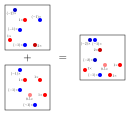
\includegraphics[width = 0.5\textwidth]{Unions/multipoint_unions}
}
\end{tabular}

Lastly, given a multi-point \(\rho\) and a positive integer \(n\), then
\[n \cdot \rho = \underbrace{\rho + \rho + ... + \rho}_n\]
so ``multiplying" a multi-point by \(n\) is to multiply the weight of each point by \(n\). More generally, to multiply a multi-point by any real number \(k\) is to multiply the weight of each point by \(k\). ``Multiplication" by \(k\) is denoted by:
\[k \cdot \rho \quad\quad\text{or}\quad\quad k\rho \quad\quad\text{or}\quad\quad \rho \cdot k \quad\quad\text{or}\quad\quad \rho k\]


\section{path-path unions}

\vspace{5mm}

\begin{tabular}{cc}
\parbox{0.5\textwidth}{
The union of multi-paths \(\mathbf{J}_1\) and \(\mathbf{J}_2\) is the set of all weighted oriented paths from both multi-paths. An example of such a union is depicted on the right. Illustrated are examples of paths with identical orientation stacking to form paths with a greater weight, and paths with opposite orientation canceling out.
} & \parbox{0.5\textwidth}{
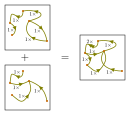
\includegraphics[width = 0.5\textwidth]{Unions/multipath_unions}
}
\end{tabular}

Lastly, given a multi-path \(\mathbf{J}\) and a positive integer \(n\), then
\[n \cdot \mathbf{J} = \underbrace{\mathbf{J} + \mathbf{J} + ... + \mathbf{J}}_n\]
so ``multiplying" a multi-path by \(n\) is to multiply the weight of each path by \(n\). More generally, to multiply a multi-path by any real number \(k\) is to multiply the weight of each path by \(k\), reversing the orientation of paths with negative weight. ``Multiplication" by \(k\) is denoted by:
\[k \cdot \mathbf{J} \quad\quad\text{or}\quad\quad k\mathbf{J} \quad\quad\text{or}\quad\quad \mathbf{J} \cdot k \quad\quad\text{or}\quad\quad \mathbf{J} k\]


\section{surface-surface unions}

\vspace{5mm}

\begin{tabular}{cc}
\parbox{0.5\textwidth}{
The union of multi-surfaces \(\mathbf{F}_1\) and \(\mathbf{F}_2\) is the set of all weighted oriented surfaces from both multi-surfaces. An example of such a union is depicted on the right (using 2D cross-sections). Illustrated are examples of surfaces with identical orientation stacking to form surfaces with a greater weight, and surfaces with opposite orientation canceling out, partially as well as completely.
} & \parbox{0.5\textwidth}{
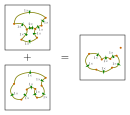
\includegraphics[width = 0.5\textwidth]{Unions/multisurface_unions}
}
\end{tabular}

Lastly, given a multi-surface \(\mathbf{F}\) and a positive integer \(n\), then
\[n \cdot \mathbf{F} = \underbrace{\mathbf{F} + \mathbf{F} + ... + \mathbf{F}}_n\]
so ``multiplying" a multi-surface by \(n\) is to multiply the weight of each surface by \(n\). More generally, to multiply a multi-surface by any real number \(k\) is to multiply the weight of each surface by \(k\), reversing the orientation of surfaces with negative weight. ``Multiplication" by \(k\) is denoted by:
\[k \cdot \mathbf{F} \quad\quad\text{or}\quad\quad k\mathbf{F} \quad\quad\text{or}\quad\quad \mathbf{F} \cdot k \quad\quad\text{or}\quad\quad \mathbf{F} k\]



\section{volume-volume unions}

\vspace{5mm}

\begin{tabular}{cc}
\parbox{0.5\textwidth}{
The union of multi-volumes \(U_1\) and \(U_2\) is the set of all weighted volumes from both multi-volumes. An example of such a union is depicted on the right (using 2D cross-sections). Illustrated are examples of volumes partially canceling each other out. Note that for a specific point \(\mathbf{q}\), that the net number of volumes that contain \(\mathbf{q}\) in the union \(U_1 + U_2\) will always be the sum of the net number of volumes that contain \(\mathbf{q}\) in each of \(U_1\) and \(U_2\): 
\[(U_1 + U_2)(\mathbf{q}) = U_1(\mathbf{q}) + U_2(\mathbf{q})\]
} & \parbox{0.5\textwidth}{
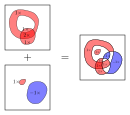
\includegraphics[width = 0.5\textwidth]{Unions/multivolume_unions}
}
\end{tabular}

Lastly, given a multi-volume \(U\) and a positive integer \(n\), then
\[n \cdot U = \underbrace{U + U + ... + U}_n\]
so ``multiplying" a multi-volume by \(n\) is to multiply the weight of each volume by \(n\). More generally, to multiply a multi-volume by any real number \(k\) is to multiply the weight of each volume by \(k\). ``Multiplication" by \(k\) is denoted by:
\[k \cdot U \quad\quad\text{or}\quad\quad k U \quad\quad\text{or}\quad\quad U \cdot k \quad\quad\text{or}\quad\quad U k\]




\section{Summary}

This chapter was a brief formalization of the union of two multi-structures with the same type. The union of multi-structures with different types is not allowed.





\chapter{Intersections}

\section{Introduction}

The previous chapter discussed the union between two multi-structures, this chapter will discuss the intersection between two multi-structures. The important difference is that while the union required that both multi-structures have the same type, intersections can occur between structures with different types. In fact for some of the low dimensionality multi-structures such as points and paths, the intersection of two of these structure will not even be considered.

As is expected, the intersection of two structures is often the set of positions that are common to both structures, but this will not always be the case. 6 types of intersections will be considered: 
\begin{itemize}
\item point-volume intersections 
\item path-surface intersections 
\item path-volume intersections 
\item surface-surface intersections 
\item surface-volume intersections 
\item volume-volume intersections
\end{itemize}
Other intersections will not be considered, for reasons primarily related to the fact that such intersections cannot be oriented, as will be discussed later. Intersections are generally denoted with the symbol \(\cap\), but more specialized symbols will be introduced for each of the specific 6 types of intersections that are begin considered. 

\vspace{5mm}

\begin{tabular}{cc}
\parbox{0.5\textwidth}{
One property of intersections that will be used heavily is {\bf linearity}. Given a set \(A\) and two sets \(B\) and \(C\), the intersection of \(A\) with the union \(B + C\) is the sum of the intersection of \(A\) with \(B\) separately and the intersection with \(A\) with \(C\) separately. This property is referred to as ``linearity", and is also frequently referred to as the ``distributive law":

\[A \cap (B + C) = (A \cap B) + (A \cap C)\]

\[(B + C) \cap A = (B \cap A) + (C \cap A)\]

More generally if \(k\) is a real number, then the intersection of \(A\) with \(k\) copies of \(B\) is \(k\) copies of the intersection of \(A\) with \(B\):

\[A \cap (k \cdot B) = k(A \cap B)\]

\[(k \cdot A) \cap B = k(A \cap B)\]

} & \parbox{0.5\textwidth}{
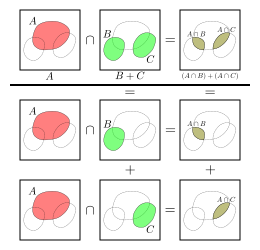
\includegraphics[width = 0.5\textwidth]{Intersections/intersection_distributive_law}
}
\end{tabular}





\section{Point-volume intersections}

Given a multi-point \(\rho\) and a multi-volume \(U\), then the intersection between \(\rho\) and \(U\) is a multi-point and is denoted by:

\[\rho \cdot U \quad\quad\text{or}\quad\quad \rho U \quad\quad\text{or}\quad\quad U \cdot \rho \quad\quad\text{or}\quad\quad U \rho\]

Given a single point \(P\), and a single volume \(\Omega\), the intersection is \(P\) if \(P\) is contained by \(\Omega\), and is nothing if \(P\) is not contained by \(\Omega\). 

If a point \(P\) with a weight of \(w_1\) is contained in a volume \(\Omega\) with a weight of \(w_2\), then for each of the \(w_2\) copies of \(\Omega\), \(w_1\) copies of \(P\) are intersecting that copy. The total intersection is \(w_1 \cdot w_2\) copies of \(P\):
\[(w_1 P) \cdot (w_2\Omega) = w_1w_2P\]      

If a point \(P\) with a weight of \(w_1\) is {\bf not} contained in a volume \(\Omega\) with a weight of \(w_2\), then for each of the \(w_2\) copies of \(\Omega\), \(w_1\) copies of \(P\) are not intersecting that copy. The total intersection is nothing:
\[(w_1 P) \cdot (w_2\Omega) = 0\]      

Given a multi-point \(\rho = w_1 P_1 + w_2 P_2 + ... + w_N P_N\) and a multi-volume \\ \(U = v_1\Omega_1 + v_2\Omega_2 + v_M\Omega_M\), then the intersection \(\rho \cdot U\) is the set of all pairwise intersections of the points and volumes:
\begin{align*}
\rho \cdot U = & \left\{\begin{array}{c}
\;\; w_1 v_1 (P_1 \cdot \Omega_1) + w_1 v_2 (P_1 \cdot \Omega_2) + \cdots + w_1 v_M (P_1 \cdot \Omega_M) \\ 
+ w_2 v_1 (P_2 \cdot \Omega_1) + w_2 v_2 (P_2 \cdot \Omega_2) + \cdots + w_2 v_M (P_2 \cdot \Omega_M) \\ 
\vdots \\
+ w_N v_1 (P_N \cdot \Omega_1) + w_N v_2 (P_N \cdot \Omega_2) + \cdots + w_N v_M (P_N \cdot \Omega_M) \\ 
\end{array}\right.
\end{align*}

In general,
\begin{itemize}
\item Given multi-points \(\rho_1\) and \(\rho_2\), and multi-volume \(U\), then:
\[(\rho_1 + \rho_2) \cdot U = \rho_1 \cdot U + \rho_2 \cdot U\] 
\item Given multi-point \(\rho\), multi-volume \(U\), and some real number \(c\), then:
\[(c\rho) \cdot U = c(\rho \cdot U)\]
\item Given multi-point \(\rho\), and multi-volumes \(U_1\) and \(U_2\), then:
\[\rho \cdot (U_1 + U_2) = \rho \cdot U_1 + \rho \cdot U_2\] 
\item Given multi-point \(\rho\), multi-volume \(U\), and some real number \(c\), then:
\[\rho \cdot (cU) = c(\rho \cdot U)\]
\end{itemize}

%Some examples of this {\bf distributive law} are listed below:
%\begin{itemize}
%\item Assume that \(P\) is contained by \(\Omega\). Given \(2\) copies of point \(P\), the intersection of the multi-point \(2P\) with the multi-volume \(\Omega\) is again 2 copies of \(P\): \((2P) \cdot \Omega = 2P\). Given an anti-copy of point \(P\), the intersection of the multi-point \(-P\) with the multi-volume \(\Omega\) is an anti-copy of \(P\): \((-P) \cdot \Omega = -P\).
%\item Assume that \(P\) is contained by \(\Omega\). Given \(2\) copies of volume \(\Omega\), the intersection of the multi-point \(P\) with the multi-volume \(2\Omega\) is again 2 copies of \(P\), since \(P\) is contained by \(2\) volumes: \(2P\). Given an anti-copy of volume \(\Omega\), the intersection of the multi-point \(P\) with the multi-volume \(-\Omega\) is an anti-copy of \(P\), since \(P\) is contained in an anti-volume: \(-P\).    
%\end{itemize}

\begin{center}
\begin{tabular}{cc}
\parbox{0.5\textwidth}{
An example of how the intersection of a multi-point and a multi-volume is the set of all pairwise intersections between the points and volumes will be given. On the right, the fact that the intersection consists of all pairs of intersections between points and volumes is illustrated with a simple example. There are two points \(P_1\) and \(P_2\), and two volumes \(\Omega_1\) and \(\Omega_2\). Points \(P_1\) and \(P_2\) are both contained in \(\Omega_1\) and \(\Omega_2\). Consider the multi-point \(\rho = P_1 + P_2\), and the multi-volume \(U = \Omega_1 + \Omega_2\). 

\(P_1\) is contained in \(\Omega_1\) so \(P_1 \cdot \Omega_1 = P_1\).  

\(P_1\) is contained in \(\Omega_2\) so \(P_1 \cdot \Omega_2 = P_1\).

\(P_2\) is contained in \(\Omega_1\) so \(P_2 \cdot \Omega_1 = P_2\).

\(P_2\) is contained in \(\Omega_2\) so \(P_2 \cdot \Omega_2 = P_2\).

The total intersection of \(\rho\) with \(U\) consists of all of the pairwise intersections:

\begin{align*}
\rho \cdot U & = P_1 + P_1 + P_2 + P_2 
= 2P_1 + 2P_2  
\end{align*}
} & \parbox{0.5\textwidth}{
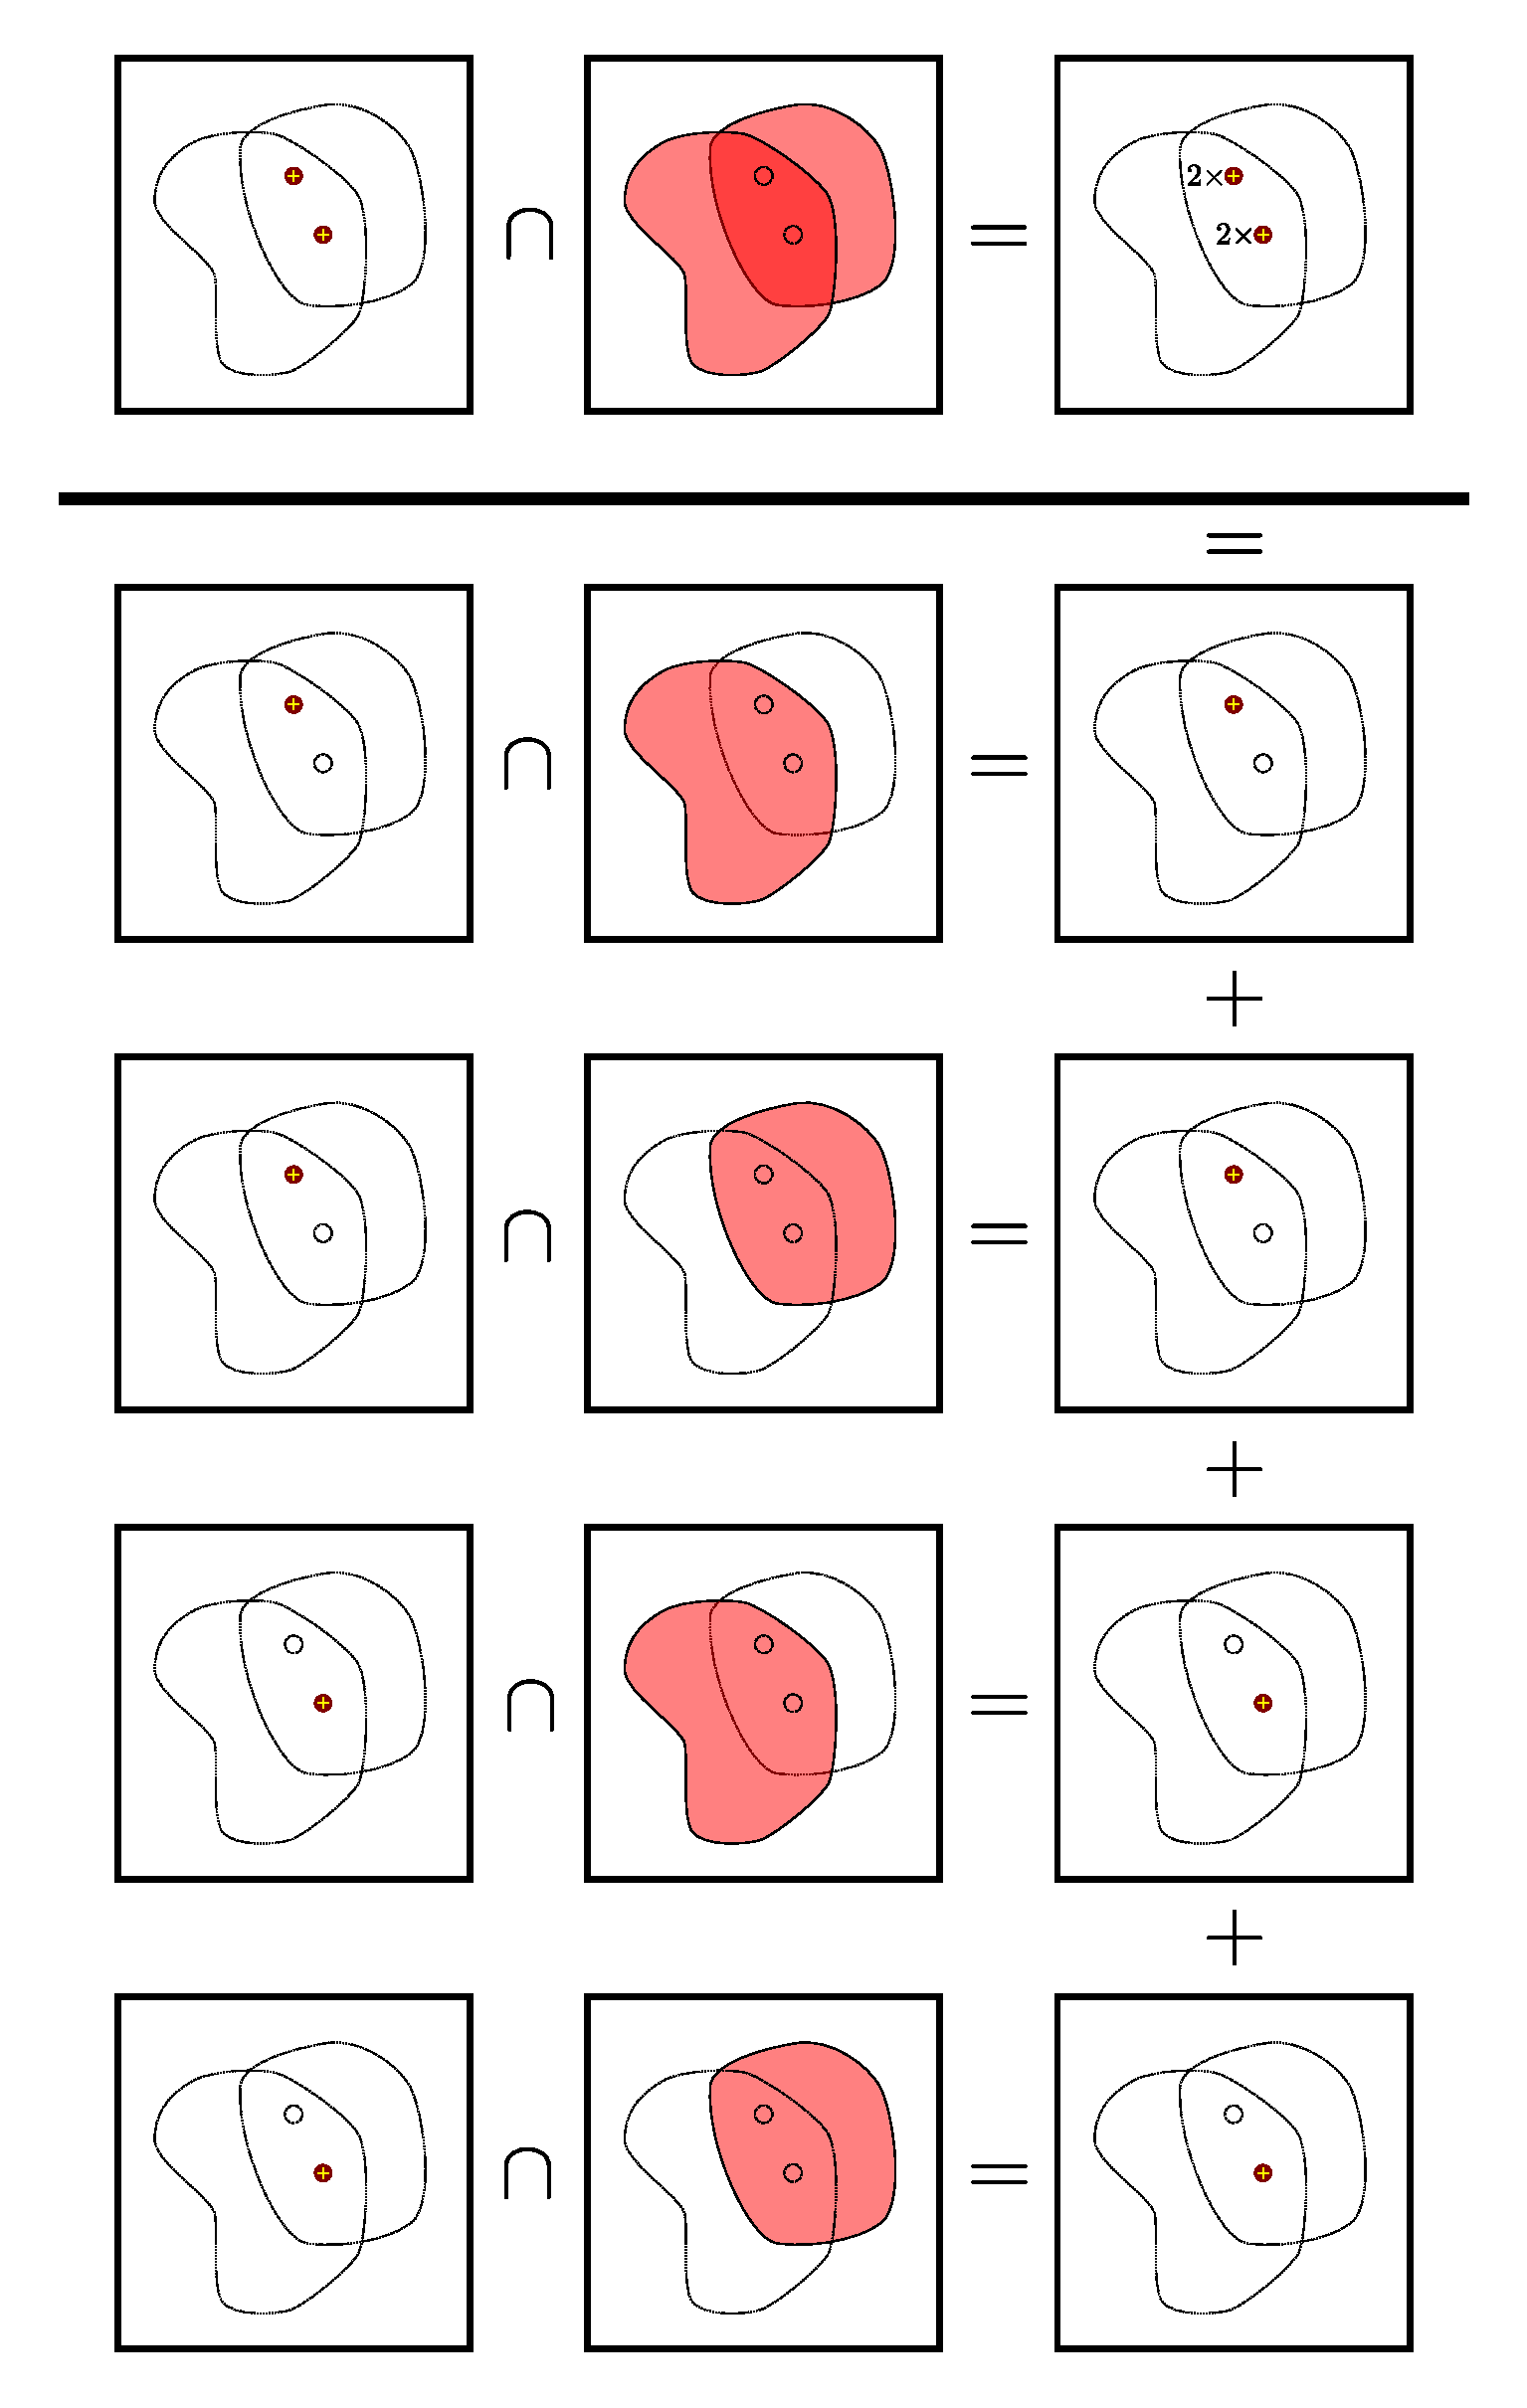
\includegraphics[width = 0.5\textwidth]{Intersections/Point-volume_intersections/point_volume_intersection_distributive_law}
}
\end{tabular}
\end{center} 

In the example below, the intersection between a multi-point and a multi-volume is illustrated. Note how the points that fall inside the negative volume have their polarities reversed. 

\begin{center}
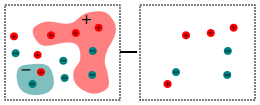
\includegraphics[scale = 0.4]{Intersections/Point-volume_intersections/point_volume_intersections_two_panel_example}
\end{center}

\begin{tabular}{cc}
\parbox{0.5\textwidth}{
If a point \(P\) with a weight of \(1\) lies on the edge of a volume with a weight of \(1\), then the intersection point \(P\) has a weight of \(0.5\).
} & \parbox{0.5\textwidth}{
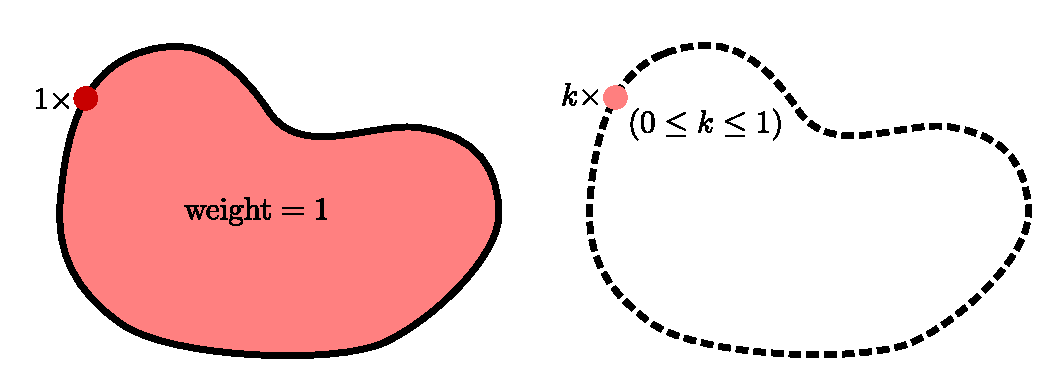
\includegraphics[width = 0.5\textwidth]{Intersections/Point-volume_intersections/point_volume_intersection_boundary_case}
}
\end{tabular}





\section{Path-surface intersections}

Given a multi-path \(\mathbf{J}\) and a multi-surface \(\mathbf{F}\), then the intersection between \(\mathbf{J}\) and \(\mathbf{F}\) is a multi-point and is denoted by:

\[\mathbf{J} \bullet \mathbf{F} \quad\quad\text{or}\quad\quad \mathbf{F} \bullet \mathbf{J}\]

An intersection occurs when a path pierces a surface. If a path with a weight of \(1\) pierces a surface with a weight of \(1\) in the preferred direction, then the intersection point has a weight of \(+1\). If a path with a weight of \(1\) pierces a surface with a weight of \(1\) in the opposite direction, then the intersection point has a weight of \(-1\). The ``preferred direction" is when the path enters the surface from the back and emerges from the front. The opposite direction is when the path enters the surface from the front and emerges from the back.

In the examples below, the intersection points have a positive weight when the path intersects the surface in the preferred direction, and the intersection points have a negative weight when the path intersects the surface in the reverse direction.

\begin{tabular}{cc}
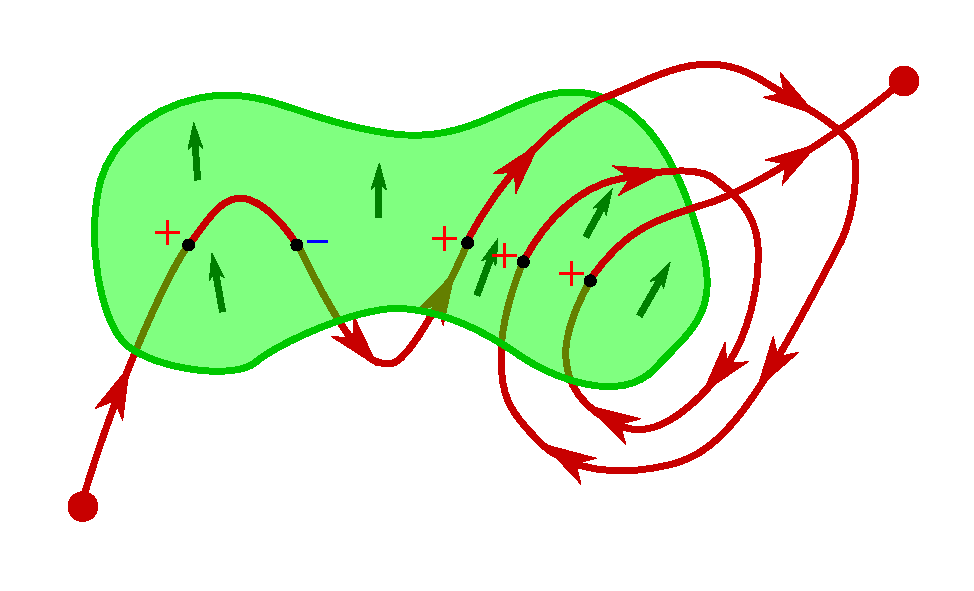
\includegraphics[width = 0.5\textwidth]{Intersections/Path-surface_intersections/path_surface_intersections}
& 
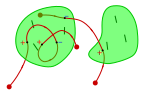
\includegraphics[width = 0.5\textwidth]{Intersections/Path-surface_intersections/path_surface_intersections_2}
\end{tabular}

If a path \(C\) with a nonnegative weight of \(w_1\) intersects a surface \(\sigma\) with a nonnegative weight of \(w_2\) in the {\bf preferred direction} at point \(P\), then for each of the \(w_2\) copies of \(\sigma\), \(w_1\) copies of \(C\) are intersecting that copy. The total intersection is \(w_1 \cdot w_2\) copies of \(P\):
\[(w_1 C) \bullet (w_2\sigma) = w_1 w_2 P\] 

Contrariwise, if a path \(C\) with a weight of \(w_1\) intersects a surface \(\sigma\) with a weight of \(w_2\) in the {\bf opposite direction} at point \(P\), then for each of the \(w_2\) copies of \(\sigma\), \(w_1\) copies of \(C\) are intersecting that copy in the opposite direction. The total intersection is \(w_1 \cdot w_2\) copies of the anti-point \(-P\):
\[(w_1 C) \bullet (w_2 \sigma) = -w_1 w_2 P\]  

Given a multi-path \(\mathbf{J} = w_1C_1 + w_2C_2 + ... + w_NC_N\) and a multi-surface \\ \(\mathbf{F} = v_1\sigma_1 + v_2\sigma_2 + ... + v_M\sigma_M\), then the intersection \(\mathbf{J} \bullet \mathbf{F}\) is the set of all pairwise intersections of the paths and surfaces:
\begin{align*}
\mathbf{J} \bullet \mathbf{F} = & \left\{\begin{array}{c}
\;\; w_1 v_1 (C_1 \bullet \sigma_1) + w_1 v_2 (C_1 \bullet \sigma_2) + \cdots + w_1 v_M (C_1 \bullet \sigma_M) \\ 
+ w_2 v_1 (C_2 \bullet \sigma_1) + w_2 v_2 (C_2 \bullet \sigma_2) + \cdots + w_2 v_M (C_2 \bullet \sigma_M) \\ 
\vdots \\
+ w_N v_1 (C_N \bullet \sigma_1) + w_N v_2 (C_N \bullet \sigma_2) + \cdots + w_N v_M (C_N \bullet \sigma_M) \\ 
\end{array}\right.
\end{align*}

In general,
\begin{itemize}
\item Given multi-paths \(\mathbf{J}_1\) and \(\mathbf{J}_2\), and multi-surface \(\mathbf{F}\), then:
\[(\mathbf{J}_1 + \mathbf{J}_2) \bullet \mathbf{F} = \mathbf{J}_1 \bullet \mathbf{F} + \mathbf{J}_2 \bullet \mathbf{F}\] 
\item Given multi-path \(\mathbf{J}\), multi-surface \(\mathbf{F}\), and some real number \(c\), then:
\[(c\mathbf{J}) \bullet \mathbf{F} = c(\mathbf{J} \bullet \mathbf{F})\]
\item Given multi-path \(\mathbf{J}\), and multi-surfaces \(\mathbf{F}_1\) and \(\mathbf{F}_2\), then:
\[\mathbf{J} \bullet (\mathbf{F}_1 + \mathbf{F}_2) = \mathbf{J} \bullet \mathbf{F}_1 + \mathbf{J} \bullet \mathbf{F}_2\] 
\item Given multi-path \(\mathbf{J}\), multi-surface \(\mathbf{F}\), and some real number \(c\), then:
\[\mathbf{J} \bullet (c\mathbf{F}) = c(\mathbf{J} \bullet \mathbf{F})\]
\end{itemize}

\begin{center}
\begin{tabular}{cc}
\parbox{0.5\textwidth}{
An example of how the intersection of a multi-path and a multi-surface is the set of all pairwise intersections between the paths and surfaces will be given. On the right, the fact that the intersection consists of all pairs of intersections between paths and surfaces is illustrated with a simple example. There are two oriented paths \(C_1\) and \(C_2\), and two oriented surfaces \(\sigma_1\) and \(\sigma_2\). Paths \(C_1\) and \(C_2\) both pass through \(\sigma_1\) and \(\sigma_2\) in the preferred direction. Consider the multi-path \(\mathbf{J} = C_1 + C_2\), and the multi-surface \(\mathbf{F} = \sigma_1 + \sigma_2\). 

The intersection of \(C_1\) with \(\sigma_1\) is a point \(P_{1,1}\) so \\ \(C_1 \bullet \sigma_1 = P_{1,1}\)  

The intersection of \(C_1\) with \(\sigma_2\) is a point \(P_{1,2}\) so \\ \(C_1 \bullet \sigma_2 = P_{1,2}\)  

The intersection of \(C_2\) with \(\sigma_1\) is a point \(P_{2,1}\) so \\ \(C_2 \bullet \sigma_1 = P_{2,1}\)  

The intersection of \(C_2\) with \(\sigma_2\) is a point \(P_{2,2}\) so \\ \(C_2 \bullet \sigma_2 = P_{2,2}\)  

The total intersection of \(\mathbf{J}\) with \(\mathbf{F}\) consists of all of the pairwise intersections:

\begin{align*}
\mathbf{J} \bullet \mathbf{F} & = P_{1,1} + P_{1,2} + P_{2,1} + P_{2,2} 
\end{align*}
} & \parbox{0.4\textwidth}{
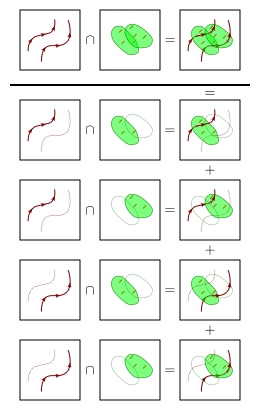
\includegraphics[width = 0.4\textwidth]{Intersections/Path-surface_intersections/path_surface_intersection_distributive_law}
}
\end{tabular}
\end{center}

If a path \(C\) fails to fully pass through a surface \(\sigma\), then the weight of the intersection point is halved. {\bf Paths that are embedded inside of surfaces do contribute any intersection points unless they enter or leave the surface.} It may be argued that all points along an embedded path should be counted as intersection points, but the counter argument is to ask what polarity these points should have.

If path \(C\) enters the back of \(\sigma\) and then continues inside of \(\sigma\), then the point where \(C\) first touches \(\sigma\) has a weight of \(+0.5\). If path \(C\) enters the front of \(\sigma\) and then continues inside of \(\sigma\), then the point where \(C\) first touches \(\sigma\) has a weight of \(-0.5\). 

If \(C\) is inside of \(\sigma\) and then exits the front of \(\sigma\), then the exit point has a weight of \(+0.5\). If \(C\) is inside of \(\sigma\) and then exits the back of \(\sigma\), then the exit point has a weight of \(-0.5\). 

\begin{center}
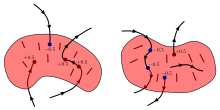
\includegraphics[width = 0.75\textwidth]{Intersections/Path-surface_intersections/path_surface_intersection_boundary_case}
\end{center}

Moreover, if the path \(C\) clips the boundary of \(\sigma\), then the weight of the intersection point is also halved.





\section{Path-volume intersections}

Given a multi-path \(\mathbf{J}\) and a multi-volume \(U\), then the intersection between \(\mathbf{J}\) and \(U\) is a multi-path and is denoted by:

\[\mathbf{J} \cdot U \quad\quad\text{or}\quad\quad \mathbf{J} U \quad\quad\text{or}\quad\quad U \cdot \mathbf{J} \quad\quad\text{or}\quad\quad U \mathbf{J}\]

Given an oriented path \(C\), and a volume \(\Omega\), then the intersection is the sections of \(C\) that are contained in \(\Omega\). If the weight of \(\Omega\) is negative, then the orientation of the intersection is reversed. % The intersection is the sections of \(\mathbf{J}\) that are embedded in \(\mathbf{U}\). If the volume 

In the examples below, only sections of the path that are contained inside a volume are part of the intersection.

\begin{center}
\begin{tabular}{cc}
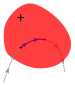
\includegraphics[width = 0.3\textwidth]{Intersections/Path-volume_intersections/path_volume_intersections_example}
& 
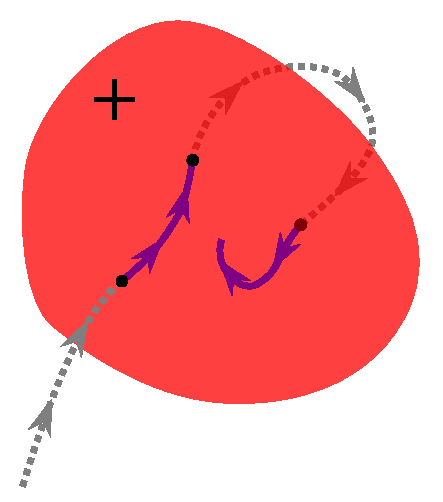
\includegraphics[width = 0.3\textwidth]{Intersections/Path-volume_intersections/path_volume_intersections_example_2}
\end{tabular}
\end{center}

If a path \(C\) with a nonnegative weight of \(w_1\) intersects a volume \(\Omega\) with a weight of \(w_2\), and \(C'\) is the sections of \(C\) that are contained in \(\Omega\), then for each of the \(w_2\) copies of \(\Omega\), \(w_1\) copies of \(C\) are intersecting that copy. The total intersection is \(w_1 \cdot w_2\) copies of \(C'\):
\[(w_1 C) \cdot (w_2 \Omega) = w_1 w_2 C'\] 
If the volume weight \(w_2\) is negative, then both the orientation of \(C'\) and the sign of the weight \(w_1 w_2\) is flipped. 

Given a multi-path \(\mathbf{J} = w_1 C_1 + w_2 C_2 + ... + w_N C_N\) and a multi-volume \\ \(U = v_1 \Omega_1 + v_2\Omega_2 + ... + v_M\Omega_M\), then the intersection \(\mathbf{J} \cdot U\) is the set of all pairwise intersections of the paths and volumes:
\begin{align*}
\mathbf{J} \cdot U = & \left\{\begin{array}{c}
\;\; w_1 v_1 (C_1 \cdot \Omega_1) + w_1 v_2 (C_1 \cdot \Omega_2) + \cdots + w_1 v_M (C_1 \cdot \Omega_M) \\ 
+ w_2 v_1 (C_2 \cdot \Omega_1) + w_2 v_2 (C_2 \cdot \Omega_2) + \cdots + w_2 v_M (C_2 \cdot \Omega_M) \\ 
\vdots \\
+ w_N v_1 (C_N \cdot \Omega_1) + w_N v_2 (C_N \cdot \Omega_2) + \cdots + w_N v_M (C_N \cdot \Omega_M) \\ 
\end{array}\right.
\end{align*}

In general,
\begin{itemize}
\item Given multi-paths \(\mathbf{J}_1\) and \(\mathbf{J}_2\), and multi-volume \(U\), then:
\[(\mathbf{J}_1 + \mathbf{J}_2) \cdot U = \mathbf{J}_1 \cdot U + \mathbf{J}_2 \cdot U\] 
\item Given multi-path \(\mathbf{J}\), multi-volume \(U\), and some real number \(c\), then:
\[(c\mathbf{J}) \cdot U = c(\mathbf{J} \cdot U)\]
\item Given multi-path \(\mathbf{J}\), and multi-volumes \(U_1\) and \(U_2\), then:
\[\mathbf{J} \cdot (U_1 + U_2) = \mathbf{J} \cdot U_1 + \mathbf{J} \cdot U_2\] 
\item Given multi-path \(\mathbf{J}\), multi-volume \(U\), and some real number \(c\), then:
\[\mathbf{J} \cdot (cU) = c(\mathbf{J} \cdot U)\]
\end{itemize}

In the example below, the multi-volume \(U\) consists of three volumes. Two of the volumes have a weight of \(+1\) and are overlapping, and the remaining separate volume has a weight of \(-1\). The multi-path \(\mathbf{J}\) consists of a single path that winds through each of the volumes. Outside of all of the volumes, the path is not part of the intersection. Where the path is passing through a single volume with a weight of \(+1\), the intersection path from \(\mathbf{J} \cdot U\) has a weight of \(+1\). Where the path is passing through the overlap between the volumes with a weight of \(+1\), then each volume contributes a copy of the intersection to \(\mathbf{J} \cdot U\) so the weight of the path in \(\mathbf{J} \cdot U\) is \(+2\). Where the path is passing through the volume with a weight of \(-1\), the orientation of the intersection is reversed.  

\begin{center}
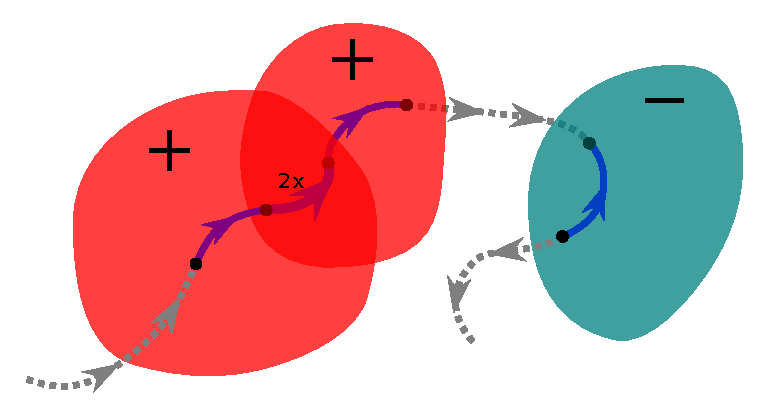
\includegraphics[width = 0.75\textwidth]{Intersections/Path-volume_intersections/path_volume_intersections_example_3}
\end{center}


\begin{tabular}{cc}
\parbox{0.5\textwidth}{
If a path \(C\) is on the surface of volume \(\Omega\), then the intersection is \(C\) with a weight of \(+0.5\) as depicted on the right.
} & \parbox{0.5\textwidth}{
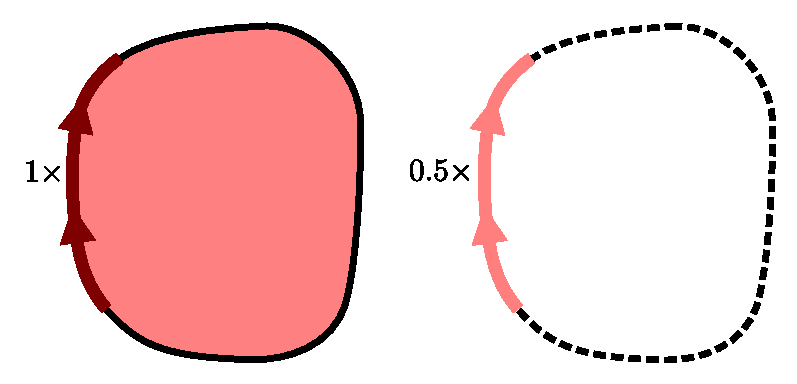
\includegraphics[width = 0.5\textwidth]{Intersections/Path-volume_intersections/path_volume_intersection_boundary_case}
}
\end{tabular}






\section{Surface-surface intersections}

Given two multi-surfaces \(\mathbf{F}_1\) and \(\mathbf{F}_2\), then the intersection between \(\mathbf{F}_1\) and \(\mathbf{F}_2\) is a multi-path and is denoted by:

\[\mathbf{F}_1 \times \mathbf{F}_2\]

An intersection occurs when a surface slices into another surface along a curve. The orientation of the intersection curve is now to be determined. 

\begin{tabular}{cc}
\parbox{0.5\textwidth}{
Given two oriented surfaces \(\sigma_1\) and \(\sigma_2\), the orientation of the intersection \(C\) can be determined as follows. Position your view point in the space that contains the front of \(\sigma_1\) and \(\sigma_2\). When the \(\sigma_1\) is on your left, and \(\sigma_2\) is on your right, then the intersection is oriented towards you as depicted on the right. This is commonly referred to as the ``righthand rule".
} & \parbox{0.5\textwidth}{
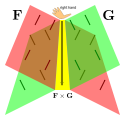
\includegraphics[width = 0.5\textwidth]{Intersections/Surface-surface_intersections/right_hand_rule}
}
\end{tabular}

Some examples are shown below:

\begin{center}
\begin{tabular}{cc}
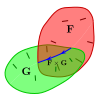
\includegraphics[width = 0.4\textwidth]{Intersections/Surface-surface_intersections/surface_surface_intersections_example}
& 
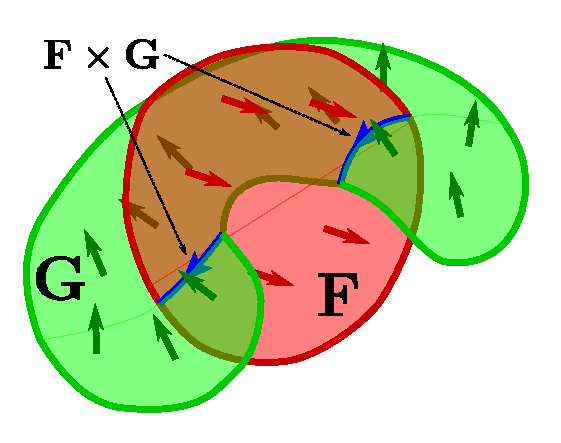
\includegraphics[width = 0.4\textwidth]{Intersections/Surface-surface_intersections/surface_surface_intersections_example_2}
\end{tabular}
\end{center}

Unlike other intersections, the ``order" of the two surfaces impacts the orientation of the intersection path. If the order of the surfaces is reversed, then the orientation of the intersection path is also reversed:

\[\sigma_2 \cap \sigma_1 = -(\sigma_1 \cap \sigma_2)\]

so:

\begin{thm}
\[\mathbf{F}_2 \times \mathbf{F}_1 = -(\mathbf{F}_1 \times \mathbf{F}_2)\]
\end{thm}

If a surface \(\sigma_1\) with a nonnegative weight of \(w_1\) intersects a surface \(\sigma_2\) with a nonnegative weight of \(w_2\) along the path \(C\) according to the righthand rule, then for each of the \(w_2\) copies of \(\sigma_2\), \(w_1\) copies of \(\sigma_1\) are intersecting that copy. The total intersection is \(w_1 \cdot w_2\) copies of \(C\):
\[(w_1 \sigma_1) \times (w_2 \sigma_2) = w_1 w_2 C\] 

Given multi-surfaces \(\mathbf{F}_1 = w_1\sigma_1 + w_2\sigma_2 + ... + w_N\sigma_N\) and \\ \(\mathbf{F}_2 = v_1\tau_1 + v_2\tau_2 + ... + v_M\tau_M\), then the intersection \(\mathbf{F}_1 \times \mathbf{F}_2\) is the set of all pairwise intersections of the surfaces:
\begin{align*}
\mathbf{F}_1 \times \mathbf{F}_2 = & \left\{\begin{array}{c}
\;\; w_1 v_1 (\sigma_1 \times \tau_1) + w_1 v_2 (\sigma_1 \times \tau_2) + \cdots + w_1 v_M (\sigma_1 \times \tau_M) \\ 
+ w_2 v_1 (\sigma_2 \times \tau_1) + w_2 v_2 (\sigma_2 \times \tau_2) + \cdots + w_2 v_M (\sigma_2 \times \tau_M) \\ 
\vdots \\
+ w_N v_1 (\sigma_N \times \tau_1) + w_N v_2 (\sigma_N \times \tau_2) + \cdots + w_N v_M (\sigma_N \times \tau_M) \\ 
\end{array}\right.
\end{align*}

In general,
\begin{itemize}
\item Given multi-surfaces \(\mathbf{F}_1\), \(\mathbf{F}_2\), and \(\mathbf{G}\), then:
\[(\mathbf{F}_1 + \mathbf{F}_2) \times \mathbf{G} = \mathbf{F}_1 \times \mathbf{G} + \mathbf{F}_2 \times \mathbf{G}\] 
\item Given multi-surfaces \(\mathbf{F}\) and \(\mathbf{G}\), and some real number \(c\), then:
\[(c\mathbf{F}) \times \mathbf{G} = c(\mathbf{F} \times \mathbf{G})\]
\item Given multi-surfaces \(\mathbf{F}\), \(\mathbf{G}_1\), and \(\mathbf{G}_2\), then:
\[\mathbf{F} \times (\mathbf{G}_1 + \mathbf{G}_2) = \mathbf{F} \times \mathbf{G}_1 + \mathbf{F} \times \mathbf{G}_2\] 
\item Given multi-surfaces \(\mathbf{F}\) and \(\mathbf{G}\), and some real number \(c\), then:
\[\mathbf{F} \times (c\mathbf{G}) = c(\mathbf{F} \times \mathbf{G})\]
\end{itemize}

\begin{center}
\begin{tabular}{cc}
\parbox{0.5\textwidth}{
An example of how the intersection of two multi-surfaces is the set of all pairwise intersections between the surfaces will be given. On the right, the fact that the intersection consists of all pairs of intersections between surfaces from the two multi-surfaces is illustrated with a simple example. There are four oriented surfaces \(\sigma_1\), \(\sigma_2\) (in the \(1^\text{st}\) column, and \(\tau_1\), \(\tau_2\) (in the \(2^\text{nd}\) column). Surfaces \(\sigma_1\) and \(\sigma_2\) both slice into \(\tau_1\) and \(\tau_2\). Consider the multi-surface \(\mathbf{F}_1 = \sigma_1 + \sigma_2\), and the multi-surface \(\mathbf{F}_2 = \tau_1 + \tau_2\). 

The intersection of \(\sigma_1\) with \(\tau_1\) is an oriented curve \(C_{1,1}\) so \(\sigma_1 \times \tau_1 = C_{1,1}\).  

The intersection of \(\sigma_1\) with \(\tau_2\) is an oriented curve \(C_{1,2}\) so \(\sigma_1 \times \tau_2 = C_{1,2}\).  

The intersection of \(\sigma_2\) with \(\tau_1\) is an oriented curve \(C_{2,1}\) so \(\sigma_2 \times \tau_1 = C_{2,1}\).   

The intersection of \(\sigma_2\) with \(\tau_2\) is an oriented curve \(C_{2,2}\) so \(\sigma_2 \times \tau_2 = C_{2,2}\).     

The total intersection of \(\mathbf{F}_1\) with \(\mathbf{F}_2\) consists of all of the pairwise intersections:

\begin{align*}
\mathbf{F}_1 \times \mathbf{F}_2 & = C_{1,1} + C_{1,2} + C_{2,1} + C_{2,2} 
\end{align*}
} & \parbox{0.4\textwidth}{
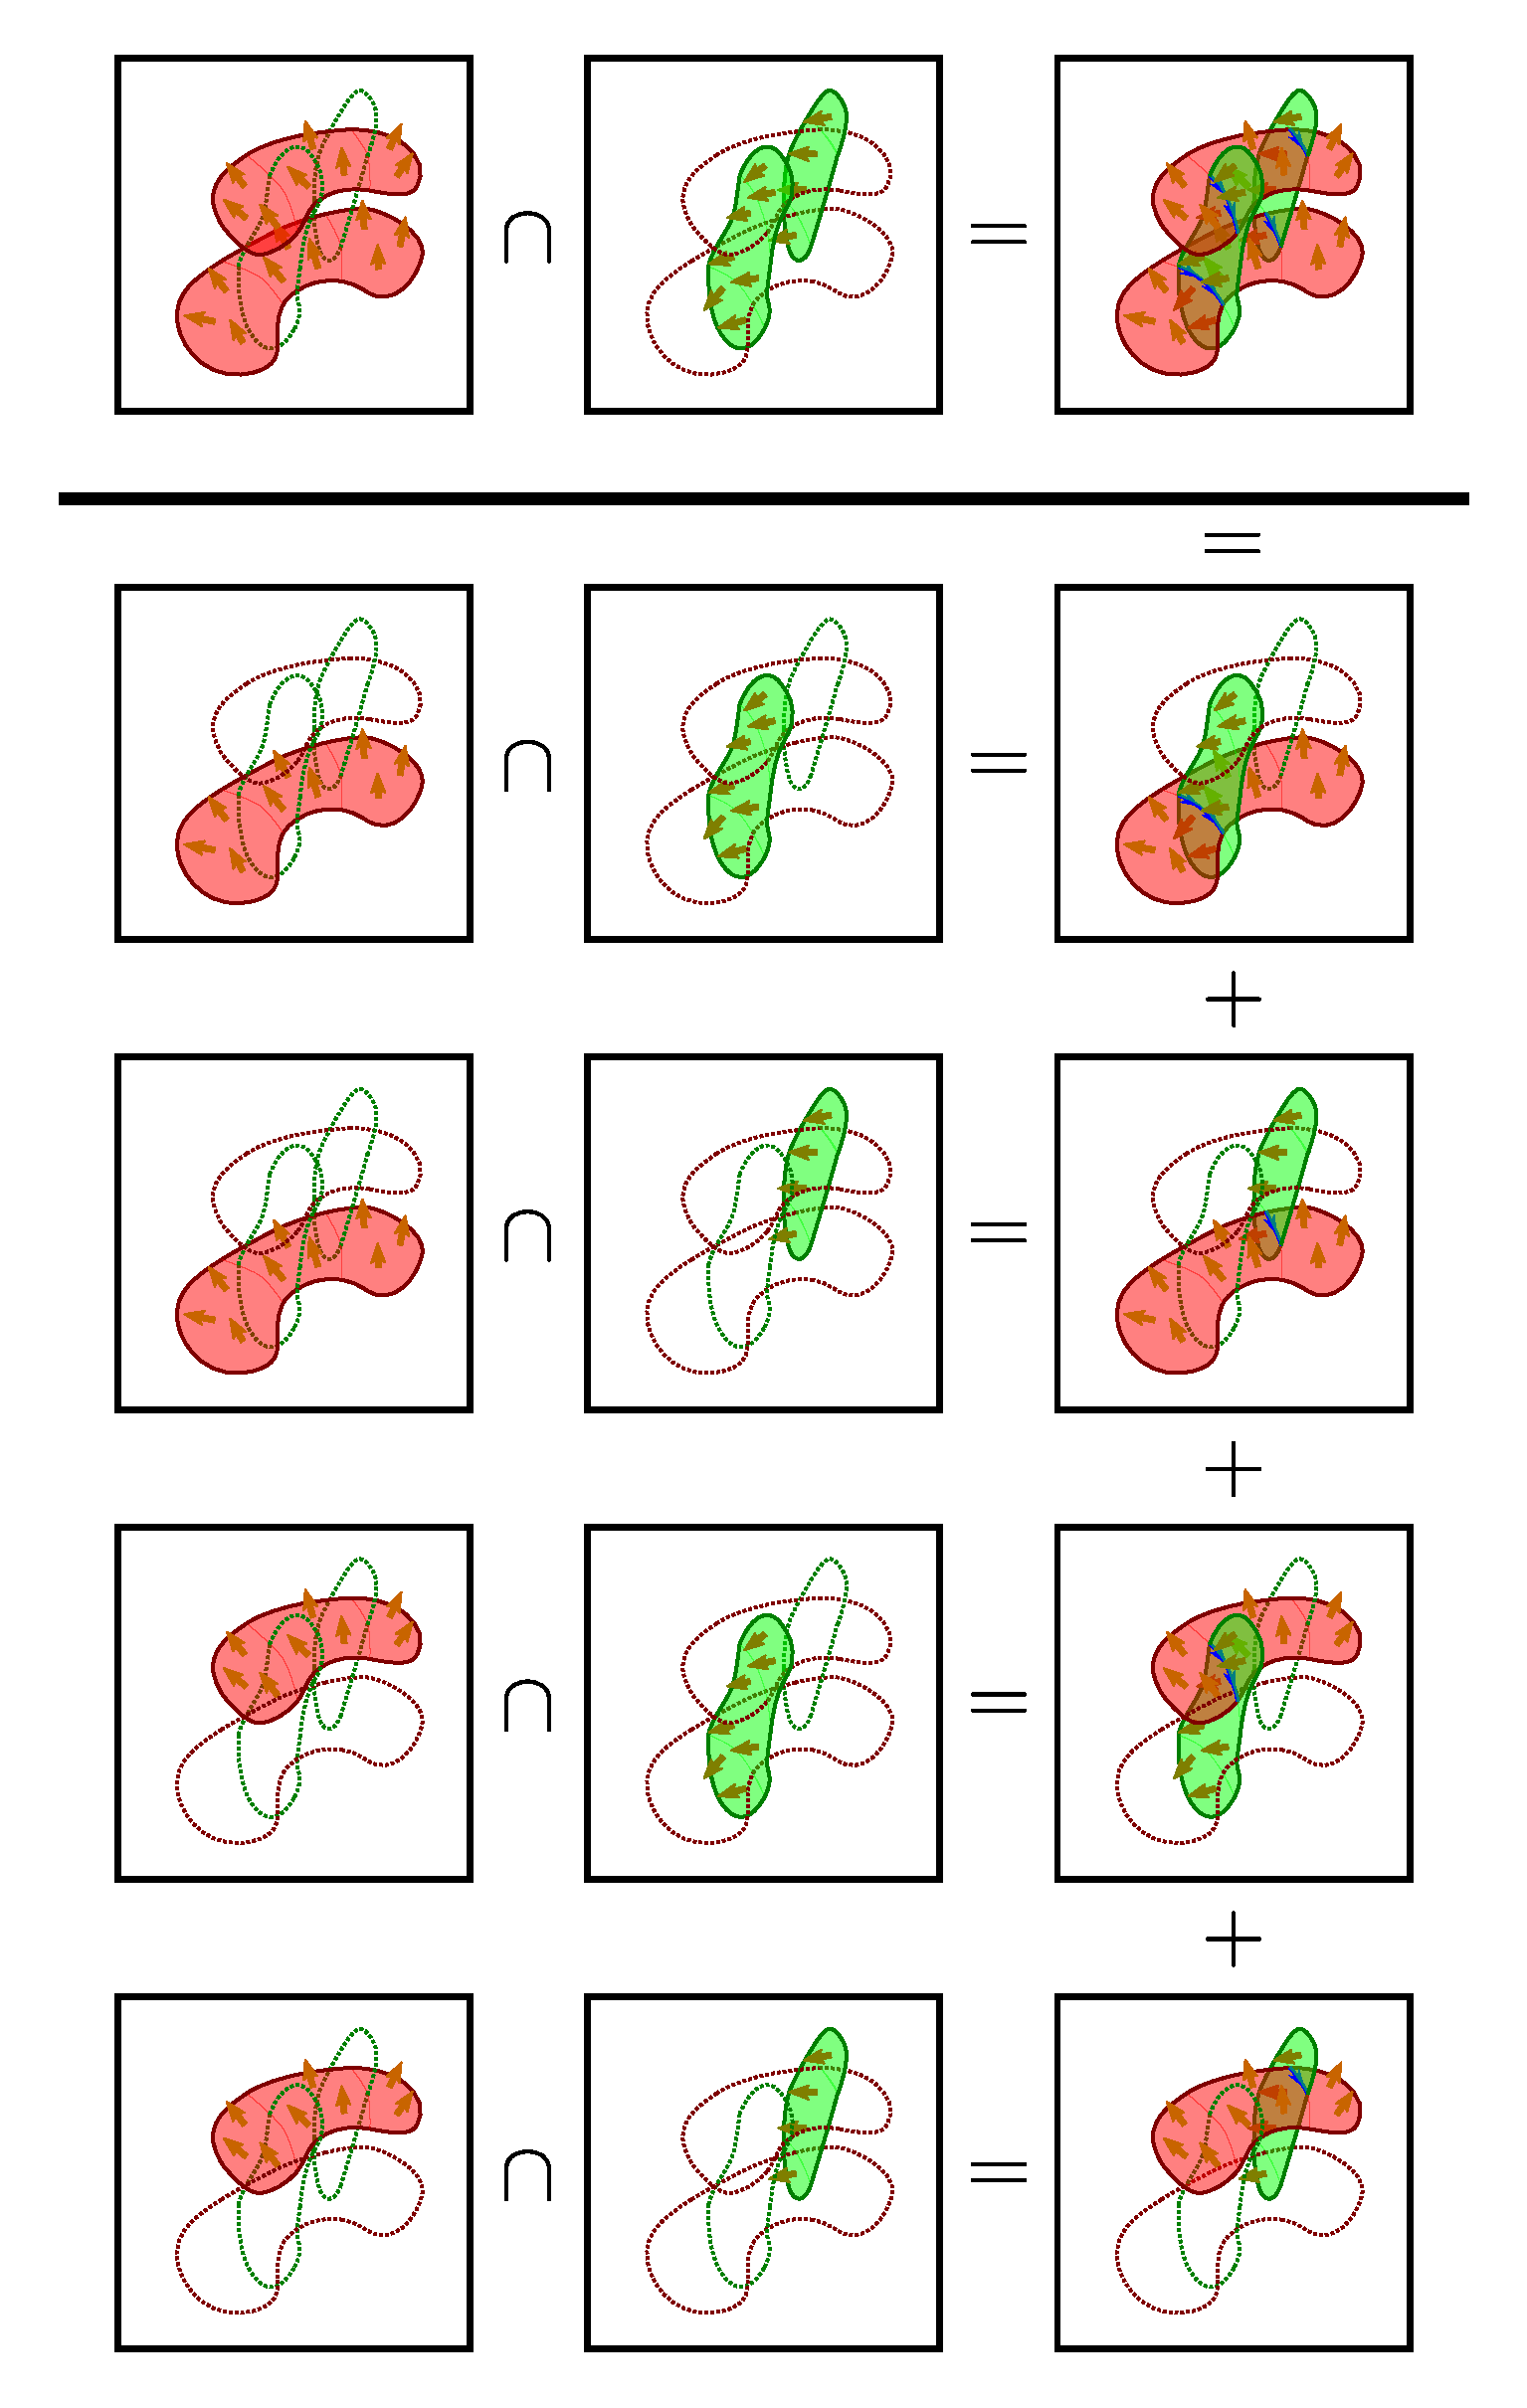
\includegraphics[width = 0.4\textwidth]{Intersections/Surface-surface_intersections/surface_surface_intersection_distributive_law}
}
\end{tabular}
\end{center}

If one surface fails to fully pass through the other surface, then the weight of the intersection path is halved. Surfaces that are embedded inside of other surfaces do contribute any intersection paths unless they enter or leave the other surface. 

Below are examples of surfaces intersecting each other but not fully passing through. Note the bottom example where both surfaces are truncated, so the intersection weight is further halved to \(0.25\).

\begin{center}
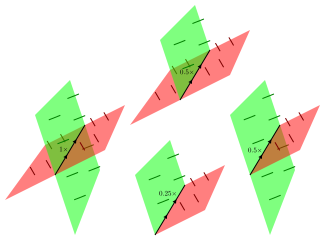
\includegraphics[width = 0.75\textwidth]{Intersections/Surface-surface_intersections/surface_surface_intersection_boundary_case}
\end{center}

Two surfaces that are coincident do not slice through each other and therefore do not intersect. If \(\mathbf{F}_1\) and \(\mathbf{F}_2\) are the same flat surface as depicted below on the left, then these surfaces {\bf do not intersect:} \(\mathbf{F}_1 \times \mathbf{F}_2 = 0\). On the right, the curves where surface \(\mathbf{F}_2\) peels away from \(\mathbf{F}_1\) are intersection curves with weights of \(0.5\).

\begin{center}
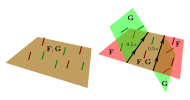
\includegraphics[width = 0.75\textwidth]{Intersections/Surface-surface_intersections/coincident_surfaces}
\end{center}

\begin{tabular}{cc}
\parbox{0.6\textwidth}{
While a surface cannot intersect itself directly as explained above, a surface can still be folded over to explicitly slice through itself as depicted on the right. However, we will soon see that this type of intersection actually does not count, primarily since the intersection cannot be oriented in an objective manner. From a more mathematical perspective, consider the following: Let \(\sigma_1\) and \(\sigma_2\) be two flat surfaces that intersect each other, but with no self intersections that result from folding over. Let multi-surface \(\mathbf{G}\) be comprised of \(\sigma_1\) and \(\sigma_2\):
\[\mathbf{G} = \sigma_1 + \sigma_2\] 
} & \parbox{0.4\textwidth}{
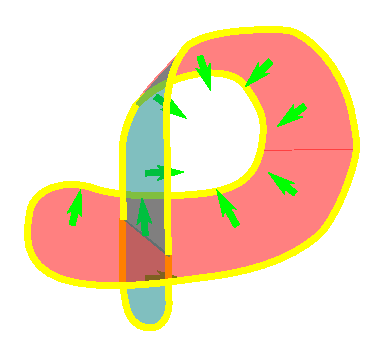
\includegraphics[width = 0.4\textwidth]{Intersections/Surface-surface_intersections/folded_surface_self_intersection}
}
\end{tabular}
The intersection of \(\mathbf{G}\) with itself is: 
\begin{align*}
\mathbf{G} \times \mathbf{G} = (\sigma_1 + \sigma_2) \times (\sigma_1 + \sigma_2) = (\sigma_1 \times \sigma_1) + (\sigma_1 \times \sigma_2) + (\sigma_2 \times \sigma_1) + (\sigma_2 \times \sigma_2)
\end{align*}

We've already established that for surfaces that do not have any self intersections from folding, do not intersect themselves in any other manner, so \(\sigma_1 \times \sigma_1 = 0\) and \(\sigma_2 \times \sigma_2 = 0\). It is also the case that reversing the order of \(\sigma_1\) and \(\sigma_2\) flips the orientation so \(\sigma_2 \times \sigma_1 = -(\sigma_1 \times \sigma_2)\). Therefore: 
\[\mathbf{G} \times \mathbf{G} = 0 + (\sigma_1 \times \sigma_2) + (\sigma_2 \times \sigma_1) + 0 = (\sigma_1 \times \sigma_2) - (\sigma_1 \times \sigma_2) = 0\]

%\begin{center}
%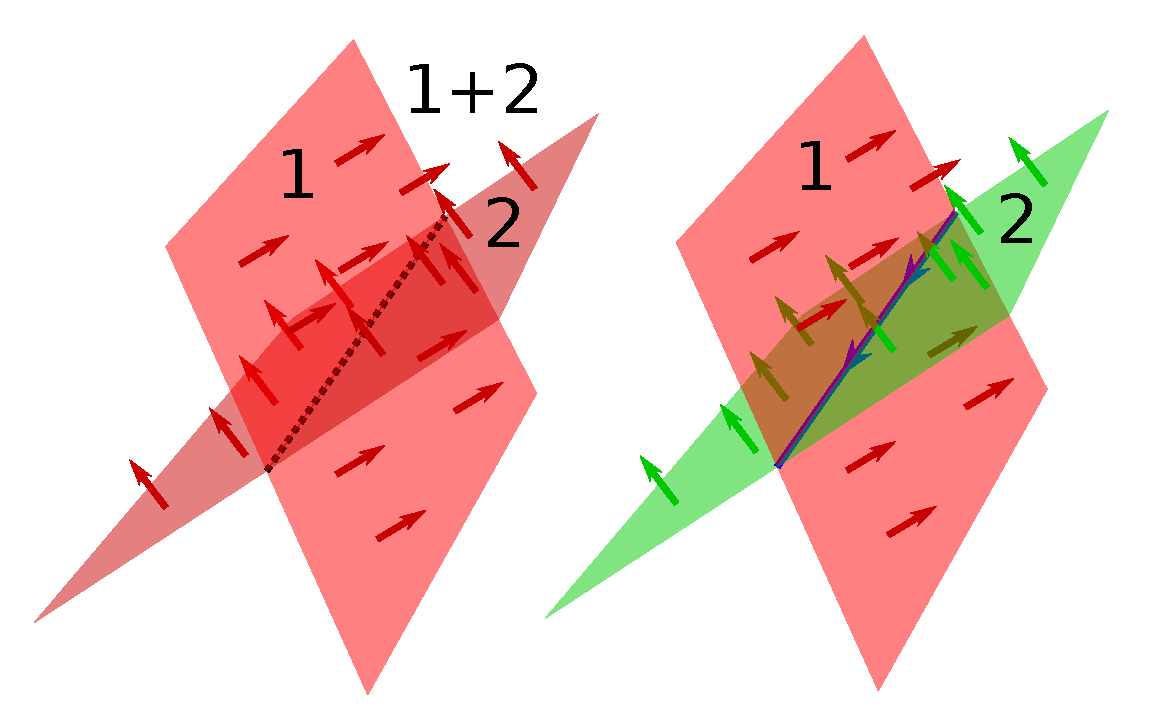
\includegraphics[width = 0.75\textwidth]{Intersections/Surface-surface_intersections/surface_self_intersections}
%\end{center}

In general, the intersection of a multi-surface with itself is always \(0\):

\begin{thm}
\[\mathbf{F} \times \mathbf{F} = 0\]
\end{thm}


Lastly, 3 multi-surface surfaces intersect at a multi-point. Consider \(3\) multi-surfaces \(\mathbf{F}\), \(\mathbf{G}\), and \(\mathbf{H}\). The intersection between \(\mathbf{F}\) and \(\mathbf{G}\) is the multi-path \(\mathbf{F} \times \mathbf{G}\). The intersection between the multi-path \(\mathbf{F} \times \mathbf{G}\) and multi-surface \(\mathbf{H}\) is the multi-point \((\mathbf{F} \times \mathbf{G}) \bullet \mathbf{H}\). This intersection can also be generated by computing the intersection of \(\mathbf{G}\) and \(\mathbf{H}\) first, or the intersection of \(\mathbf{H}\) and \(\mathbf{F}\) first:
\[(\mathbf{F} \times \mathbf{G}) \bullet \mathbf{H} = (\mathbf{G} \times \mathbf{H}) \bullet \mathbf{F} = (\mathbf{H} \times \mathbf{F}) \bullet \mathbf{G}\]
Note that swapping any two surfaces in the above intersections flips the polarity of the intersection point:
\begin{thm}
\begin{align*}
& (\mathbf{F} \times \mathbf{G}) \bullet \mathbf{H} = (\mathbf{G} \times \mathbf{H}) \bullet \mathbf{F} = (\mathbf{H} \times \mathbf{F}) \bullet \mathbf{G} \\ 
= & -(\mathbf{G} \times \mathbf{F}) \bullet \mathbf{H} = -(\mathbf{H} \times \mathbf{G}) \bullet \mathbf{F} = -(\mathbf{F} \times \mathbf{H}) \bullet \mathbf{G}
\end{align*}
\end{thm}

\begin{tabular}{cc}
\parbox{0.5\textwidth}{
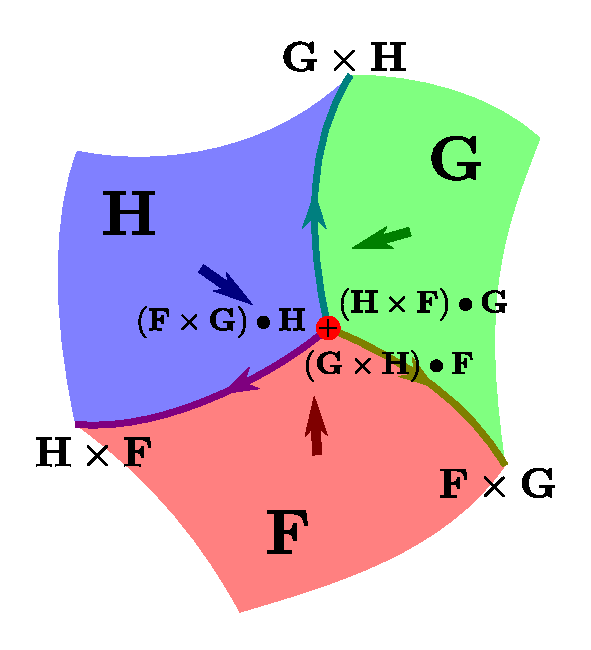
\includegraphics[width = 0.5\textwidth]{Intersections/Surface-surface_intersections/surface_surface_surface_intersections}
} & \parbox{0.5\textwidth}{
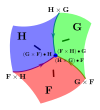
\includegraphics[width = 0.5\textwidth]{Intersections/Surface-surface_intersections/surface_surface_surface_intersections_reversed}
}
\end{tabular}

It was previously noted that a path only ``intersects" a surface when it decisively passes through the surface, and that paths that are embedded within surfaces do not contribute any intersection points. Since the intersection path \(\mathbf{F} \times \mathbf{G}\) is embedded in surfaces \(\mathbf{F}\) and \(\mathbf{G}\), then contrary to intuition, there is no intersection of \(\mathbf{F} \times \mathbf{G}\) with either \(\mathbf{F}\) or \(\mathbf{G}\):
\begin{thm}
\[\mathbf{F} \bullet (\mathbf{F} \times \mathbf{G}) = 0 \quad\quad\quad\text{and}\quad\quad\quad \mathbf{G} \bullet (\mathbf{F} \times \mathbf{G}) = 0\]  
\end{thm}



\section{Surface-volume intersections} 

Given a multi-surface \(\mathbf{F}\) and a multi-volume \(U\), then the intersection between \(\mathbf{F}\) and \(U\) is a multi-surface and is denoted by:

\[\mathbf{F} \cdot U \quad\quad\text{or}\quad\quad \mathbf{F} U \quad\quad\text{or}\quad\quad U \cdot \mathbf{F} \quad\quad\text{or}\quad\quad U \mathbf{F}\]

Given an oriented surface \(\sigma\), and a volume \(\Omega\), then the intersection is the sections of \(\sigma\) that are contained in \(\Omega\). If the weight of \(\Omega\) is negative, then the orientation of the intersection is reversed.  

In the examples below, only sections of the surface that are contained inside a volume are part of the intersection. In the example on the right, because the volume of weight is negative, the orientation is reversed

\begin{center}
\begin{tabular}{cc}
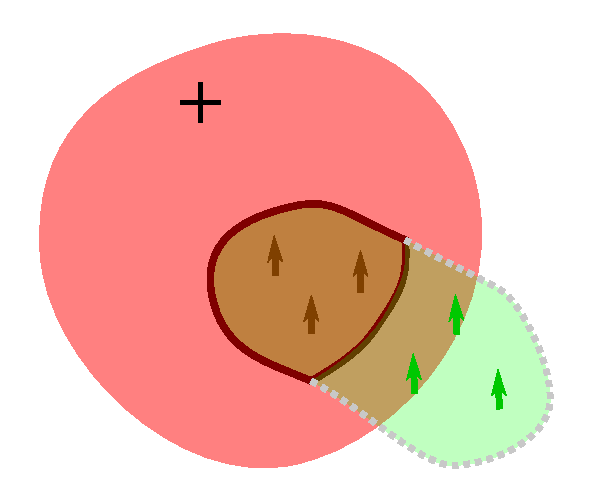
\includegraphics[width = 0.3\textwidth]{Intersections/Surface-volume_intersections/surface_volume_intersections_example_1}
& 
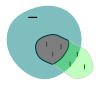
\includegraphics[width = 0.3\textwidth]{Intersections/Surface-volume_intersections/surface_volume_intersections_example_2}
\end{tabular}
\end{center}

If a surface \(\sigma\) with a nonnegative weight of \(w_1\) intersects a volume \(\Omega\) with a weight of \(w_2\) and \(\sigma'\) is the sections of \(\sigma\) that are contained in \(\Omega\), then for each of the \(w_2\) copies of \(\Omega\), \(w_1\) copies of \(\sigma\) are intersecting that copy. The total intersection is \(w_1 \cdot w_2\) copies of \(\sigma'\):
\[(w_1 \sigma) \cdot (w_2 \Omega) = w_1 w_2 \sigma'\] 
If the volume weight \(w_2\) is negative, then both the orientation of \(\sigma'\) and the sign of the weight \(w_1 w_2\) is flipped. 

Given a multi-surface \(\mathbf{F} = w_1\sigma_1 + w_2\sigma_2 + ... + w_N\sigma_N\) and a multi-volume \\ \(U = v_1\Omega_1 + v_2\Omega_2 + ... + v_M\Omega_M\), then the intersection \(\mathbf{F} \cdot U\) is the set of all pairwise intersections of the surfaces and volumes:
\begin{align*}
\mathbf{F} \cdot U = & \left\{\begin{array}{c}
\;\; w_1 v_1 (\sigma_1 \cdot \Omega_1) + w_1 v_2 (\sigma_1 \cdot \Omega_2) + \cdots + w_1 v_M (\sigma_1 \cdot \Omega_M) \\ 
+ w_2 v_1 (\sigma_2 \cdot \Omega_1) + w_2 v_2 (\sigma_2 \cdot \Omega_2) + \cdots + w_2 v_M (\sigma_2 \cdot \Omega_M) \\ 
\vdots \\
+ w_N v_1 (\sigma_N \cdot \Omega_1) + w_N v_2 (\sigma_N \cdot \Omega_2) + \cdots + w_N v_M (\sigma_N \cdot \Omega_M) \\ 
\end{array}\right.
\end{align*}

In general,
\begin{itemize}
\item Given multi-surfaces \(\mathbf{F}_1\) and \(\mathbf{F}_2\), and multi-volume \(U\), then:
\[(\mathbf{F}_1 + \mathbf{F}_2) \cdot U = \mathbf{F}_1 \cdot U + \mathbf{F}_2 \cdot U\] 
\item Given multi-surface \(\mathbf{F}\), multi-volume \(U\), and some real number \(c\), then:
\[(c\mathbf{F}) \cdot U = c(\mathbf{F} \cdot U)\]
\item Given multi-surface \(\mathbf{F}\), and multi-volumes \(U_1\) and \(U_2\), then:
\[\mathbf{F} \cdot (U_1 + U_2) = \mathbf{F} \cdot U_1 + \mathbf{F} \cdot U_2\] 
\item Given multi-surface \(\mathbf{F}\), multi-volume \(U\), and some real number \(c\), then:
\[\mathbf{F} \cdot (cU) = c(\mathbf{F} \cdot U)\]
\end{itemize}

In the example below, the multi-volume \(U\) consists of three volumes. Two of the volumes have a weight of \(+1\) and are overlapping, and the remaining separate volume has a weight of \(-1\). The multi-path \(\mathbf{F}\) consists of a single surface that slices through all of the volumes. Outside of all of the volumes, the surface is not part of the intersection. Where the surface is inside a single volume with a weight of \(+1\), the intersection surface from \(\mathbf{F} \cdot U\) has a weight of \(+1\). Where the surface is inside the overlap between the volumes with a weight of \(+1\), then each volume contributes a copy of the intersection to \(\mathbf{F} \cdot U\) so the weight of the surface in \(\mathbf{F} \cdot U\) is \(+2\). Where the surface is inside the volume with a weight of \(-1\), the orientation of the intersection is reversed.  

\begin{center}
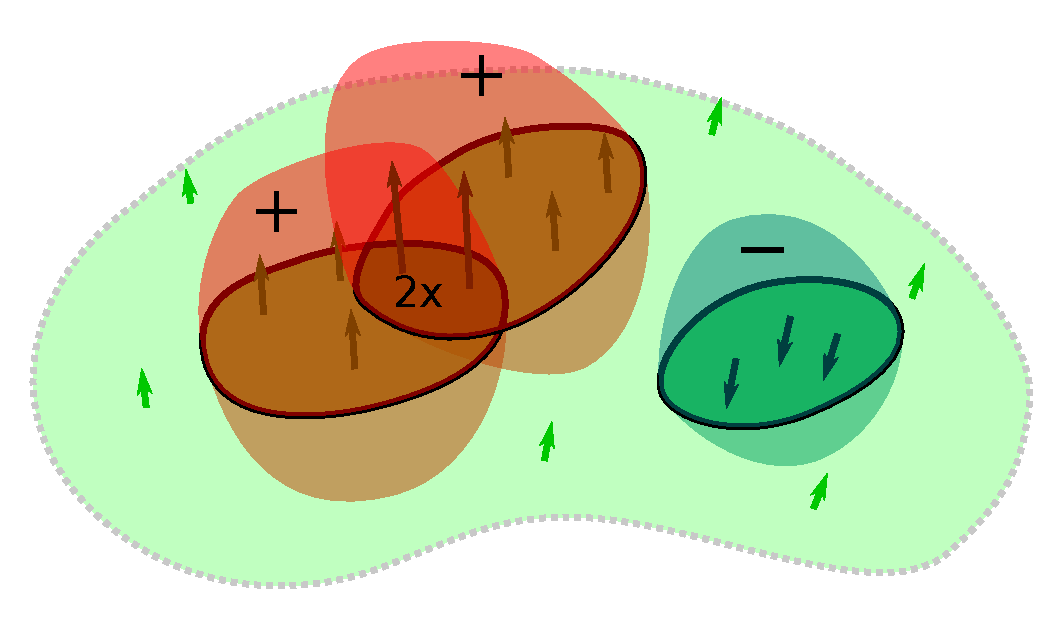
\includegraphics[width = 0.75\textwidth]{Intersections/Surface-volume_intersections/surface_volume_intersections_example_3}
\end{center}

\begin{tabular}{cc}
\parbox{0.5\textwidth}{
If a surface \(\sigma\) is on the surface of volume \(\Omega\), then the intersection is \(\sigma\) with a weight of \(+0.5\) as depicted on the right.
} & \parbox{0.5\textwidth}{
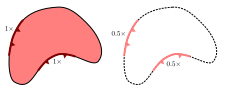
\includegraphics[width = 0.5\textwidth]{Intersections/Surface-volume_intersections/surface_volume_intersection_boundary_case}
}
\end{tabular}





\section{Volume-volume intersections}

Given two multi-volumes \(U_1\) and \(U_2\), then the intersection between \(U_1\) and \(U_2\) is a multi-volume and is denoted by:

\[U_1 \cdot U_1 \quad\quad\text{or}\quad\quad U_1 U_2\]

Given volumes \(\Omega_1\) and \(\Omega_2\), then the intersection is the sections of \(\Omega_1\) and \(\Omega_2\) that overlap. 

If a volume \(\Omega_1\) with a weight of \(w_1\) intersects a volume \(\Omega_2\) with a weight of \(w_2\) and \(\Omega'\) is the sections of \(\Omega_1\) and \(\Omega_2\) that overlap, then for each of the \(w_2\) copies of \(\Omega_2\), \(w_1\) copies of \(\Omega_1\) are intersecting that copy. The total intersection is \(w_1 \cdot w_2\) copies of \(\Omega'\):
\[(w_1\Omega_1) \cdot (w_2\Omega_2) = w_1 w_2 \Omega'\] 

Given multi-volumes \(U_1 = w_1\Omega_1 + w_2\Omega_2 + ... + w_N\Omega_N\) and \\ \(U_2 = v_1\Phi_1 + v_2\Phi_2 + ... + v_M\Phi_M\), then the intersection \(U_1 \cdot U_2\) is the set of all pairwise intersections of the volumes:
\begin{align*}
U_1 \cdot U_2 = & \left\{\begin{array}{c}
\;\; w_1 v_1 (\Omega_1 \cdot \Phi_1) + w_1 v_2 (\Omega_1 \cdot \Phi_2) + \cdots + w_1 v_M (\Omega_1 \cdot \Phi_M) \\ 
+ w_2 v_1 (\Omega_2 \cdot \Phi_1) + w_2 v_2 (\Omega_2 \cdot \Phi_2) + \cdots + w_2 v_M (\Omega_2 \cdot \Phi_M) \\ 
\vdots \\
+ w_N v_1 (\Omega_N \cdot \Phi_1) + w_N v_2 (\Omega_N \cdot \Phi_2) + \cdots + w_N v_M (\Omega_N \cdot \Phi_M) \\ 
\end{array}\right.
\end{align*}

In general,
\begin{itemize}
\item Given multi-volumes \(U_1\), \(U_2\), and \(V\), then:
\[(U_1 + U_2) \cdot V = U_1 \cdot V + U_2 \cdot V\] 
\item Given multi-volumes \(U\) and \(V\), and some real number \(c\), then:
\[(cU) \cdot V = c(U \cdot V)\]
\item Given multi-volumes \(U\), \(V_1\), and \(V_2\), then:
\[U \cdot (V_1 + V_2) = U \cdot V_1 + U \cdot V_2\] 
\item Given multi-volumes \(U\) and \(V\), and some real number \(c\), then:
\[U \cdot (cV) = c(U \cdot V)\]
\end{itemize}

Some examples of intersecting multi-volumes are shown below. Note that for a specific point \(\mathbf{q}\), that the net number of volumes that contain \(\mathbf{q}\) in the intersection \(U_1 \cdot U_2\) will always be the product of the net number of volumes that contain \(\mathbf{q}\) in each of \(U_1\) and \(U_2\):
\[(U_1 \cdot U_2)(\mathbf{q}) = U_1(\mathbf{q}) \cdot U_2(\mathbf{q})\]

\begin{center}
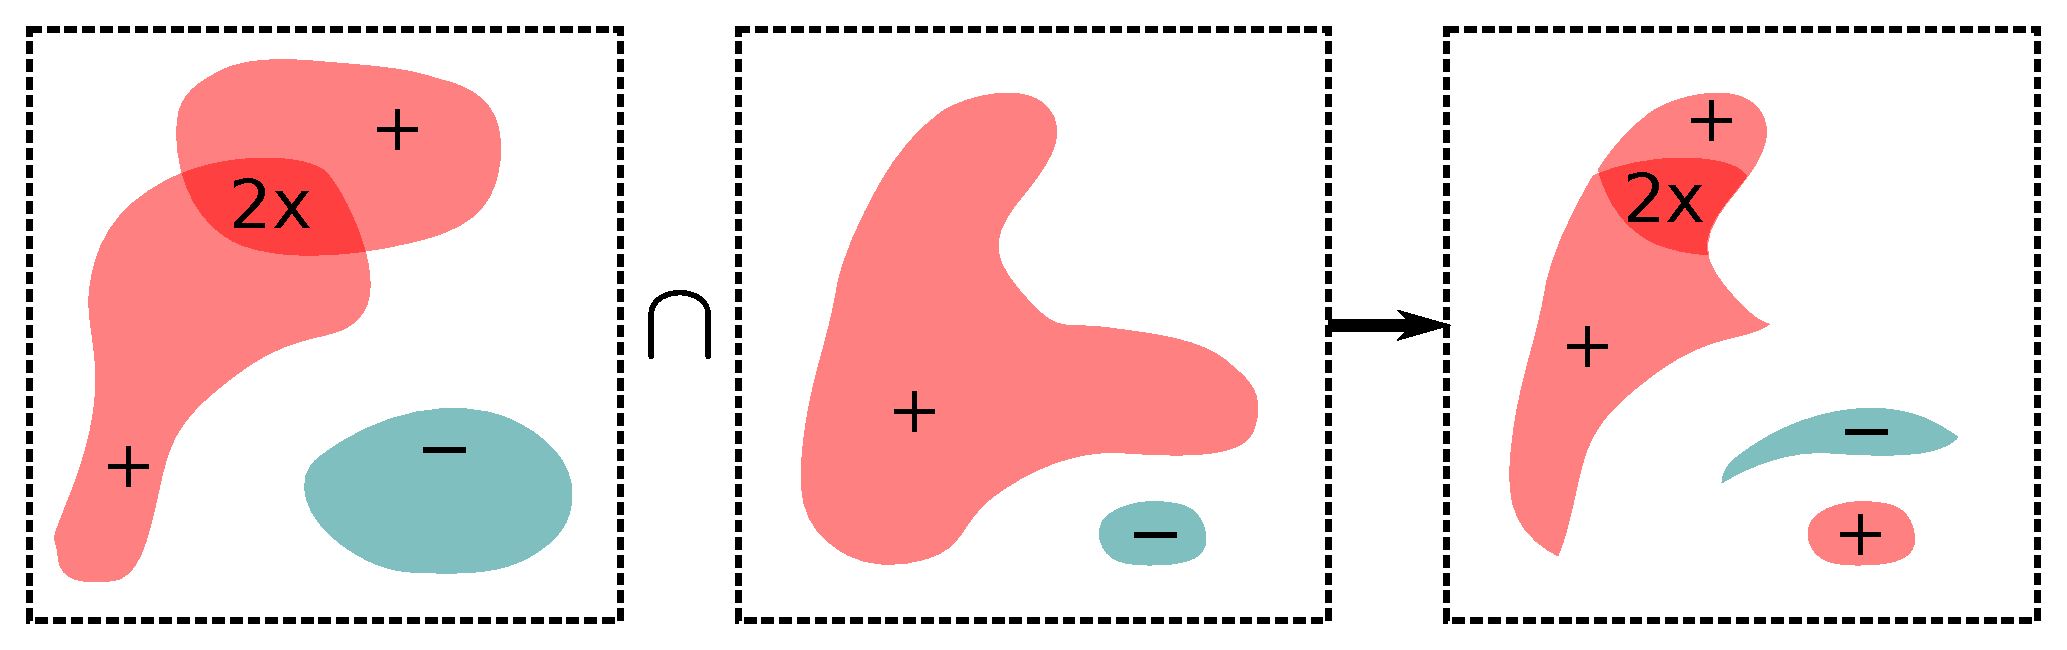
\includegraphics[width = \textwidth]{Intersections/Volume-volume_intersections/volume_volume_intersections_three_panel_example}
\end{center}

\begin{center}
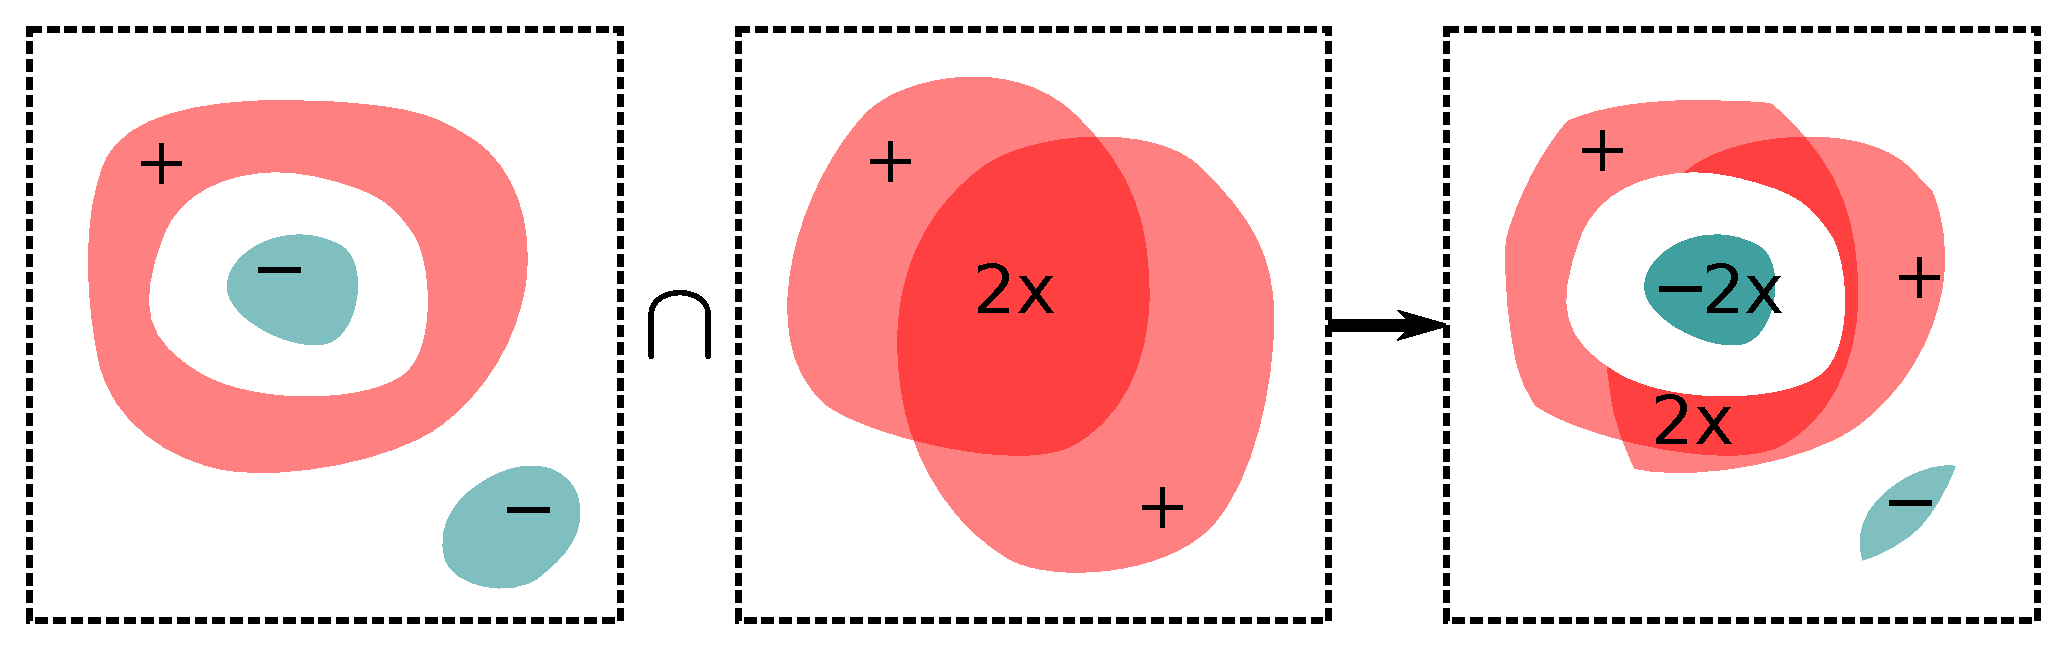
\includegraphics[width = \textwidth]{Intersections/Volume-volume_intersections/volume_volume_intersections_three_panel_example_2}
\end{center}




\section{Intersections that are not being considered}

What about the following other types of intersections? Namely point-point intersections, point-path intersections, point-surface intersections, and path-path intersections? With the exception of point-point intersections, these intersections cannot be oriented as will be discussed: 


\subsection{Point-path intersections}

%\begin{tabular}{cc}
%\parbox{0.5\textwidth}{
%Consider a point \(P\) and an oriented path \(C\) that passes through point \(P\). The intersection of \(P\) with \(C\) consists of just \(P\), but what weight should point \(P\) have in the intersection?
%\[P \cap C = ?P\]
%It may seem obvious that this weight should simply be \(1\), but consider the path \(-C\), which is path \(C\) with the orientation reversed. \(-C\) also passes through point \(P\) so the intersection point \(P\) should also have a weight of \(1\). In fact, the weight of \(P\) in the intersection \(P \cap C\) should be equal to the weight of \(P\) in the intersection \(P \cap (-C)\).
%\begin{align*}
%& P \cap C  
%= ?P 
%= P \cap (-C)
%\end{align*} 
%} & \parbox{0.5\textwidth}{
%\includegraphics[width = 0.5\textwidth]{Intersections/Undefined_intersections/point_path_intersection_contradiction}
%}
%\end{tabular}
%
%\vspace{5mm}
%
%By linearity, the intersection of \(P\) with the union of \(C\) and \(-C\) is the union of the intersection of \(P\) with \(C\) and the intersection of \(P\) with \(-C\):
%\begin{align*}
%& P \cap \Big(C + (-C)\Big) = P \cap C + P \cap (-C)
%\end{align*}
%Since \(P \cap C = P \cap (-C) = ?P\), 
%\begin{align*}
%P \cap C + P \cap (-C) = ?P + ?P = (2?)P
%\end{align*}
%so the intersection of \(P\) with the union of \(C\) and \(-C\) is 
%\[P \cap \Big(C + (-C)\Big) = (2?)P\]
%
%The union of \(C\) and \(-C\) should be nothing: 
%\[C + (-C) = 0\]  
%
%The intersection of \(P\) with nothing is nothing, so
%\[P \cap \Big(C + (-C)\Big) = P \cap 0 = 0\]  
%
%Therefore, 
%\begin{align*}
%& P \cap \Big(C + (-C)\Big) = (2?)P \quad\quad\text{and}\quad\quad P \cap \Big(C + (-C)\Big) = 0 \quad\quad\text{so}\quad\quad (2?)P = 0 \\ 
%& \quad\quad\text{so}\quad\quad ? = 0
%\end{align*}
%so the weight of point \(P\) in the intersections \(P \cap C\) and \(P \cap (-C)\) can only be \(0\). There cannot be any intersection of a point with a path, in a similar manner to how an oriented surface cannot intersect itself as discussed previously.

Why can't point-path intersections be oriented? Let \(P\) be a point and let \(C\) be an oriented path, where point \(P\) lies on \(C\). Let the weights of \(P\) and \(C\) both be \(1\). What weight should point \(P\) have in the intersection? Should the orientation of \(C\) be reversed, the sign of the weight should also be flipped. Now slowly rotate \(C\) around while maintaining the intersection as depicted below. No matter the direction in which \(C\) passes through \(P\) the weight should ideally remain constant as all directions are equal. The question is at what point during the rotation does the sign of the weight flip? The answer is that the weight should always be \(0\), and the intersection does not exist.  

\begin{center}
\includegraphics[width = \textwidth]{Intersections/Undefined_intersections/point_path_intersection_contradiction_2}
\end{center}




\subsection{Point-surface intersections}

%\begin{tabular}{cc}
%\parbox{0.5\textwidth}{
%Consider a point \(P\) and an oriented surface \(\sigma\) that passes through point \(P\). The intersection of \(P\) with \(\sigma\) consists of just \(P\), but what weight should point \(P\) have in the intersection?
%\[P \cap \sigma = ?P\]
%It may seem obvious that this weight should simply be \(1\), but consider the surface \(-\sigma\), which is surface \(\sigma\) with the orientation reversed. \(-\sigma\) also passes through point \(P\) so the intersection point \(P\) should also have a weight of \(1\). In fact, the weight of \(P\) in the intersection \(P \cap \sigma\) should be equal to the weight of \(P\) in the intersection \(P \cap (-\sigma)\).
%\begin{align*}
%& P \cap \sigma  
%= ?P 
%= P \cap (-\sigma)  
%\end{align*} 
%} & \parbox{0.5\textwidth}{
%\includegraphics[width = 0.5\textwidth]{Intersections/Undefined_intersections/point_surface_intersection_contradiction}
%}
%\end{tabular}
%
%\vspace{5mm}
%
%By linearity, the intersection of \(P\) with the union of \(\sigma\) and \(-\sigma\) is the union of the intersection of \(P\) with \(\sigma\) and the intersection of \(P\) with \(-\sigma\):
%\begin{align*}
%& P \cap \Big(\sigma + (-\sigma)\Big) = P \cap \sigma + P \cap (-\sigma)
%\end{align*}
%Since \(P \cap \sigma = P \cap (-\sigma) = ?P\), 
%\begin{align*}
%P \cap \sigma + P \cap (-\sigma) = ?P + ?P = (2?)P  
%\end{align*}
%so the intersection of \(P\) with the union of \(\sigma\) and \(-\sigma\) is 
%\[P \cap \Big(\sigma + (-\sigma)\Big) = (2?)P\]
%
%The union of \(\sigma\) and \(-\sigma\) should be nothing: 
%\[\sigma + (-\sigma) = 0\]
%
%The intersection of \(P\) with nothing is nothing, so
%\[P \cap \Big(\sigma + (-\sigma)\Big) = P \cap 0 = 0\]  
%
%Therefore, 
%\begin{align*}
%& P \cap \Big(\sigma + (-\sigma)\Big) = (2?)P \quad\quad\text{and}\quad\quad P \cap \Big(\sigma + (-\sigma)\Big) = 0 \quad\quad\text{so}\quad\quad (2?)P = 0 \\ 
%& \quad\quad\text{so}\quad\quad ? = 0
%\end{align*}
%so the weight of point \(P\) in the intersections \(P \cap \sigma\) and \(P \cap (-\sigma)\) can only be \(0\). There cannot be any intersection of a point with a surface, in a similar manner to how an oriented surface cannot intersect itself as discussed previously.

Why can't point-surface intersections be oriented? Let \(P\) be a point and let \(\sigma\) be an oriented surface, where point \(P\) lies on \(\sigma\). Let the weights of \(P\) and \(\sigma\) both be \(1\). What weight should point \(P\) have in the intersection? Should the orientation of \(\sigma\) be reversed, the sign of the weight should also be flipped. Now slowly rotate \(\sigma\) around while maintaining the intersection as depicted below. No matter the direction in which \(\sigma\) faces as it passes through \(P\) the weight should ideally remain constant as all directions are equal. The question is at what point during the rotation does the sign of the weight flip? The answer is that the weight should always be \(0\), and the intersection does not exist.  

\begin{center}
\includegraphics[width = \textwidth]{Intersections/Undefined_intersections/point_surface_intersection_contradiction_2}
\end{center}



\subsection{Path-path intersections}

%\begin{tabular}{cc}
%\parbox{0.5\textwidth}{
%Consider two paths \(C_1\) and \(C_2\) that intersect at point \(P\). What weight should point \(P\) have in the intersection?
%\[C_1 \cap C_2 = ?P\]
%It may seem obvious that this weight should simply be \(1\), but consider the path \(-C_2\), which is path \(C_2\) with the orientation reversed. \(-C_2\) also intersects \(C_1\) at point \(P\) so the intersection point \(P\) should also have a weight of \(1\). In fact, the weight of \(P\) in the intersection \(C_1 \cap C_2\) should be equal to the weight of \(P\) in the intersection \(C_1 \cap -C_2\).
%\begin{align*}
%& C_1 \cap C_2  
%= ?P 
%= C_1 \cap (-C_2)
%\end{align*} 
%} & \parbox{0.5\textwidth}{
%\includegraphics[width = 0.5\textwidth]{Intersections/Undefined_intersections/path_path_intersection_contradiction}
%}
%\end{tabular}
%
%\vspace{5mm}
%
%By linearity, the intersection of \(C_1\) with the union of \(C_2\) and \(-C_2\) is the union of the intersection of \(C_1\) with \(C_2\) and the intersection of \(C_1\) with \(-C_2\):
%\begin{align*}
%& C_1 \cap \Big(C_2 + (-C_2)\Big) = C_1 \cap C_2 + C_1 \cap (-C_2)
%\end{align*}
%Since \(C_1 \cap C_2 = C_1 \cap (-C_2) = ?P\), 
%\begin{align*}
% C_1 \cap C_2 + C_1 \cap (-C_2) = ?P + ?P = (2?)P 
%\end{align*}
%so the intersection of \(C_1\) with the union of \(C_2\) and \(-C_2\) is 
%\[C_1 \cap \Big(C_2 + (-C_2)\Big) = (2?)P\]
%
%The union of \(C_2\) and \(-C_2\) should be nothing: 
%\[C_2 + (-C_2) = 0\]
%
%The intersection of \(C_1\) with nothing is nothing, so
%\[C_1 \cap \Big(C_2 + (-C_2)\Big) = C_1 \cap 0 = 0\]  
%
%Therefore, 
%\begin{align*}
%& C_1 \cap \Big(C_2 + (-C_2)\Big) = (2?)P \quad\quad\text{and}\quad\quad C_1 \cap \Big(C_2 + (-C_2)\Big) = 0 \quad\quad\text{so}\quad\quad (2?)P = 0 \\ 
%& \quad\quad\text{so}\quad\quad ? = 0
%\end{align*}
%so the weight of point \(P\) in the intersections \(C_1 \cap C_2\) and \(C_1 \cap (-C_2)\) can only be \(0\). There cannot be any intersection of a path with a path, in a similar manner to how an oriented surface cannot intersect itself as discussed previously.

Why can't path-path intersections be oriented? Let \(C_1\) and \(C_2\) be oriented paths that intersect at point \(P\). Let the weights of \(C_1\) and \(C_2\) both be \(1\). What weight should point \(P\) have in the intersection? Should the orientation of \(C_1\) xor \(C_2\) be reversed, the sign of the weight should also be flipped. Now slowly rotate \(C_2\) around while maintaining the intersection as depicted below. Also, at no point during the rotation \(C_2\) will have the same direction of \(C_1\). No matter the direction in which \(C_2\) intersects \(C_1\) the weight should ideally remain constant as all directions are equal (except if \(C_1\) and \(C_2\) share the same direction). The question is at what point during the rotation does the sign of the weight flip? The answer is that the weight should always be \(0\), and the intersection does not exist.  

\begin{center}
\includegraphics[width = \textwidth]{Intersections/Undefined_intersections/path_path_intersection_contradiction_2}
\end{center}



\section{Summary}

A summary of the notations used for various intersections is given below:

\vspace{5mm}

\begin{tabular}{|c||c|c|c|c|}
\hline
Intersections & point \(\rho_2\) \red{\{0\}} & path \(\mathbf{J}_2\) \red{\{1\}} & surface \(\mathbf{F}_2\) \red{\{2\}} & volume \(U_2\) \red{\{3\}} \\
\hline
\hline
point \(\rho_1\) \red{\{0\}} & 
N/A \red{\{-3\}} & 
N/A \red{\{-2\}} & 
N/A \red{\{-1\}} & 
point \(\rho_1 \cdot U_2\) \red{\{0\}} \\ 
\hline
path \(\mathbf{J}_1\) \red{\{1\}} & 
N/A \red{\{-2\}} & 
N/A \red{\{-1\}} & 
point \(\mathbf{J}_1 \bullet \mathbf{F}_2\) \red{\{0\}} & 
path \(\mathbf{J}_1 \cdot U_2\) \red{\{1\}} \\ 
\hline
surface \(\mathbf{F}_1\) \red{\{2\}} & 
N/A \red{\{-1\}} & 
point \(\mathbf{F}_1 \bullet \mathbf{J}_2\) \red{\{0\}} & 
path \(\mathbf{F}_1 \times \mathbf{F}_2\) \red{\{1\}} & 
surface \(\mathbf{F}_1 \cdot U_2\) \red{\{2\}} \\ 
\hline
volume \(U_1\) \red{\{3\}} & 
point \(U_1 \cdot \rho_2\) \red{\{0\}} & 
path \(U_1 \cdot \mathbf{J}_2\) \red{\{1\}} & 
surface \(U_1 \cdot \mathbf{F}_2\) \red{\{2\}} & 
volume \(U_1 \cdot U_2\) \red{\{3\}} \\
\hline
\end{tabular}

\vspace{5mm}

In \red{red} is indicated the ``dimensionality" of the multi-structure. Points have \(0\) dimensions; paths have \(1\) dimension; surfaces have \(2\) dimensions; and volumes have \(3\) dimensions. The number of dimensions of the intersection is the sum of the dimensions minus \(3\). When the resultant number of dimensions is less than \(0\), the intersection does not exist.



\chapter{Boundaries}

Now will be discussed are the multi-structures that constitute the boundaries of other multi-structures. There will be the endpoints of multi-paths, the boundaries of multi-surfaces, and the surfaces of multi-volumes. Throughout the discussion the symbol ``\(\nabla\)", referred to as a ``nabla", will see frequent use. One possible interpretation of \(\nabla\) is:

\[\nabla = \text{``the inwards oriented surface of reality"}\]

By ``inwards oriented surface of reality", reality is in ``front" of \(\nabla\), and ``un-reality" is behind \(\nabla\). \(\nabla\) {\bf is not an actual 2D surface}, but this interpretation is useful regardless.



\section{Point totals}

Given a multi-point \(\rho\), the total sum of the weights of all of the points that comprise \(\rho\) is denoted by:

\[\int \rho\]

The elongated \(S\), \(\int\), literally stands for sum.

If \(\rho = w_1 P_1 + w_2 P_2 + ... + w_N P_N\) where \(P_1\), \(P_2\), ..., \(P_N\) are single points, then
\[\int \rho = \int (w_1 P_1 + w_2 P_2 + ... + w_N P_N) = w_1 + w_2 + ... + w_N\]

\begin{center} 
\includegraphics[width = 0.5\textwidth]{Point_totals/multi-point_sums}
\end{center}




\section{Path endpoints}

Given a multi-path \(\mathbf{J}\), the ``endpoints" of \(\mathbf{J}\) is a multi-point that is denoted by:

\[\nabla \bullet \mathbf{J}\]

Given an oriented path \(C\), let \(P_0\) be the starting point of \(C\), and let \(P_1\) be the finishing point of \(C\). The multi-point that is the endpoints of \(C\) consists of \(P_0\) with a weight of \(+1\) and \(P_1\) with a weight of \(-1\):

\[\nabla \bullet C = P_0 - P_1\]

\begin{center}
\includegraphics[width = \textwidth]{Boundaries/Path_endpoints/path_endpoint_examples}
\end{center}

The endpoints of a multi-path is the sum of the endpoints of all of the constituent paths:
\[\nabla \bullet (w_1 C_1 + w_2 C_2 + ... + w_N C_N)
= w_1(\nabla \bullet C_1) + w_2(\nabla \bullet C_2) + ... + w_N(\nabla \bullet C_N)\]

\begin{center}
\includegraphics[width = \textwidth]{Boundaries/Path_endpoints/path_endpoint_examples_2}
\end{center}


\begin{thm}
It should be noted that a closed loop has a net endpoint of \(0\). If multi-path \(\mathbf{J}\) consists of only closed loops, then \(\nabla \bullet \mathbf{J} = 0\). 
\end{thm}

It has already been established that paths are not allowed to extend to infinity, hence every starting point must be paired with a finishing point. Starting points have weights of \(+1\), while finishing points have weights of \(-1\). This means that for an arbitrary multi-path \(\mathbf{J}\), that the sum of all of the endpoint weights is \(0\): 
\begin{thm}
For any multi-path \(\mathbf{J}\),
\[\int (\nabla \bullet \mathbf{J}) = 0\] 
\end{thm}

\begin{tabular}{cc}
\parbox{0.5\textwidth}{
A logical question is why the notation \(\nabla \bullet \mathbf{J}\) is used to denote the endpoints of multi-path \(\mathbf{J}\). The notation \(\mathbf{F} \bullet \mathbf{J}\) denotes the intersection of multi-path \(\mathbf{J}\) with multi-surface \(\mathbf{F}\) in the preferred direction. With \(\nabla\) denoting the inwards oriented surface of reality, \(\nabla \bullet \mathbf{J}\) consists of points where \(\mathbf{J}\) enters reality with a weight of \(+1\), and leaves reality with a weight of \(-1\). This is illustrated on the right.
} & \parbox{0.4\textwidth}{
\includegraphics[width = 0.4\textwidth]{Boundaries/Path_endpoints/path_surface_intersections_and_path_endpoints}
}
\end{tabular}




\section{Surface boundaries}

Given a multi-surface \(\mathbf{F}\), the ``boundaries" of \(\mathbf{F}\) is a multi-path that is denoted by: 

\[\nabla \times \mathbf{F}\]

Given an oriented surface \(\sigma\), the boundary of \(\sigma\) is its {\bf counterclockwise} oriented boundary. The counterclockwise orientation is the orientation that traverses the boundary in a counterclockwise direction when the front of the surface is visible. 

More exactly, the counterclockwise orientation is determined as follows. Position your view point so that the front of \(\sigma\) is visible. When \(\sigma\) is on your right, the boundary is oriented towards you. This is demonstrated in the rightmost example below where the boundary circles the hole in a clockwise direction.

\begin{center}
\includegraphics[width = \textwidth]{Boundaries/Surface_boundaries/surface_boundary_examples}
\end{center}

The counterclockwise boundary of a multi-surface is the sum of the boundaries of all of the constituent surfaces:
\[\nabla \times (w_1 \sigma_1 + w_2 \sigma_2 + ... + w_N \sigma_N)
= w_1(\nabla \times \sigma_1) + w_2(\nabla \times \sigma_2) + ... + w_N(\nabla \times \sigma_N)\]

\begin{center}
\includegraphics[width = \textwidth]{Boundaries/Surface_boundaries/surface_boundary_examples_2}
\end{center}

\begin{thm}
It should be noted that a closed surface (a bubble) has no boundaries. If multi-surface \(\mathbf{F}\) consists of only closed surfaces (bubbles), then \(\nabla \times \mathbf{F} = 0\). 
\end{thm}

The boundaries of surfaces do not abruptly end, and must be closed loops. The counterclockwise boundaries do not have end points. 
\begin{thm}
For any multi-surface \(\mathbf{F}\), 
\[\nabla \bullet (\nabla \times \mathbf{F}) = 0\]
\end{thm}

\begin{tabular}{cc}
\parbox{0.5\textwidth}{
A logical question is why the notation \(\nabla \times \mathbf{F}\) is used to denote the counterclockwise boundary of multi-surface \(\mathbf{F}\). The notation \(\mathbf{G} \times \mathbf{F}\) denotes the intersection of multi-surface \(\mathbf{G}\) with multi-surface \(\mathbf{F}\), with \(\mathbf{F}\) as the \(2^\text{nd}\) surface. With \(\nabla\) denoting the inwards oriented surface of reality, \(\nabla \times \mathbf{F}\) consists of the path where \(\mathbf{F}\) slices into and out of reality. This is illustrated on the right.
} & \parbox{0.5\textwidth}{
\includegraphics[width = 0.5\textwidth]{Boundaries/Surface_boundaries/right_hand_rule_for_boundaries}
}
\end{tabular}




\section{Volume surfaces}

Given a multi-volume \(U\), the ``surfaces" of \(U\) is a multi-surface that is denoted by: 

\[\nabla U\]

Given a volume \(\Omega\), the surface of \(\Omega\) is {\bf inwards-oriented}. 

\begin{center}
\includegraphics[width = \textwidth]{Boundaries/Volume_inwards_oriented_surfaces/volume_surface_examples}
\end{center}

The inwards oriented surface of a multi-volume is the sum of the inwards oriented surfaces of all of the constituent volumes:
\[\nabla (w_1 \Omega_1 + w_2 \Omega_2 + ... + w_N \Omega_N)
= w_1(\nabla \Omega_1) + w_2(\nabla \Omega_2) + ... + w_N(\nabla \Omega_N)\]

In the examples depicted below, the ``inwards oriented surfaces" of volumes that have a negative weight are in fact oriented outwards.

\begin{center}
\includegraphics[width = \textwidth]{Boundaries/Volume_inwards_oriented_surfaces/volume_surface_examples_2}
\end{center}

The surfaces of volumes are bubbles that have no boundaries. 
\begin{thm}
For any multi-volume \(U\), 
\[\nabla \times (\nabla U) = 0\]
\end{thm} 

\begin{tabular}{cc}
\parbox{0.5\textwidth}{
A logical question is why the notation \(\nabla U\) is used to denote the inwards oriented surface of multi-volume \(U\). The notation \(\mathbf{F} U\) denotes the intersection of multi-volume \(U\) with multi-surface \(\mathbf{F}\). With \(\nabla\) denoting the inwards oriented surface of reality, \(\nabla U\) consists of the surface where \(U\) pushes into and out of reality. The surface is inwards oriented since \(\nabla\) is inwards oriented. This is illustrated on the right.
} & \parbox{0.3\textwidth}{
\includegraphics[width = 0.3\textwidth]{Boundaries/Volume_inwards_oriented_surfaces/surface_volume_intersections_and_volume_surfaces}
}
\end{tabular}



\section{Summary}

A summary of the notations used for the different boundaries is given below. In addition, we have observed that the boundaries have no boundaries themselves.

\begin{center}
\begin{tabular}{|c||c|c|c|}
\hline
multi-structure & boundary & orientation & no boundary of the boundary property \\
\hline
\hline
point \(\rho\) \red{\{0\}} &
N/A \red{\{-1\}} &
N/A & 
N/A \\ 
\hline 
path \(\mathbf{J}\) \red{\{1\}} & 
point \(\nabla \bullet \mathbf{J}\) \red{\{0\}} & 
positive start, negative end &
\(\int (\nabla \bullet \mathbf{J}) = 0\) \\
\hline
surface \(\mathbf{F}\) \red{\{2\}} & 
path \(\nabla \times \mathbf{F}\) \red{\{1\}} & 
counterclockwise &
\(\nabla \bullet (\nabla \times \mathbf{F}) = 0\) \\
\hline
volume \(U\) \red{\{3\}} & 
surface \(\nabla U\) \red{\{2\}} & 
inwards-oriented & 
\(\nabla \times (\nabla U) = 0\) \\
\hline
\end{tabular}
\end{center}

In \red{red} is indicated the ``dimensionality" of the multi-structure. Points have \(0\) dimensions; paths have \(1\) dimension; surfaces have \(2\) dimensions; and volumes have \(3\) dimensions. The number of dimensions of the boundary is the number of dimensions minus \(1\). When the resultant number of dimensions is less than \(0\), the boundary does not exist.





\chapter{Closed loops and surfaces}

\section{Balanced multi-points}

Consider a multi-path \(\mathbf{J}\). Since no paths extend to infinity, every starting point, which has a weight of \(+1\), is paired with a finishing point, which has a weight of \(-1\). The total weight of all the endpoints is \(0\):
\[\int (\nabla \bullet \mathbf{J}) = 0\]

If multi-point \(\rho\) has a net total weight of \(0\), then \(\rho\) will be referred to as being a {\bf balanced multi-point}.

\[\rho \quad\text{ is balanced if and only if }\quad \int \rho = 0\]

While the endpoints of any multi-path are balanced, it is also the case that given an arbitrary balanced multi-point \(\rho\), that there exists some multi-path whose endpoints are \(\rho\):

\begin{thm}
If multi-point \(\rho\) is such that \(\int \rho = 0\) then there exists a multi-path \(\mathbf{J}\) such that \(\nabla \bullet \mathbf{J} = \rho\)
\end{thm}

This multi-path \(\mathbf{J}\) can be created by drawing oriented paths in a ``dot-to-dot" fashion starting from points with positive weight and ending on points with negative weight. The resultant multi-path is {\bf not unique}, as there are infinitely many ways to link the endpoints. The image below shows a balanced multi-point and two possible multi-paths whose endpoints are the given balanced multi-point. 

\begin{center}
\includegraphics[width = \textwidth]{Boundaries/Path_endpoints/dot-to-dot}
\end{center}




\section{Closed loops}

Consider a multi-surface \(\mathbf{F}\). The boundary of surfaces have no endpoints, and are ``closed loops":
\[\nabla \bullet (\nabla \times \mathbf{F}) = 0\]    

If multi-path \(\mathbf{J}\) has no endpoints, then \(\mathbf{J}\) will be referred to as being a {\bf multi-loop}.

\[\mathbf{J} \quad\text{ is a multi-loop (closed loop) if and only if }\quad \nabla \bullet \mathbf{J} = 0\]

While the boundary of any multi-surface is a multi-loop, it is also the case that given an arbitrary multi-loop \(\mathbf{J}\), that there exists some multi-surface whose boundary is \(\mathbf{J}\):

\begin{thm}
If multi-path \(\mathbf{J}\) is such that \(\nabla \bullet \mathbf{J} = 0\) then there exists a multi-surface \(\mathbf{F}\) such that \(\nabla \times \mathbf{F} = \mathbf{J}\)
\end{thm}

This multi-surface \(\mathbf{F}\) can be created by filling each loop with a surface that has the correct orientation. This filling can be done by starting at a specific point on the loop, and then ``extending" a film be following the loop. The resultant multi-surface is {\bf not unique}, as there are infinitely many ways to fill a loop. The image below shows a multi-loop and two possible multi-surfaces whose boundaries are the given multi-loop. 

\begin{center}
\includegraphics[width = \textwidth]{Boundaries/Surface_boundaries/surface_filling}
\end{center}

Below are examples of filling in more exotic loops with surfaces. On the left, there is the trefoil knot, while on the right, there is a helical coil. Helical coils have important applications in electronics and electromagnetism. 

\begin{center}
\includegraphics[width = 0.75\textwidth]{Boundaries/Surface_boundaries/exotic_surface_filling_examples}
\end{center}




\section{Closed surfaces}

Consider a multi-volume \(U\). The surfaces of volumes have no boundaries, and are ``closed surfaces/bubbles":
\[\nabla \times (\nabla U) = 0\]    

If multi-surface \(\mathbf{F}\) has no boundary, then \(\mathbf{F}\) will be referred to as being a {\bf multi-bubble}.

\[\mathbf{F} \quad\text{ is a multi-bubble (closed surface) if and only if }\quad \nabla \times \mathbf{F} = 0\]

While the surface of any multi-volume is a multi-bubble, it is also the case that given an arbitrary multi-bubble \(\mathbf{F}\), that there exists {\bf a unique} multi-volume whose surface is \(\mathbf{F}\):

\begin{thm}
If multi-surface \(\mathbf{F}\) is such that \(\nabla \times \mathbf{F} = 0\)
then there exists a {\bf unique} multi-volume \(U\) such that \(\nabla U = \mathbf{F}\)
\end{thm}

This multi-volume \(U\) can be created by filling each of the bubbles with a volume that has the correct weight (outwards oriented bubbles are filled with negative volume). The resultant multi-volume is {\bf unique}, as there is only one way to fill a bubble, unlike filling a boundary or connecting two points.



\begin{tabular}{cc}
\parbox{0.5\textwidth}{
Given a multi-loop \(\mathbf{J}\) and a multi-bubble \(\mathbf{F}\), the net number of times loop \(\mathbf{J}\) enters bubble \(\mathbf{F}\) is equal to the net number of times loop \(\mathbf{J}\) leaves bubble \(\mathbf{F}\). Entrance points have an equal and opposite weight to exit points. This means that the net total of all the intersection points is \(0\): \(\int \mathbf{J} \bullet \mathbf{F} = 0\). 

\begin{thm}
If multi-path \(\mathbf{J}\) is such that \(\nabla \bullet \mathbf{J} = 0\), 

and multi-surface \(\mathbf{F}\) is such that \(\nabla \times \mathbf{F} = 0\), 

then \(\int (\mathbf{J} \bullet \mathbf{F}) = 0\)
\end{thm}
} & \parbox{0.5\textwidth}{
\includegraphics[width = 0.5\textwidth]{Intersections/Path-surface_intersections/closed_surface_and_closed_path}
}
\end{tabular}



\begin{tabular}{cc}
\parbox{0.5\textwidth}{
Consider a balanced multi-point \(\rho\) and a multi-bubble \(\mathbf{F}\). If \(\mathbf{J}\) is a multi-path whose endpoints are \(\rho\), then the net number of times \(\mathbf{J}\) intersects \(\mathbf{F}\) {\bf does not depend} on the choice of \(\mathbf{J}\). 

\begin{thm}
If multi-point \(\rho\) is such that \(\int \rho = 0\), 

and multi-surface \(\mathbf{F}\) is such that \(\nabla \times \mathbf{F} = 0\), 

and multi-paths \(\mathbf{J}_1\) and \(\mathbf{J}_2\) are two choices  
of multi-paths where \(\nabla \bullet \mathbf{J} = \rho\), 

then \(\int (\mathbf{J}_1 \bullet \mathbf{F}) = \int (\mathbf{J}_2 \bullet \mathbf{F})\)
\end{thm}

This is illustrated on the right where the two choices of paths result in the same net number of intersections with the bubble.
} & \parbox{0.5\textwidth}{
\includegraphics[width = 0.5\textwidth]{Intersections/Path-surface_intersections/closed_surface_and_different_paths}
}
\end{tabular}



\begin{tabular}{cc}
\parbox{0.5\textwidth}{
Consider two multi-loops \(\mathbf{J}\) and \(\mathbf{K}\). If \(\mathbf{F}\) is a multi-surface whose counterclockwise boundary is \(\mathbf{J}\), then the net number of times \(\mathbf{F}\) intersects \(\mathbf{K}\) {\bf does not depend} on the choice of \(\mathbf{F}\). 

\begin{thm}
If multi-path \(\mathbf{J}\) is such that \(\nabla \bullet \mathbf{J} = 0\), 

and multi-path \(\mathbf{K}\) is such that \(\nabla \bullet \mathbf{K} = 0\),

and multi-surfaces \(\mathbf{F}_1\) and \(\mathbf{F}_2\) are two choices
of multi-surfaces where \(\nabla \times \mathbf{F} = \mathbf{J}\), 

then \(\int (\mathbf{F}_1 \bullet \mathbf{K}) = \int (\mathbf{F}_2 \bullet \mathbf{K})\)
\end{thm}

This is illustrated on the right where the two choices of surfaces result in the same net number of intersections with the loop.
} & \parbox{0.5\textwidth}{
\includegraphics[width = 0.5\textwidth]{Intersections/Path-surface_intersections/closed_path_and_different_surfaces}
}
\end{tabular}






\chapter{Boundaries and intersections}


\section{Introduction}

This chapter will derive various formulas that quantify the boundaries of the intersections. Many useful equations will be derived.


\section{The endpoints of path-volume intersections}\label{sec:endpoints_of_path_volume_intersect}

Consider an arbitrary multi-path \(\mathbf{J}\) and an arbitrary multi-volume \(U\). The intersection \(\mathbf{J} \cdot U\) is a multi-path, and the endpoints of this intersection are what will be sought: \(\nabla \bullet (\mathbf{J} \cdot U)\) 

Given an oriented path \(C\) and a volume \(\Omega\), there are two sources of endpoints for \(C \cdot \Omega\). The endpoints of \(C\) that happen to be inside of \(\Omega\) are also endpoints of \(C \cdot \Omega\). In addition, when \(C\) enters and exits \(\Omega\), this also creates endpoints for the intersection \(C \cdot \Omega\). When \(C\) enters \(\Omega\), \(C\) passes through the inwards oriented surface \(\nabla \Omega\) in the preferred direction. This intersection point, which has a weight of \(+1\), is a starting point for the intersection \(C \cdot \Omega\). When \(C\) leaves \(\Omega\), \(C\) passes through the inwards oriented surface \(\nabla \Omega\) in the opposite direction. This intersection point, which has a weight of \(-1\), is an ending point for the intersection \(C \cdot \Omega\).   

Consider a multi-path \(\mathbf{J}\) and a multi-volume \(U\). The endpoints of \(\mathbf{J}\) that are contained in \(U\), \((\nabla \bullet \mathbf{J}) \cdot U\), are endpoints of \(\mathbf{J} \cdot U\). In addition, the intersection of \(\mathbf{J}\) with the inwards oriented surface of \(U\), \(\mathbf{J} \bullet (\nabla U)\), also generates endpoints for \(\mathbf{J} \cdot U\). In total,  

\begin{thm}
\[\nabla \bullet (\mathbf{J} \cdot U) = (\nabla \bullet \mathbf{J}) \cdot U + \mathbf{J} \bullet (\nabla U)\]
\end{thm}

Below are examples of the endpoints of the intersection of a multi-path and a multi-volume. On the left, the multi-path and multi-volume is shown alongside the endpoints of the multi-path and the surface of the multi-volume. On the right, the intersection of the multi-path and multi-volume is shown alongside its endpoints.

\begin{center}
\includegraphics[width = 0.75\textwidth]{Boundaries/Path_endpoints/path_volume_intersection_endpoints}
\end{center}

\begin{center}
\includegraphics[width = 0.75\textwidth]{Boundaries/Path_endpoints/path_volume_intersection_endpoints_2}
\end{center}

Moreover, since the total endpoint weight is always \(0\), \(\int \nabla \bullet (\mathbf{J} \cdot U) = 0\) so \(\int ((\nabla \bullet \mathbf{J}) \cdot U + \mathbf{J} \bullet (\nabla U)) = 0\) so:

\begin{thm}
\[\int \mathbf{J} \bullet (\nabla U) = \int -(\nabla \bullet \mathbf{J}) \cdot U\]
\end{thm}

This statement reads that the net number of times path \(\mathbf{J}\) enters volume \(U\), {\bf where exits count against entrances}, is equal to the net number of finishing points left inside of \(U\), {\bf where starting points count against finishing points}. This statement is referred to as either the {\bf gradient theorem} or the {\bf divergence theorem}.

\begin{tabular}{cc}
\parbox{0.5\textwidth}{
In the example on the right, there is a multi-path \(\mathbf{J}\) (which consists of a single path) passing through a multi-volume \(U\). The total number of times \(\mathbf{J}\) enters \(U\) is: 
\[\int \mathbf{J} \bullet (\nabla U) = +1 - 1 - 1 + 1 + 1 + 1 - 1 + 1 + 1 + 1 = 4\] 
The total number of finishing points left in \(U\) is:
\[\int -(\nabla \bullet \mathbf{J}) \cdot U = +5 - 1 = 4\]
The \(+5\) comes from the fact that the finishing point sits inside \(5\) volumes, while the \(-1\) comes from the starting point sitting inside \(1\) volume.

It is clear that in this example:
 \[\int \mathbf{J} \bullet (\nabla U) = \int -(\nabla \bullet \mathbf{J}) \cdot U\]

} & \parbox{0.5\textwidth}{
\includegraphics[width = 0.5\textwidth]{Boundaries/Path_endpoints/Gradient_theorem}
}
\end{tabular}

\begin{tabular}{cc}
\parbox{0.5\textwidth}{
In the next example on the right, there is a multi-path \(\mathbf{J}\) passing through a multi-volume \(U\) (which consists of a single volume). The total number of times \(\mathbf{J}\) enters \(U\) is: 
\[\int \mathbf{J} \bullet (\nabla U) = 5 \times (+1) + 8 \times (-1) = -3\] 
The total number of finishing points left in \(U\) is:
\[\int -(\nabla \bullet \mathbf{J}) \cdot U = 2 \times (+1) + 5 \times (-1) = -3\]

It is clear that in this example:
 \[\int \mathbf{J} \bullet (\nabla U) = \int -(\nabla \bullet \mathbf{J}) \cdot U\]

} & \parbox{0.5\textwidth}{
\includegraphics[width = 0.5\textwidth]{Boundaries/Path_endpoints/Divergence_theorem}
}
\end{tabular}




\section{The endpoints of surface-surface intersections}

Consider arbitrary multi-surfaces \(\mathbf{F}\) and \(\mathbf{G}\). The intersection \(\mathbf{F} \times \mathbf{G}\) is a multi-path, and the endpoints of this intersection are what will be sought: \(\nabla \bullet (\mathbf{F} \times \mathbf{G})\)

Endpoints of \(\mathbf{F} \times \mathbf{G}\) occur whenever a boundary of \(\mathbf{F}\) intersects \(\mathbf{G}\), or vice versa as depicted below. 

\begin{center}
\includegraphics[width = 0.75\textwidth]{Boundaries/Path_endpoints/surface_surface_intersection_endpoints_2}
\end{center}

On the left, when the counterclockwise boundary of \(\mathbf{F}\) intersects \(\mathbf{G}\) in the preferred direction, starting points of \(\mathbf{F} \times \mathbf{G}\) are created, and when the counterclockwise boundary of \(\mathbf{F}\) intersects \(\mathbf{G}\) in the opposite direction, finishing points of \(\mathbf{F} \times \mathbf{G}\) are created. Therefore the intersection of the boundary of \(\mathbf{F}\) with the multi-surface \(\mathbf{G}\) contributes endpoints to \(\mathbf{F} \times \mathbf{G}\). This intersection is \((\nabla \times \mathbf{F}) \bullet \mathbf{G}\)

On the right, when the counterclockwise boundary of \(\mathbf{G}\) intersects \(\mathbf{F}\) in the preferred direction, finishing points of \(\mathbf{F} \times \mathbf{G}\) are created, and when the counterclockwise boundary of \(\mathbf{G}\) intersects \(\mathbf{F}\) in the opposite direction, starting points of \(\mathbf{F} \times \mathbf{G}\) are created. Therefore the intersection of the boundary of \(\mathbf{G}\) with the multi-surface \(\mathbf{F}\) contributes endpoints to \(\mathbf{F} \times \mathbf{G}\), but the {\bf polarity of the intersection points must be flipped to match the endpoints}. This intersection is \(-\mathbf{F} \bullet (\nabla \times \mathbf{G})\)

In total:
\begin{thm}
\[\nabla \bullet (\mathbf{F} \times \mathbf{G}) = (\nabla \times \mathbf{F}) \bullet \mathbf{G} - \mathbf{F} \bullet (\nabla \times \mathbf{G})\]
\end{thm}

Another example is depicted below, where both of the intersections \((\nabla \times \mathbf{F}) \bullet \mathbf{G}\) and \(\mathbf{F} \bullet (\nabla \times \mathbf{G})\) are nonzero. On the left, \(\mathbf{F}\) and \(\mathbf{G}\) are both depicted; along with their counterclockwise oriented boundaries \(\nabla \times \mathbf{F}\) and \(\nabla \times \mathbf{G}\); and also the intersections \((\nabla \times \mathbf{F}) \bullet \mathbf{G}\) and \(\mathbf{F} \bullet (\nabla \times \mathbf{G})\). On the right, the intersection \(\mathbf{F} \times \mathbf{G}\) is depicted along with the endpoints \(\nabla \bullet (\mathbf{F} \times \mathbf{G})\).

\begin{center}
\includegraphics[width = 0.75\textwidth]{Boundaries/Path_endpoints/surface_surface_intersection_endpoints}
\end{center}

Moreover, since the total endpoint weight is always \(0\), \(\int \nabla \bullet (\mathbf{F} \times \mathbf{G}) = 0\) so \(\int ((\nabla \times \mathbf{F}) \bullet \mathbf{G} - \mathbf{F} \bullet (\nabla \times \mathbf{G})) = 0\) so:

\begin{thm}
\[\int (\nabla \times \mathbf{F}) \bullet \mathbf{G} = \int \mathbf{F} \bullet (\nabla \times \mathbf{G})\]
\end{thm}

This statement reads that the net number of times the counterclockwise boundary of \(\mathbf{F}\) passes throguh \(\mathbf{G}\), is equal to the net number of times that the counterclockwise boundary of \(\mathbf{G}\) passes throguh \(\mathbf{F}\). This statement is generally referred to as {\bf Stokes' Theorem}.

\begin{tabular}{cc}
\parbox{0.5\textwidth}{
If \(\mathbf{A}\) and \(\mathbf{B}\) are multi-loops, and \(\mathbf{F}\) and \(\mathbf{G}\) are multi-surfaces whose counter-clockwise boundaries are respectively \(\mathbf{A}\) and \(\mathbf{B}\), then:

\[\int \mathbf{A} \bullet \mathbf{G} = \int \mathbf{B} \bullet \mathbf{F}\]

\(\int \mathbf{A} \bullet \mathbf{G}\) is the number of times multi-loop \(\mathbf{A}\) loops through multi-loop \(\mathbf{B}\), while \(\int \mathbf{B} \bullet \mathbf{F}\) is the number of times multi-loop \(\mathbf{B}\) loops through multi-loop \(\mathbf{A}\).

In the image on the right, the two loops link through each other \(2\) times. 
} & \parbox{0.5\textwidth}{
\includegraphics[width = 0.5\textwidth]{Boundaries/Path_endpoints/Stokes_theorem}
}
\end{tabular}




\section{The boundaries of surface-volume intersections}

Consider an arbitrary multi-surface \(\mathbf{F}\) and an arbitrary multi-volume \(U\). The intersection \(\mathbf{F} \cdot U\) is a multi-surface, and the counterclockwise boundary of this intersection is what will be sought: \(\nabla \times (\mathbf{F} \cdot U)\) 

Given an oriented surface \(\sigma\) and a volume \(\Omega\), there are two sources of boundaries for \(\sigma \cdot \Omega\). The sections of the boundaries of \(\sigma\) that happen to be inside of \(\Omega\) are also sections of the boundary of \(\sigma \cdot \Omega\). In addition, when \(\sigma\) slices into \(\Omega\), this also creates sections of the boundary for the intersection \(\sigma \cdot \Omega\).   

Consider a multi-surface \(\mathbf{F}\) and a multi-volume \(U\). The sections of the counterclockwise boundary of \(\mathbf{F}\) that are contained in \(U\), \((\nabla \times \mathbf{F}) \cdot U\), are sections of the counterclockwise boundary of \(\mathbf{F} \cdot U\). In addition, the intersection of the inwards oriented surface of \(U\) with \(\mathbf{F}\), \((\nabla U) \times \mathbf{F}\), also generates sections of the counterclockwise boundary for \(\mathbf{F} \cdot U\). The intersection \((\nabla U) \times \mathbf{F}\) has the correct orientation as opposed to \(\mathbf{F} \times (\nabla U)\), as illustrated below. In total,  

\begin{thm}
\[\nabla \times (\mathbf{F} \cdot U) = (\nabla \times \mathbf{F}) \cdot U + (\nabla U) \times \mathbf{F}\]
\end{thm}

\begin{tabular}{cc}
\parbox{0.5\textwidth}{
To the right, an example surface \(\mathbf{F}\) and volume \(U\) is shown, where \(\mathbf{F}\) is partially embedded in \(U\). The boundary of intersection \(\mathbf{F} \cdot U\) consists of two parts: 

The first part is the section of \(\nabla \times \mathbf{F}\) that is embedded in \(U\), \((\nabla \times \mathbf{F}) \cdot U\). 

The second part is the intersection of \(\mathbf{F}\) with the inwards oriented surface of \(U\) instead of with the inwards oriented surface of reality: \((\nabla U) \times \mathbf{F}\) instead of \(\nabla \times \mathbf{F}\).  
} & \parbox{0.5\textwidth}{
\includegraphics[width = 0.5\textwidth]{Boundaries/Surface_boundaries/surface_volume_intersection_boundary}
}
\end{tabular}

The ordering of the factors in the \(2^\text{nd}\) term \((\nabla U) \times \mathbf{F}\) can be easily remembered as opposed to \(\mathbf{F} \times (\nabla U)\) using the following mnemonic. In the second term \((\nabla U) \times \mathbf{F}\), the inwards oriented surface of \(U\), \(\nabla U\), replaces the inwards oriented surface of reality, \(\nabla\), in the expression \(\nabla \times \mathbf{F}\). In the image below, on the left is the boundary \(\nabla \times (\mathbf{F} \cdot U)\), and on the right is the intersection \((\nabla U) \times \mathbf{F}\).

\begin{center}
\includegraphics[width = 0.75\textwidth]{Boundaries/Surface_boundaries/surface_volume_intersection_mnemonic}
\end{center}




\section{The surfaces of volume-volume intersections}

Lastly, consider two multi-volumes \(U\) and \(V\). The intersection \(U \cdot V\) is a multi-volume, and the inwards-oriented surface of this intersection is what will be sought: \(\nabla(U \cdot V)\)

The surface of the intersection \(U \cdot V\) consists of the surface of \(U\) that is embedded in \(V\), plus the surface of \(V\) that is embedded in \(U\), as depicted below: 

\begin{thm}
\[\nabla(U \cdot V) = (\nabla U) \cdot V + U \cdot (\nabla V)\]
\end{thm}

\begin{center}
\includegraphics[width = \textwidth]{Boundaries/Volume_inwards_oriented_surfaces/volume_volume_intersection_surface}
\end{center}



\section{Summary}

To summarize the boundaries of the various intersections, 

\begin{center}
\begin{tabular}{|c|c||c|c|}
\hline
multi-structure 1 
& multi-structure 2 
& intersection 
& intersection boundary 
\\
\hline
\hline
point \(\rho\) 
& volume \(U\)
& point \(\rho \cdot U\) 
& N/A 
\\  
\hline
path \(\mathbf{J}\) 
& surface \(\mathbf{F}\) 
& point \(\mathbf{J} \bullet \mathbf{F}\)
& N/A
\\
\hline
path \(\mathbf{J}\) 
& volume \(U\) 
& path \(\mathbf{J} \cdot U\) 
& point \(\nabla \bullet (\mathbf{J} \cdot U) = (\nabla \bullet \mathbf{J}) \cdot U + \mathbf{J} \bullet (\nabla U)\) 
\\
\hline
surface \(\mathbf{F}\) 
& surface \(\mathbf{G}\) 
& path \(\mathbf{F} \times \mathbf{G}\) 
& point \(\nabla \bullet (\mathbf{F} \times \mathbf{G}) = (\nabla \times \mathbf{F}) \bullet \mathbf{G} - \mathbf{F} \bullet (\nabla \times \mathbf{G})\) 
\\
\hline
surface \(\mathbf{F}\)
& volume \(U\) 
& surface \(\mathbf{F} \cdot U\) 
& path \(\nabla \times (\mathbf{F} \cdot U) = (\nabla \times \mathbf{F}) \cdot U + (\nabla U) \times \mathbf{F}\)
\\
\hline
volume \(U\) 
& volume \(V\) 
& volume \(U \cdot V\) 
& surface \(\nabla (U \cdot V) = (\nabla U) \cdot V + U \cdot (\nabla V)\)
\\
\hline 
\end{tabular}
\end{center}

In addition it was observed that:

Given an arbitrary multi-path \(\mathbf{J}\) and an arbitrary multi-volume \(U\), then 
\[\int \mathbf{J} \bullet (\nabla U) = - \int (\nabla \bullet J) \cdot U\]

Given multi-surfaces \(\mathbf{F}\) and \(\mathbf{G}\), then
\[\int (\nabla \times \mathbf{F}) \bullet \mathbf{G} = \int \mathbf{F} \bullet (\nabla \times \mathbf{G})\]
(this is {\bf Stokes' theorem})





\chapter{Quantifying multi-structures}

\section{Introduction}

Here, the actual shape and arrangement of multi-structures will be quantified through the use of numbers, or lists of numbers. Before this can be properly done however, the multi-structures will need to be ``smoothed out", so that their ``structure" at extremely small ``{\bf infinitesimal}" scales is uniform and bereft of ``sharp" boundaries.

\section{The smoothness condition}

To ensure that the structure of multi-points remain uniform at infinitesimal scales, each point will be envisioned as a ``cloud" of an infinite number of points, each with an infinitely small, {\bf infinitesimal} weight. When the zoom is increased to infinite scales, the point resembles a cloud of points with the highest density at the center, rapidly dropping of to \(0\) further from the center. Further increases to the scale result in a uniform spread of an infinite number of points each with an infinitesimal weight. By doing this, points have a ``soft/smooth" boundary. This smoothing is illustrated below:

\begin{center}
\includegraphics[width = \textwidth]{Smoothness_and_duality/point_smoothing}
\end{center}

To ensure that the structure of multi-paths remain uniform at infinitesimal scales, each path will be envisioned as a ``bundle" of an infinite number of paths, each with an infinitely small, infinitesimal weight. When the zoom is increased to infinite scales, the path resembles a bundle of paths with the highest density at the center, rapidly dropping of to \(0\) further from the center. Further increases to the scale result in a uniform spread of an infinite number of paths each with an infinitesimal weight. By doing this, paths have a ``soft/smooth" boundary. This smoothing is illustrated below:

\begin{center}
\includegraphics[width = 0.75\textwidth]{Smoothness_and_duality/path_smoothing}
\end{center}

To ensure that the structure of multi-surfaces remain uniform at infinitesimal scales, each surface will be envisioned as a ``stack" of an infinite number of surfaces, each with an infinitely small, infinitesimal weight. When the zoom is increased to infinite scales, the surface resembles a stack of surfaces with the highest density at the center, rapidly dropping of to \(0\) further from the center. Further increases to the scale result in a uniform spread of an infinite number of surfaces each with an infinitesimal weight. By doing this, surfaces have a ``soft/smooth" boundary. This smoothing is illustrated below:

\begin{center}
\includegraphics[width = 0.75\textwidth]{Smoothness_and_duality/surface_smoothing}
\end{center}

Lastly, volumes are ``smoothed" by blurring their boundaries at an infinitesimal scale. Each volume is given an infinitely thin ``crust" that consists of onion-like layers of diminishing weight closer to the outside. Essentially, the volume's surface itself is being smoothed as discussed above. This smoothing is illustrated below:

\begin{center}
\includegraphics[width = 0.75\textwidth]{Smoothness_and_duality/volume_smoothing}
\end{center}



\section{Unions revisited}

Now that the smoothness requirements on multi-points, multi-paths, multi-surfaces, and multi-volumes have been established, the addition/union of multi-structures now needs to be reconsidered in order to preserve the smoothness requirement. Unions function almost identically to how they functioned previously, but now subtle post-union modifications are made at infinitesimal scales in order to preserve smoothness.  

Below is depicted the union of two clouds of infinitesimally weighted points. The magnification factor is infinite, and after the union, points are moved to ``annihilate" with nearby points with the opposite polarity. 

\begin{center}
\includegraphics[width = 0.6\textwidth]{Smoothness_and_duality/point_union_smoothing}
\end{center}

Below is depicted the union of two bundles of infinitesimally weighted paths. One bundle is red in color, and the other is green in color. The magnification factor is infinite, and after the union, the paths are broken apart and restitched together into a bundle of ``zigzags", that all have roughly the same overall direction. The zigzags are then ironed out to form a bundle of parallel paths, which is the smoothed union.

\begin{center}
\includegraphics[width = 0.8\textwidth]{Smoothness_and_duality/path_union_smoothing}
\end{center}

\begin{tabular}{cc}
\parbox{0.5\textwidth}{
To the right is depicted the union of two stacks of infinitesimally weighted surfaces, which proceeds in a virtually identical manner to the union of paths. One stack is red in color, and the other is green in color. The magnification factor is infinite, and after the union, the surfaces are broken apart and restitched together into a stack of corrugated surfaces. The corrugated surfaces are then ironed out to form the stack of blue parallel surfaces, which is the smoothed union.
} & \parbox{0.5\textwidth}{
\includegraphics[width = 0.5\textwidth]{Smoothness_and_duality/surface_union_smoothing}
}
\end{tabular}

Lastly, when the union of two multi-volumes occurs, the surfaces of the sum need to be smoothed out in a manner similar to what was described above.

{\bf It is important to note that smoothing does not impact any of the properties regarding unions, intersections, and boundaries that were mentioned in the previous chapters.}





\section{Coordinate systems}

\begin{tabular}{cc}
\parbox{0.5\textwidth}{
A coordinate system labels each point with a triple of numbers \((c_1, c_2, c_3)\). On the right, a ``coordinate lattice" is depicted where each point in the lattice is determined by a unique triple \((c_1, c_2, c_3)\). Changing one coordinate while holding the others constant moves the point along one of the lattice lines. Principal direction \(i\) is the direction of the line traced out by increasing \(c_i\).

The coordinate system will be assumed to be {\bf right handed}. With both the \(c_1\) and \(c_2\) directions oriented upwards, and the \(c_1\) direction is on your left, the \(c_2\) direction on your right, then the \(c_3\) direction is oriented away from the viewer.

Some important notation to keep track of is as follows: The coordinates are indexed from \(1\) to \(3\). If variable \(i\) {\bf denotes an index} with the range \(1, 2, 3\), then the expression \(i + 1\) adds \(1\) to index \(i\) while {\bf wrapping the values around} so that increasing from \(3\) returns to \(1\): \(3 + 1 = 1\). The expression \(i + 2\) adds \(2\) to index \(i\) while {\bf wrapping the values around} so that increasing from \(3\) returns to \(1\): \(2 + 2 = 1\) and \(3 + 2 = 2\). Given an index \(i\), the {\bf other indices} are \(i+1\) and \(i+2\).
} & \parbox{0.5\textwidth}{
\includegraphics[width = 0.5\textwidth]{Coordinate_systems/coordinate_system_lattice}
}
\end{tabular}

\vspace{1mm}

The coordinate values \(c_1\), \(c_2\), and \(c_3\) may not be dimensionless and may instead have units of measurement. For example, with Cartesian coordinates, all coordinates are measured using units of length. The units that measure \(c_1\), \(c_2\), and \(c_3\) will be denoted by ``c\_1\_units"; ``c\_2\_units"; and ``c\_3\_units" respectively. 

A \textbf{vector} is a {\bf list of numbers}. Vectors are often denoted by listing their numbers vertically within square braces, or horizontally within triangular braces: 
\[\begin{bmatrix} F_1 \\ F_2 \\ \vdots \\ F_n \end{bmatrix} \quad\text{or}\quad \langle F_1, F_2, ..., F_n \rangle\]
If the entries of a vector are computed via the expression \(F(i)\), where \(i\) (from the range \(1, 2, ..., n\)) is the index of the entry being computed, then the vector itself is denoted via the expression \([i : F(i)]\) or \(\langle i : F(i) \rangle\).

Lastly, given an expression \(F(i)\) where \(i\) is an index from the range \(1, 2, ..., n\), then \(\sum_i F(i)\) denotes the sum \(F(1) + F(2) + ... + F(n)\).

\vspace{1mm}

\begin{tabular}{cc}
\parbox{0.5\textwidth}{
A {\bf parallelepiped} is the 3D analog to the parallelogram. When the coordinates \(c_1\), \(c_2\), and \(c_3\) are changed by the respective infinitesimal (infinitely small) amounts \(\Delta c_1\), \(\Delta c_2\), and \(\Delta c_3\), the set of all points where \(c_1\), \(c_2\), and \(c_3\) are in between their old and new values is approximately a parallelepiped, such as depicted on the right. The various dimensions of this parallelepiped are proportional to \(\Delta c_1\), \(\Delta c_2\), and \(\Delta c_3\). 
} & \parbox{0.5\textwidth}{
\includegraphics[width = 0.5\textwidth]{Coordinate_systems/coordinate_system_cell}
}
\end{tabular}

\vspace{1mm}

For each dimension \(i = 1, 2, 3\), when coordinate \(c_i\) changes by the infinitesimal amount \(\Delta c_i\), the point moves a distance of \(l_i \cdot \Delta c_i\). The quantity \(l_i\) is the distance traversed by the point per unit of \(c_i\) (for infinitesimal changes in \(c_i\)). {\bf Principal direction} \(i\) is the direction of the edge traced out by increasing \(c_i\). The values of \(l_1\), \(l_2\), and \(l_3\) are measured using the following respective units: \(\text{m}/\text{c\_1\_units}\), \(\text{m}/\text{c\_2\_units}\), and \(\text{m}/\text{c\_3\_units}\).   

For each dimension \(i = 1, 2, 3\), when the other coordinates \(c_{i+1}\) and \(c_{i+2}\) change by the respective infinitesimal amounts \(\Delta c_{i+1}\) and \(\Delta c_{i+2}\), the area of the parallelogram formed by all points where \(c_{i+1}\) and \(c_{i+2}\) are in between their old and new values is \(A_i \cdot \Delta c_{i+1} \Delta c_{i+2}\). {\bf Co-principal direction} \(i\) is the direction perpendicular to this parallelogram (illustrated by the red arrows). The values of \(A_1\), \(A_2\), and \(A_3\) are measured using the following respective units: \(\text{m}^2/(\text{c\_2\_units} \cdot \text{c\_3\_units})\), \(\text{m}^2/(\text{c\_3\_units} \cdot \text{c\_1\_units})\), and \(\text{m}^2/(\text{c\_1\_units} \cdot \text{c\_2\_units})\).     

Lastly when all coordinates \(c_1\), \(c_2\), and \(c_3\) change by the respective infinitesimal amounts \(\Delta c_1\), \(\Delta c_2\), and \(\Delta c_3\), the volume of the parallelepiped (3D parallelogram) formed by all points where \(c_1\), \(c_2\), and \(c_3\) are in between their old and new values is \(V \cdot \Delta c_1 \Delta c_2 \Delta c_3\). The value of \(V\) is measured using the units: \(\text{m}^3/(\text{c\_1\_units} \cdot \text{c\_2\_units} \cdot \text{c\_3\_units})\) 

\begin{tabular}{cc}
\parbox{0.5\textwidth}{
In addition to the quantities \(l_1\), \(l_2\), \(l_3\), \(A_1\), \(A_2\), \(A_3\), and \(V\), additional quantities will be introduced. For each \(i = 1, 2, 3\), \(B_i \cdot \Delta c_{i+1} \Delta c_{i+2}\) is the cross-sectional area when the parallelepiped is cleaved perpendicular to the \(c_i\) direction, and \(h_i \cdot \Delta c_i\) is the thickness/height of the parallelepiped when placed flat along the \(c_{i+1}\) and \(c_{i+2}\) directions. All of these quantities are illustrated on the right. For simplicity, the factors \(\Delta c_1\), \(\Delta c_2\), and \(\Delta c_3\) have been omitted. \(h_1\), \(h_2\), and \(h_3\) have the same units of measurement as \(l_1\), \(l_2\), and \(l_3\) respectively. \(B_1\), \(B_2\), and \(B_3\) have the same units of measurement as \(A_1\), \(A_2\), and \(A_3\) respectively.  

The relationship between these quantities, derived from computing the volume in multiple different ways, are:
\begin{align*}
V = & l_1 B_1 = l_2 B_2 = l_3 B_3 \\ 
= & h_1 A_1 = h_2 A_2 = h_3 A_3
\end{align*} 
} & \parbox{0.5\textwidth}{
\includegraphics[width = 0.5\textwidth]{Coordinate_systems/coordinate_system}
}
\end{tabular}

All of the quantities \(l_1\), \(l_2\), \(l_3\), \(A_1\), \(A_2\), \(A_3\), \(V\), \(B_1\), \(B_2\), \(B_3\), \(h_1\), \(h_2\), and \(h_3\) {\bf may change with respect to position}.

To assist in describing multi-structures and computing various quantities, space will be broken in a lattice of ``cells". Infinitesimal increments \(\Delta c_1\), \(\Delta c_2\), and \(\Delta c_3\) will be fixed. For any choice of {\bf integers} \(k_1\), \(k_2\), and \(k_3\), the {\bf cell} indexed by the triple \((k_1, k_2, k_3)\) is the parallelepiped where for each index \(i = 1, 2, 3\), that coordinate \(c_i\) is confined to the narrow interval \(k_i \Delta c_i \leq c_i < (k_i + 1)\Delta c_i\). Note that the upper bound on the interval is excluded. 

\vspace{1mm}

\begin{tabular}{cc}
\parbox{0.4\textwidth}{
Point \(\theta_{(k_1, k_2, k_3)}\) is a lattice note with the coordinate \((k_1 \Delta c_1, k_2 \Delta c_2, k_3 \Delta c_3)\). 

\vspace{1mm}

For each index \(i = 1, 2, 3\); \(\alpha_{i, (k_1, k_2, k_3)}\) is the lattice curve/edge that consists of all points where \(c_i\) increases from \(k_i \Delta c_i\) to \((k_i + 1)\Delta c_i\) and the other coordinates are held constant: \(c_{i+1} = k_{i+1} \Delta c_{i+1}\) and \(c_{i+2} = k_{i+2} \Delta c_{i+2}\). This curve starts at \(\theta_{(k_1, k_2, k_3)}\) and does not include the end point where \(c_i = (k_i + 1)\Delta c_i\).

\vspace{1mm}

For each index \(i = 1, 2, 3\); \(\sigma_{i, (k_1, k_2, k_3)}\) is the lattice surface/tile that consists of all points where \(c_i = k_i \Delta c_i\) and \(k_{i+1} \Delta c_{i+1} \leq c_{i+1} < (k_{i+1} + 1) \Delta c_{i+1}\) and \(k_{i+2} \Delta c_{i+2} \leq c_{i+2} < (k_{i+2} + 1) \Delta c_{2+1}\). The surface faces in the direction of increasing \(c_i\) and does not include the points where \(c_{i+1} = (k_{i+1} + 1)\Delta c_{i + 1}\) or \(c_{i+2} = (k_{i+2} + 1)\Delta c_{i + 2}\).
} & \parbox{0.6\textwidth}{
\includegraphics[width = 0.6\textwidth]{Coordinate_systems/coordinate_system_cell_2}
}
\end{tabular}

\vspace{1mm}

\(\Omega_{(k_1, k_2, k_3)}\) is the cell itself. Note that points where \(c_1 = (k_1 + 1)\Delta c_1\) or \(c_2 = (k_2 + 1)\Delta c_2\) or \(c_3 = (k_3 + 1)\Delta c_3\) are not included.

Associated with each cell are the aforementioned quantities \(l_1\), \(l_2\), \(l_3\), \(A_1\), \(A_2\), \(A_3\), \(V\), \(B_1\), \(B_2\), \(B_3\), \(h_1\), \(h_2\), and \(h_3\). {\bf These quantities may change from cell to cell.}




\section{Using numbers to describe multi-structures}

Multi-structures will be denoted by functions whose input is a point and space, and whose return values are numbers that describe the total-multi structure at that point. Given an arbitrary point \((c_1, c_2, c_3)\), the indices \((k_1, k_2, k_3)\) of the cell that contains \((c_1, c_2, c_3)\) are:
\[(k_1, k_2, k_3) = \left(\left\lfloor\frac{c_1}{\Delta c_1}\right\rfloor, \left\lfloor\frac{c_2}{\Delta c_2}\right\rfloor, \left\lfloor\frac{c_3}{\Delta c_3}\right\rfloor\right)\] 
The notation \(\lfloor x \rfloor\) means to round \(x\) \emph{down} to the nearest integer provided \(x\) is not an integer. If \(x\) is already an integer \(\lfloor x \rfloor = x\). 

{\bf The first step in quantifying a multi-structure is to ``approximate" the multi-structure using \emph{only} the lattice nodes \(\theta\) for multi-points, the lattice edges \(\alpha_i\) for multi-paths, the lattice tiles \(\sigma_i\) for multi-surfaces, and the lattice cells \(\Omega\) for multi-volumes.} 


\subsection*{Quantifying multi-points}

A multi-point \(\rho\) is quantified by a function \(\rho(\mathbf{q})\) whose input is a position \(\mathbf{q}\). 

\begin{tabular}{cc}
\parbox{0.5\textwidth}{
Let triple \((k_1, k_2, k_3)\) index the cell that contains \(\mathbf{q}\). At the scales of \(\Delta c_1\), \(\Delta c_2\), and \(\Delta c_3\), the magnification results in the points resembling a uniform spread of infinitesimal points thanks to the smoothness condition, as depicted in the leftmost image on the right. The approximation takes the total point weight inside the cell and condenses it onto the lattice point \(\theta_{(k_1,k_2,k_3)}\), as depicted in the rightmost image on the right. {\bf This is the approximation that will be used for various calculations.}
} & \parbox{0.5\textwidth}{
\includegraphics[width = 0.5\textwidth]{Coordinate_systems/point_density}
}
\end{tabular}

What about the value of \(\rho(\mathbf{q})\) itself? The weight \(w_\theta\) assigned to the lattice point \(\theta_{(k_1,k_2,k_3)}\) is infinitely small, so the average density over the cell volume is used for \(\rho(\mathbf{q})\) instead: \(\rho(\mathbf{q}) = \frac{w_\theta}{V \cdot \Delta c_1 \Delta c_2 \Delta c_3}\). Contrariwise, if \(\rho(\mathbf{q})\) is known, then the weight assigned to \(\theta_{(k_1,k_2,k_3)}\) is \(\rho(\mathbf{q}) \cdot V \cdot \Delta c_1 \Delta c_2 \Delta c_3\). In essence, \(\rho(\mathbf{q})\) is the point weight density.

If length is being measured in meters (m), and weight is being measured using an arbitrary unit of measurement referred to as ``w\_units", then the value of \(\rho(\mathbf{q})\) is measured in \(\text{w\_units}/\text{m}^3\) (i.e. w\_units per unit volume).




\subsection*{Quantifying multi-paths}

A multi-path \(\mathbf{J}\) is quantified by a vector valued function \(\mathbf{J}(\mathbf{q}) = [i : J_i(\mathbf{q})] = \begin{bmatrix} J_1(\mathbf{q}) \\ J_2(\mathbf{q}) \\ J_3(\mathbf{q}) \end{bmatrix}\) whose input is a position \(\mathbf{q}\). 

Let triple \((k_1, k_2, k_3)\) index the cell that contains \(\mathbf{q}\). At the scales of \(\Delta c_1\), \(\Delta c_2\), and \(\Delta c_3\), the magnification results in the paths resembling a uniform bundle of infinitesimally weighted paths thanks to the smoothness condition. For each direction \(i = 1, 2, 3\), the total weight of all of the intersections with the lattice tile \(\sigma_{i, (k_1, k_2, k_3)}\) is the total path weight that crosses the current cell in principal direction \(i\), and this total weight is subsequently assigned to the lattice edge \(\alpha_{i, (k_1, k_2, k_3)}\) which itself crosses the current cell in principal direction \(i\). {\bf This is the approximation that will be used for various calculations.} 

Below, this assignment of weight to the lattice edges is illustrated using 2 dimensions. On the left the total weight with which the multi-path enters each cell is computed for each direction (2 in this case). Next, this weight is assigned to the corresponding lattice edges for each direction.

\begin{center}
\begin{tabular}{cc}
\parbox{0.5\textwidth}{
\includegraphics[width = 0.5\textwidth]{Coordinate_systems/path_density_2D_stage_1}
} & \parbox{0.5\textwidth}{
\includegraphics[width = 0.5\textwidth]{Coordinate_systems/path_density_2D_stage_2}
}
\end{tabular}
\end{center}

What about the value of \(J_i(\mathbf{q})\) itself? The weight \(w_{\alpha,i}\) assigned to the lattice edge \(\alpha_{i, (k_1,k_2,k_3)}\) is infinitely small, so the average density over the cross-sectional area of the cell is used for \(J_i(\mathbf{q})\) instead: \(J_i(\mathbf{q}) = \frac{w_{\alpha,i}}{B_i \cdot \Delta c_{i+1} \Delta c_{i+2}}\). Contrariwise, if \(J_i(\mathbf{q})\) is known, then the weight assigned to \(\alpha_{i, (k_1,k_2,k_3)}\) is \(J_i(\mathbf{q}) \cdot B_i \cdot \Delta c_{i+1} \Delta c_{i+2}\).

If length is being measured in meters (m), and weight is being measured using an arbitrary unit of measurement referred to as ``w\_units", then the values of \(\mathbf{J}(\mathbf{q})\) are measured in \(\text{w\_units}/\text{m}^2\) (i.e. w\_units per unit cross sectional area).

%To assist in visualizing multi-paths for the purpose or computing various quantities, the multi-paths will be ``roughened" and then broken apart and reassembled into paths that aree parallel to the principal directions, in exactly the reverse of the ``smoothing" that takes place after the union of two multi-paths is computed:
%
%\begin{center}
%\includegraphics[width = 0.8\textwidth]{Coordinate_systems/2D_multi-path_breakdown}
%\end{center}
%
%For each \(i = 1, 2, 3\), \(J_i(\mathbf{q}) \cdot B_i \cdot \Delta c_{i+1} \Delta c_{i+2}\) is the total weight of the paths parallel to the \(i^{\text{th}}\) principal direction.




\subsection*{Quantifying multi-surfaces}

A multi-surface \(\mathbf{F}\) is quantified by a vector valued function \(\mathbf{F}(\mathbf{q}) = [i : F_i(\mathbf{q})] = \begin{bmatrix} F_1(\mathbf{q}) \\ F_2(\mathbf{q}) \\ F_3(\mathbf{q}) \end{bmatrix}\) whose input is a position \(\mathbf{q}\). 

Let triple \((k_1, k_2, k_3)\) index the cell that contains \(\mathbf{q}\). At the scales of \(\Delta c_1\), \(\Delta c_2\), and \(\Delta c_3\), the magnification results in the surfaces resembling a uniform stack of infinitesimally weighted surfaces thanks to the smoothness condition. For each direction \(i = 1, 2, 3\), the total weight of all of the intersections with the lattice edge \(\alpha_{i, (k_1, k_2, k_3)}\) is the total surface weight that slices through the current cell in co-principal direction \(i\), and this total weight is subsequently assigned to the lattice tile \(\sigma_{i, (k_1, k_2, k_3)}\) which itself is perpendicular to co-principal direction \(i\). {\bf This is the approximation that will be used for various calculations.} 

Below, this assignment of weight to the lattice tiles is illustrated using 2 dimensions. Since this a 2D drawing, the tiles are lines themselves. On the left the total weight with which the multi-surface slices the principal direction of each cell is computed for each direction (2 in this case). Next, this weight is assigned to the corresponding lattice tiles for each direction.

\begin{center}
\begin{tabular}{cc}
\parbox{0.5\textwidth}{
\includegraphics[width = 0.5\textwidth]{Coordinate_systems/surface_density_2D_stage_1}
} & \parbox{0.5\textwidth}{
\includegraphics[width = 0.5\textwidth]{Coordinate_systems/surface_density_2D_stage_2}
}
\end{tabular}
\end{center}

What about the value of \(F_i(\mathbf{q})\) itself? The weight \(w_{\sigma,i}\) assigned to the lattice tile \(\sigma_{i, (k_1,k_2,k_3)}\) is infinitely small, so the average density over the thickness of the cell is used for \(F_i(\mathbf{q})\) instead: \(F_i(\mathbf{q}) = \frac{w_{\sigma,i}}{h_i \cdot \Delta c_i}\). Contrariwise, if \(F_i(\mathbf{q})\) is known, then the weight assigned to \(\sigma_{i, (k_1,k_2,k_3)}\) is \(F_i(\mathbf{q}) \cdot h_i \cdot \Delta c_i\).

If length is being measured in meters (m), and weight is being measured using an arbitrary unit of measurement referred to as ``w\_units", then the values of \(\mathbf{F}(\mathbf{q})\) are measured in \(\text{w\_units}/\text{m}\) (i.e. w\_units per unit thickness).





\subsection*{Quantifying multi-volumes}

A multi-volume \(U\) is quantified by a function \(U(\mathbf{q})\) whose input is a position \(\mathbf{q}\). In earlier sections, \(U(\mathbf{q})\) was defined as the net number of volumes that contain position \(\mathbf{q}\). This definition will remain, but an approximation of \(U\) using the cells \(\Omega_{(k_1, k_2, k_3)}\) will be established. 

For each triple \((k_1, k_2, k_3)\) the weight assigned to cell \(\Omega_{(k_1, k_2, k_3)}\) is the average value of \(U(\mathbf{q})\) for all positions from said cell. This has the effect of ``pixelating" \(U\) using the cells \(\Omega_{(k_1, k_2, k_3)}\), as is depicted below. For all positions \(\mathbf{q}\) in cell \((k_1, k_2, k_3)\), the net number of volumes that contain \(\mathbf{q}\) is approximately the weight \(w_{\Omega}\) assigned to the cell \(\Omega_{(k_1, k_2, k_3)}\): \(U(\mathbf{q}) \approx w_{\Omega}\). {\bf This is the approximation that will be used for various calculations.} 

\begin{center}
\includegraphics[width = \textwidth]{Coordinate_systems/volume_pixelation}
\end{center}

If length is being measured in meters (m), and weight is being measured using an arbitrary unit of measurement referred to as ``w\_units", then the value of \(U(\mathbf{q})\) is also measured in \(\text{w\_units}\) (no extra dimensions are added).

\vspace{5mm}

{\bf To simplify notation, unless explicitly included, the position parameter \(\mathbf{q}\) will be suppressed in the notation. Be mindful of the various quantities that do change with position.}



\section{Computing unions}

Computing the unions of two multi-structures of the same type is obvious: just add the functions.

\begin{thm}
Given the two multi-points \(\rho\) and \(\mu\), the union is simply the sum of the functions:

\[\rho + \mu = \rho(\mathbf{q}) + \mu(\mathbf{q})\]


Given the two multi-paths \(\mathbf{J} = [i : J_i] = \begin{bmatrix} J_1 \\ J_2 \\ J_3 \end{bmatrix}\) and \(\mathbf{K} = [i : K_i] = \begin{bmatrix} K_1 \\ K_2 \\ K_3 \end{bmatrix}\), the entries of the union is the sum of the corresponding entries from \(\mathbf{J}\) and \(\mathbf{K}\):

\[\mathbf{J} + \mathbf{K} = \begin{bmatrix} J_1 \\ J_2 \\ J_3 \end{bmatrix} + \begin{bmatrix} K_1 \\ K_2 \\ K_3 \end{bmatrix} = \begin{bmatrix} J_1 + K_1 \\ J_2 + K_2 \\ J_3 + K_3 \end{bmatrix} = [i : J_i + K_i]\]


Given the two multi-surfaces \(\mathbf{F} = [i : F_i] = \begin{bmatrix} F_1 \\ F_2 \\ F_3 \end{bmatrix}\) and \(\mathbf{G} = [i : G_i] = \begin{bmatrix} G_1 \\ G_2 \\ G_3 \end{bmatrix}\), the entries of the union is the sum of the corresponding entries from \(\mathbf{F}\) and \(\mathbf{G}\):

\[\mathbf{F} + \mathbf{G} = \begin{bmatrix} F_1 \\ F_2 \\ F_3 \end{bmatrix} + \begin{bmatrix} G_1 \\ G_2 \\ G_3 \end{bmatrix} = \begin{bmatrix} F_1 + G_1 \\ F_2 + G_2 \\ F_3 + G_3 \end{bmatrix} = [i : F_i + G_i]\]


Given the two multi-volumes \(U\) and \(T\), the union is simply the sum of the functions:

\[U + T = U(\mathbf{q}) + T(\mathbf{q})\]
\end{thm}



\section{Computing intersections}

\subsection*{Computing intersections involving a multi-volume}

Consider a multi-volume \(T\), and either a multi-point \(\rho\), a multi-path \(\mathbf{J} = [i : J_i(\mathbf{q})] = \begin{bmatrix} J_1(\mathbf{q}) \\ J_2(\mathbf{q}) \\ J_3(\mathbf{q}) \end{bmatrix}\), a multi-surface \(\mathbf{F} = [i : F_i(\mathbf{q})] = \begin{bmatrix} F_1(\mathbf{q}) \\ F_2(\mathbf{q}) \\ F_3(\mathbf{q}) \end{bmatrix}\), or another multi-volume \(U\). The intersection with \(T\) is easy to compute, as \(T(\mathbf{q})\) is multiplier that is applied to all weights at point \(\mathbf{q}\). The value of the function at each point is multiplied by \(T(\mathbf{q})\):

\begin{thm}
\begin{align*}
& \rho \cdot T = \rho(\mathbf{q}) \cdot T(\mathbf{q}) 
\quad\quad\quad \mathbf{J} \cdot T = [i : J_i(\mathbf{q}) \cdot T(\mathbf{q})] = \begin{bmatrix} J_1(\mathbf{q}) \cdot T(\mathbf{q}) \\ J_2(\mathbf{q}) \cdot T(\mathbf{q}) \\ J_3(\mathbf{q}) \cdot T(\mathbf{q}) \end{bmatrix} \\ 
& \mathbf{F} \cdot T = [i : F_i(\mathbf{q}) \cdot T(\mathbf{q})] = \begin{bmatrix} F_1(\mathbf{q}) \cdot T(\mathbf{q}) \\ F_2(\mathbf{q}) \cdot T(\mathbf{q}) \\ F_3(\mathbf{q}) \cdot T(\mathbf{q}) \end{bmatrix}  
\quad\quad\quad U \cdot T = U(\mathbf{q}) \cdot T(\mathbf{q})
\end{align*}
\end{thm}



\subsection*{Computing path-surface intersections}

Consider a multi-path \(\mathbf{J} = [i : J_i] = \begin{bmatrix} J_1 \\ J_2 \\ J_3 \end{bmatrix}\) and a multi-surface \(\mathbf{F} = [i : F_i] = \begin{bmatrix} F_1 \\ F_2 \\ F_3 \end{bmatrix}\). The multi-point intersection \(\mathbf{J} \bullet \mathbf{F}\) can be computed as follows:

For simplicity, the parameter \(\mathbf{q}\) will be hidden in the notation.

\vspace{1mm}

\begin{tabular}{cc}
\parbox{0.5\textwidth}{
Consider an arbitrary point \(\mathbf{q}\), and let \((k_1, k_2, k_3)\) index the cell at \(\mathbf{q}\). 

For each \(i = 1, 2, 3\), the weight assigned to the lattice edge \(\alpha_{i,(k_1,k_2,k_3)}\) by \(\mathbf{J}\) is the path density \(J_i\) multiplied by the cross sectional area of the cell to get \(J_i \cdot B_i \cdot \Delta c_{i+1} \Delta c_{i+2}\). 

For each \(j = 1, 2, 3\), the weight assigned to the lattice tile \(\sigma_{j,(k_1,k_2,k_3)}\) by \(\mathbf{F}\) is the surface density \(F_j\) multiplied by the thickness of the cell to get \(F_j \cdot h_j \cdot \Delta c_j\). 

When \(i = j\), the intersection of \(\alpha_{i, (k_1, k_2, k_3)}\) with \(\sigma_{j, (k_1, k_2, k_3)}\) is the lattice point \(\theta_{(k_1, k_2, k_3)}\) (as depicted on the right). The total weight of this intersection is:

\begin{align*}
& (J_i \cdot B_i \cdot \Delta c_{i+1} \Delta c_{i+2}) \cdot (F_i \cdot h_i \cdot \Delta c_i) \\
& = J_i F_i B_i h_i \Delta c_i \Delta c_{i+1} \Delta c_{i+2} \\
& = J_i F_i B_i h_i \Delta c_1 \Delta c_2 \Delta c_3 \\
\end{align*}
intersection points. 

When \(i \neq j\), these paths and surfaces are parallel and no intersections take place. 
} & \parbox{0.5\textwidth}{
\includegraphics[width = 0.5\textwidth]{Coordinate_systems/path_surface_intersection_cell}
}
\end{tabular}

\vspace{1mm}

In summary, 
\[\alpha_{i, (k_1,k_2,k_3)} \bullet \sigma_{j, (k_1,k_2,k_3)} = \left\{\begin{array}{cc} \theta_{(k_1, k_2, k_3)} & (i = j) \\ 0 & (i \neq j) \end{array}\right.\]

The total weight of point \(\theta_{(k_1,k_2,k_3)}\) is: 
\[J_1 F_1 B_1 h_1 \Delta c_1 \Delta c_2 \Delta c_3 + J_2 F_2 B_2 h_2 \Delta c_1 \Delta c_2 \Delta c_3 + J_1 F_1 B_2 h_2 \Delta c_1 \Delta c_2 \Delta c_3 
= \left(\sum_i J_i F_i B_i h_i\right) \Delta c_1 \Delta c_2 \Delta c_3\]

The density over the current cell is the point weight divided by the volume:
\[\frac{\left(\sum_i J_i F_i B_i h_i\right) \Delta c_1 \Delta c_2 \Delta c_3}{V \Delta c_1 \Delta c_2 \Delta c_3} = \sum_i J_i F_i \frac{B_i h_i}{V}\]

The intersection is therefore:

\begin{thm}
\[\mathbf{J} \bullet \mathbf{F} = \begin{bmatrix} J_1 \\ J_2 \\ J_3 \end{bmatrix} \bullet \begin{bmatrix} F_1 \\ F_2 \\ F_3 \end{bmatrix} = \frac{B_1 h_1}{V} J_1 F_1 + \frac{B_2 h_2}{V} J_2 F_2 + \frac{B_3 h_3}{V} J_3 F_3 = \sum_i \frac{B_i h_i}{V} J_i F_i\]
\end{thm}



\subsection*{Computing surface-surface intersections}

Consider the multi-surfaces \(\mathbf{F} = [i : F_i] = \begin{bmatrix} F_1 \\ F_2 \\ F_3 \end{bmatrix}\) and \(\mathbf{G} = [i : G_i] = \begin{bmatrix} G_1 \\ G_2 \\ G_3 \end{bmatrix}\). The multi-path intersection \(\mathbf{F} \times \mathbf{G}\) can be computed as follows:

For simplicity, the parameter \(\mathbf{q}\) will be hidden in the notation.

\vspace{1mm}

\begin{tabular}{cc}
\parbox{0.5\textwidth}{
Consider an arbitrary point \(\mathbf{q}\), and let \((k_1, k_2, k_3)\) index the cell at \(\mathbf{q}\). 

For each \(i = 1, 2, 3\), the weight assigned to the lattice tile \(\sigma_{i,(k_1,k_2,k_3)}\) by \(\mathbf{F}\) is the surface density \(F_i\) multiplied by the thickness of the cell to get \(F_i \cdot h_i \cdot \Delta c_i\). 

For each \(j = 1, 2, 3\), the weight assigned to the lattice tile \(\sigma_{j,(k_1,k_2,k_3)}\) by \(\mathbf{G}\) is the surface density \(G_j\) multiplied by the thickness of the cell to get \(G_j \cdot h_j \cdot \Delta c_j\). 

When \(i = j\), the lattice tiles \(\sigma_{i, (k_1, k_2, k_3)}\) and \(\sigma_{j, (k_1, k_2, k_3)}\) are parallel (as depicted on the right), and there is no intersection. 

When \(i \neq j\), the lattice tiles \(\sigma_{i, (k_1, k_2, k_3)}\) and \(\sigma_{j, (k_1, k_2, k_3)}\) intersect. 
} & \parbox{0.5\textwidth}{
\includegraphics[width = 0.5\textwidth]{Coordinate_systems/surface_surface_intersection_cell}
}
\end{tabular}

\vspace{1mm}

When \(j = i + 1\), \(\sigma_{i, (k_1, k_2, k_3)} \times \sigma_{i+1, (k_1, k_2, k_3)} = \alpha_{i+2, (k_1, k_2, k_3)}\), as depicted on the right. 

When \(j = i + 2\), \(\sigma_{i, (k_1, k_2, k_3)} \times \sigma_{i+2, (k_1, k_2, k_3)} = -\alpha_{i+1, (k_1, k_2, k_3)}\), as depicted on the right. {\bf Note the reversed orientation.} 

In summary, 
\[\sigma_{i, (k_1,k_2,k_3)} \times \sigma_{j, (k_1,k_2,k_3)} = \left\{\begin{array}{cc} 0 & (j = i) \\ \alpha_{i+2, (k_1, k_2, k_3)} & (j = i+1) \\ -\alpha_{i+1, (k_1, k_2, k_3)} & (j = i+2) \end{array}\right.\]

Now putting everything together, for each index \(i = 1, 2, 3\), the path \(\alpha_{i, (k_1, k_2, k_3)}\) is the intersection of \(\sigma_{i+1, (k_1, k_2, k_3)}\) with \(\sigma_{i+2, (k_1, k_2, k_3)}\), as well as the reverse of the intersection of \(\sigma_{i+2, (k_1, k_2, k_3)}\) with \(\sigma_{i+1, (k_1, k_2, k_3)}\).

Since the weight of tile \(\sigma_{j, (k_1, k_2, k_3)}\) is \(F_j h_j \Delta c_j\) for \(\mathbf{F}\), and \(G_j h_j \Delta c_j\) for \(\mathbf{G}\), the total weight of path \(\alpha_{i, (k_1,k_2,k_3)}\) is: 
\begin{align*}
& (F_{i+1} h_{i+1} \Delta c_{i+1})(G_{i+2} h_{i+2} \Delta c_{i+2}) - (F_{i+2} h_{i+2} \Delta c_{i+2})(G_{i+1} h_{i+1} \Delta c_{i+1}) \\
& = F_{i+1} G_{i+2} h_{i+1} h_{i+2} \Delta c_{i+1} \Delta c_{i+2} - F_{i+2} G_{i+1} h_{i+2} h_{i+1} \Delta c_{i+2} \Delta c_{i+1} \\
& = (F_{i+1} G_{i+2} - F_{i+2} G_{i+1})h_{i+1} h_{i+2} \Delta c_{i+1} \Delta c_{i+2}
\end{align*}

The path density is the path weight divided by the cross sectional area:
\[\frac{(F_{i+1} G_{i+2} - F_{i+2} G_{i+1})h_{i+1} h_{i+2} \Delta c_{i+1} \Delta c_{i+2}}{B_i \Delta c_{i+1} \Delta c_{i+2}} = (F_{i+1} G_{i+2} - F_{i+2} G_{i+1})\frac{h_{i+1} h_{i+2}}{B_i}\]

The intersection is therefore:

\begin{thm}
\[\mathbf{F} \times \mathbf{G} = \begin{bmatrix} F_1 \\ F_2 \\ F_3 \end{bmatrix} \times \begin{bmatrix} G_1 \\ G_2 \\ G_3 \end{bmatrix}
 = \begin{bmatrix} \frac{h_2 h_3}{B_1}(F_2 G_3 - F_3 G_2) \\ \frac{h_3 h_1}{B_2}(F_3 G_1 - F_1 G_3) \\ \frac{h_1 h_2}{B_3}(F_1 G_2 - F_2 G_1) \end{bmatrix}
 = \left[i : \frac{h_{i+1} h_{i+2}}{B_i} (F_{i+1} G_{i+2} - F_{i+2} G_{i+1})\right]\]
\end{thm}



\subsection*{Summary}

\begin{itemize}
%\item Given a multi-point \(\rho\) and a multi-volume \(U\), then the intersection is the multi-point:
%
%\[\rho \cdot U = \rho(\mathbf{q}) \cdot U(\mathbf{q})\]


\item Given a multi-path \(\mathbf{J} = [i : J_i] = \begin{bmatrix} J_1 \\ J_2 \\ J_3 \end{bmatrix}\) and a multi-surface \(\mathbf{F} = [i : F_i] = \begin{bmatrix} F_1 \\ F_2 \\ F_3 \end{bmatrix}\), then the intersection is the multi-point:

\[\mathbf{J} \bullet \mathbf{F} = \begin{bmatrix} J_1 \\ J_2 \\ J_3 \end{bmatrix} \bullet \begin{bmatrix} F_1 \\ F_2 \\ F_3 \end{bmatrix} = \frac{B_1 h_1}{V} J_1 F_1 + \frac{B_2 h_2}{V} J_2 F_2 + \frac{B_3 h_3}{V} J_3 F_3 = \sum_i \frac{B_i h_i}{V} J_i F_i\]


%\item Given a multi-path \(\mathbf{J} = [i : J_i] = \begin{bmatrix} J_1 \\ J_2 \\ J_3 \end{bmatrix}\) and a multi-volume \(U\), then the intersection is the multi-path:
%
%\[\mathbf{J} \cdot U = \begin{bmatrix} J_1 \cdot U \\ J_2 \cdot U \\ J_3 \cdot U \end{bmatrix} = [i : J_i \cdot U]\]


\item Given multi-surfaces \(\mathbf{F} = [i : F_i] = \begin{bmatrix} F_1 \\ F_2 \\ F_3 \end{bmatrix}\) and \(\mathbf{G} = [i : G_i] = \begin{bmatrix} G_1 \\ G_2 \\ G_3 \end{bmatrix}\), then the intersection is the multi-path:

\[\mathbf{F} \times \mathbf{G} = \begin{bmatrix} F_1 \\ F_2 \\ F_3 \end{bmatrix} \times \begin{bmatrix} G_1 \\ G_2 \\ G_3 \end{bmatrix}
 = \begin{bmatrix} \frac{h_2 h_3}{B_1}(F_2 G_3 - F_3 G_2) \\ \frac{h_3 h_1}{B_2}(F_3 G_1 - F_1 G_3) \\ \frac{h_1 h_2}{B_3}(F_1 G_2 - F_2 G_1) \end{bmatrix}
 = \left[i : \frac{h_{i+1} h_{i+2}}{B_i} (F_{i+1} G_{i+2} - F_{i+2} G_{i+1})\right]\]



%\item Given a multi-surface \(\mathbf{F} = [i : F_i] = \begin{bmatrix} F_1 \\ F_2 \\ F_3 \end{bmatrix}\) and a multi-volume \(U\), then the intersection is the multi-surface:
%
%\[\mathbf{F} \cdot U = \begin{bmatrix} F_1 \cdot U \\ F_2 \cdot U \\ F_3 \cdot U \end{bmatrix} = [i : F_i \cdot U]\]
%
%
%
%\item Given multi-volumes \(U\) and \(T\), then the intersection is the multi-volume:
%
%\[U \cdot T = U(\mathbf{q}) \cdot T(\mathbf{q})\]
\end{itemize}





\section{Computing boundaries}

Given a function \(f(c_1, c_2, c_3)\), the notation \(\frac{\partial}{\partial c_1}(f(c_1, c_2, c_3))\) will denote the rate of change of the quantity \(f(c_1, c_2, c_3)\) with respect to \(c_1\). Similar notation exists for \(c_2\) and \(c_3\), respectively \(\frac{\partial}{\partial c_2}(f(c_1, c_2, c_3))\) and \(\frac{\partial}{\partial c_3}(f(c_1, c_2, c_3))\).

More specifically, 
\[\frac{\partial}{\partial c_1}(f(c_1, c_2, c_3)) = \frac{f(c_1, c_2, c_3) - f(c_1 - \Delta c_1, c_2, c_3)}{\Delta c_1}\]
is the change in \(f(c_1, c_2, c_3)\) between {\bf adjacent cells} in principal direction \(1\) divided by the change in \(c_1\).
\[\frac{\partial}{\partial c_2}(f(c_1, c_2, c_3)) = \frac{f(c_1, c_2, c_3) - f(c_1, c_2 - \Delta c_2, c_3)}{\Delta c_2}\]
is the change in \(f(c_1, c_2, c_3)\) between {\bf adjacent cells} in principal direction \(2\) divided by the change in \(c_2\).
\[\frac{\partial}{\partial c_3}(f(c_1, c_2, c_3)) = \frac{f(c_1, c_2, c_3) - f(c_1, c_2, c_3 - \Delta c_3)}{\Delta c_3}\]
is the change in \(f(c_1, c_2, c_3)\) between {\bf adjacent cells} in principal direction \(3\) divided by the change in \(c_3\).




\subsection*{Computing path endpoints}

Consider the multi-path \(\mathbf{J} = [i : J_i] = \begin{bmatrix} J_1 \\ J_2 \\ J_3 \end{bmatrix}\). The multi-point end points \(\nabla \bullet \mathbf{J}\) can be computed as follows:

Let \((c_1, c_2, c_3)\) denote an arbitrary position, and let \((k_1, k_2, k_3)\) index the cell that contains \((c_1, c_2, c_3)\). The lattice line segments \(\alpha_{1,(k_1,k_2,k_3)}\), \(\alpha_{1,(k_1-1,k_2,k_3)}\), \(\alpha_{2,(k_1,k_2,k_3)}\), \(\alpha_{2,(k_1,k_2-1,k_3)}\), \(\alpha_{3,(k_1,k_2,k_3)}\), and \(\alpha_{3,(k_1,k_2,k_3-1)}\) have endpoints at \(\theta_{(k_1, k_2, k_3)}\). 

The weights of these paths are:
\begin{itemize}
\item The weight of \(\alpha_{1,(k_1,k_2,k_3)}\) is \(J_1(c_1,c_2,c_3) B_1(c_1, c_2, c_3) \Delta c_2 \Delta c_3\)
\item The weight of \(\alpha_{1,(k_1-1,k_2,k_3)}\) is \(J_1(c_1 - \Delta c_1,c_2,c_3) B_1(c_1 - \Delta c_1, c_2, c_3) \Delta c_2 \Delta c_3\)
\item The weight of \(\alpha_{2,(k_1,k_2,k_3)}\) is \(J_2(c_1,c_2,c_3) B_2(c_1, c_2, c_3) \Delta c_3 \Delta c_1\)
\item The weight of \(\alpha_{2,(k_1,k_2-1,k_3)}\) is \(J_2(c_1,c_2 - \Delta c_2,c_3) B_2(c_1, c_2 - \Delta c_2, c_3) \Delta c_3 \Delta c_1\)
\item The weight of \(\alpha_{3,(k_1,k_2,k_3)}\) is \(J_3(c_1,c_2,c_3) B_3(c_1, c_2, c_3) \Delta c_1 \Delta c_2\)
\item The weight of \(\alpha_{3,(k_1,k_2,k_3-1)}\) is \(J_3(c_1,c_2,c_3 - \Delta c_3) B_3(c_1, c_2, c_3 - \Delta c_3) \Delta c_1 \Delta c_2\)
\end{itemize}

The total endpoint weight at \(\theta_{(k_1, k_2, k_3)}\) is 
\begin{align*}
& J_1(c_1,c_2,c_3) B_1(c_1, c_2, c_3) \Delta c_2 \Delta c_3 - J_1(c_1 - \Delta c_1,c_2,c_3) B_1(c_1 - \Delta c_1, c_2, c_3) \Delta c_2 \Delta c_3 \\ 
& + J_2(c_1,c_2,c_3) B_2(c_1, c_2, c_3) \Delta c_3 \Delta c_1 - J_2(c_1,c_2 - \Delta c_2,c_3) B_2(c_1, c_2 - \Delta c_2, c_3) \Delta c_3 \Delta c_1 \\
& + J_3(c_1,c_2,c_3) B_3(c_1, c_2, c_3) \Delta c_1 \Delta c_2 - J_3(c_1,c_2,c_3 - \Delta c_3) B_3(c_1, c_2, c_3 - \Delta c_3) \Delta c_1 \Delta c_2 \\
= & (J_1(c_1,c_2,c_3) B_1(c_1, c_2, c_3) - J_1(c_1 - \Delta c_1,c_2,c_3) B_1(c_1 - \Delta c_1, c_2, c_3)) \Delta c_2 \Delta c_3 \\ 
& + (J_2(c_1,c_2,c_3) B_2(c_1, c_2, c_3) - J_2(c_1,c_2 - \Delta c_2,c_3) B_2(c_1, c_2 - \Delta c_2, c_3)) \Delta c_3 \Delta c_1 \\ 
& + (J_3(c_1,c_2,c_3) B_3(c_1, c_2, c_3) - J_3(c_1,c_2,c_3 - \Delta c_3) B_3(c_1, c_2, c_3 - \Delta c_3)) \Delta c_1 \Delta c_2  
\end{align*}

\begin{tabular}{cc}
\parbox{0.4\textwidth}{
On the right is shown how the endpoint weights of the line segment pairs \(\alpha_{1,(k_1,k_2,k_3)}\) and \(\alpha_{1,(k_1-1,k_2,k_3)}\); \(\alpha_{2,(k_1,k_2,k_3)}\) and \(\alpha_{2,(k_1,k_2-1,k_3)}\); and \(\alpha_{3,(k_1,k_2,k_3)}\) and \(\alpha_{3,(k_1,k_2,k_3-1)}\) partially cancel out at the vertex \(\theta_{(k_1,k_2,k_3)}\).
} & \parbox{0.6\textwidth}{
\includegraphics[width = 0.6\textwidth]{Coordinate_systems/path_endpoint_cell}
}
\end{tabular}

Spreading the weight of \(\theta_{(k_1, k_2, k_3)}\) over the volume of cell \((k_1, k_2, k_3)\) gives:

\begin{align*}
\nabla \bullet \mathbf{J} = & \frac{1}{V \Delta c_1 \Delta c_2 \Delta c_3}\bigg((J_1(c_1,c_2,c_3) B_1(c_1, c_2, c_3) - J_1(c_1 - \Delta c_1,c_2,c_3) B_1(c_1 - \Delta c_1, c_2, c_3))\Delta c_2 \Delta c_3 \\
& \quad\quad\quad\quad\quad + (J_2(c_1,c_2,c_3) B_2(c_1, c_2, c_3) - J_2(c_1,c_2 - \Delta c_2,c_3) B_2(c_1, c_2 - \Delta c_2, c_3)) \Delta c_3 \Delta c_1 \\ 
& \quad\quad\quad\quad\quad + (J_3(c_1,c_2,c_3) B_3(c_1, c_2, c_3) - J_3(c_1,c_2,c_3 - \Delta c_3) B_3(c_1, c_2, c_3 - \Delta c_3)) \Delta c_1 \Delta c_2 \bigg) \\
= & \frac{1}{V}\bigg(\frac{J_1(c_1,c_2,c_3) B_1(c_1, c_2, c_3) - J_1(c_1 - \Delta c_1,c_2,c_3) B_1(c_1 - \Delta c_1, c_2, c_3)}{\Delta c_1} \\
& \quad\quad + \frac{J_2(c_1,c_2,c_3) B_2(c_1, c_2, c_3) - J_2(c_1,c_2 - \Delta c_2,c_3) B_2(c_1, c_2 - \Delta c_2, c_3)}{\Delta c_2} \\ 
& \quad\quad + \frac{J_3(c_1,c_2,c_3) B_3(c_1, c_2, c_3) - J_3(c_1,c_2,c_3 - \Delta c_3) B_3(c_1, c_2, c_3 - \Delta c_3)}{\Delta c_3}\bigg) \\
= & \frac{1}{V}\left(\frac{\partial}{\partial c_1}(J_1 B_1) + \frac{\partial}{\partial c_2}(J_2 B_2) + \frac{\partial}{\partial c_3}(J_3 B_3)\right)
\end{align*}

Therefore:
\begin{thm}
The endpoints of multi-path \(\mathbf{J} = [i : J_i] = \begin{bmatrix} J_1 \\ J_2 \\ J_3 \end{bmatrix}\) is the multi-point:

\[\nabla \bullet \mathbf{J} = \nabla \bullet \begin{bmatrix} J_1 \\ J_2 \\ J_3 \end{bmatrix} = \frac{1}{V}\left(\frac{\partial}{\partial c_1}(B_1 J_1) + \frac{\partial}{\partial c_2}(B_2 J_2) + \frac{\partial}{\partial c_3}(B_3 J_3)\right) = \frac{1}{V}\sum_i \frac{\partial}{\partial c_i} (B_i J_i)\]
\end{thm}



\subsection*{Computing surface boundaries}

Consider the multi-surface \(\mathbf{F} = [i : F_i] = \begin{bmatrix} F_1 \\ F_2 \\ F_3 \end{bmatrix}\). The multi-path boundary \(\nabla \times \mathbf{F}\) can be computed as follows:

Let \((c_1, c_2, c_3)\) denote an arbitrary position, and let \((k_1, k_2, k_3)\) index the cell that contains \((c_1, c_2, c_3)\). For notational simplicity, the weight that the counter-clockwise boundary assigns to the lattice line segment \(\alpha_{1, (k_1, k_2, k_3)}\) will be computed. The weights assigned to \(\alpha_{2, (k_1, k_2, k_3)}\) and \(\alpha_{3, (k_1, k_2, k_3)}\) can be computed in an exactly analogous manner. 

\begin{tabular}{cc}
\parbox{0.5\textwidth}{
The lattice tiles \(\sigma_{3, (k_1, k_2, k_3)}\); \(\sigma_{3, (k_1, k_2-1, k_3)}\); \(\sigma_{2, (k_1, k_2, k_3)}\); and \(\sigma_{2, (k_1, k_2, k_3-1)}\) have the lattice line segment \(\alpha_{1, (k_1, k_2, k_3)}\) as part of their boundary, as depicted on the right. The weights of these tiles are respectively 
\begin{itemize}
\item \(F_3(c_1,c_2,c_3)h_3(c_1,c_2,c_3)\Delta c_3\) 
\item \(F_3(c_1,c_2 - \Delta c_2,c_3)h_3(c_1,c_2 - \Delta c_2,c_3)\Delta c_3\) 
\item \(F_2(c_1,c_2,c_3)h_2(c_1,c_2,c_3)\Delta c_2\)
\item \(F_2(c_1,c_2,c_3 - \Delta c_3)h_2(c_1,c_2,c_3 - \Delta c_3)\Delta c_2\)   
\end{itemize}    
From the image of the right, the counterclockwise boundaries of these tiles add to the weight of \(\alpha_{1, (k_1, k_2, k_3)}\) in the case of \(\sigma_{3, (k_1, k_2, k_3)}\) and \(\sigma_{2, (k_1, k_2, k_3-1)}\), and subtract from the weight of \(\alpha_{1, (k_1, k_2, k_3)}\) in the case of \(\sigma_{3, (k_1, k_2-1, k_3)}\) and \(\sigma_{2, (k_1, k_2, k_3)}\)
} & \parbox{0.5\textwidth}{
\includegraphics[width = 0.5\textwidth]{Coordinate_systems/surface_boundary_cell}
}
\end{tabular}

The total weight of \(\alpha_{1, (k_1, k_2, k_3)}\) is:
\begin{align*}
& F_3(c_1,c_2,c_3)h_3(c_1,c_2,c_3)\Delta c_3 
- F_3(c_1,c_2 - \Delta c_2,c_3)h_3(c_1,c_2 - \Delta c_2,c_3)\Delta c_3 \\
& - F_2(c_1,c_2,c_3)h_2(c_1,c_2,c_3)\Delta c_2
+ F_2(c_1,c_2,c_3 - \Delta c_3)h_2(c_1,c_2,c_3 - \Delta c_3)\Delta c_2 \\ 
= & (F_3(c_1,c_2,c_3)h_3(c_1,c_2,c_3) 
- F_3(c_1,c_2 - \Delta c_2,c_3)h_3(c_1,c_2 - \Delta c_2,c_3))\Delta c_3 \\
& - (F_2(c_1,c_2,c_3)h_2(c_1,c_2,c_3)
- F_2(c_1,c_2,c_3 - \Delta c_3)h_2(c_1,c_2,c_3 - \Delta c_3))\Delta c_2
\end{align*}

Spreading the weight of \(\alpha_{1, (k_1, k_2, k_3)}\) over the cross sectional area of cell \((k_1, k_2, k_3)\) gives:
\begin{align*}
& \frac{1}{B_1 \Delta c_2 \Delta c_3}\bigg((F_3(c_1,c_2,c_3)h_3(c_1,c_2,c_3) 
- F_3(c_1,c_2 - \Delta c_2,c_3)h_3(c_1,c_2 - \Delta c_2,c_3))\Delta c_3 \\ 
& \quad\quad\quad - (F_2(c_1,c_2,c_3)h_2(c_1,c_2,c_3)
- F_2(c_1,c_2,c_3 - \Delta c_3)h_2(c_1,c_2,c_3 - \Delta c_3))\Delta c_2\bigg) \\
= & \frac{1}{B_1}\bigg(\frac{F_3(c_1,c_2,c_3)h_3(c_1,c_2,c_3) - F_3(c_1,c_2 - \Delta c_2,c_3)h_3(c_1,c_2 - \Delta c_2,c_3)}{\Delta c_2} \\ 
& \quad\quad\quad - \frac{F_2(c_1,c_2,c_3)h_2(c_1,c_2,c_3)
- F_2(c_1,c_2,c_3 - \Delta c_3)h_2(c_1,c_2,c_3 - \Delta c_3)}{\Delta c_3}\bigg) \\
= & \frac{1}{B_1}\left(\frac{\partial}{\partial c_2}(F_3 h_3) - \frac{\partial}{\partial c_3}(F_2 h_2)\right)
\end{align*}

Performing analogous calculations for \(\alpha_{2, (k_1, k_2, k_3)}\) and \(\alpha_{3, (k_1, k_2, k_3)}\) yields the general expression for the path weight density at \(\alpha_{i, (k_1, k_2, k_3)}\):
\[\frac{1}{B_i}\left(\frac{\partial}{\partial c_{i+1}}(F_{i+2} h_{i+2}) - \frac{\partial}{\partial c_{i+2}}(F_{i+1} h_{i+1})\right)\]

Therefore:
\begin{thm}
The counterclockwise boundary of multi-surface \(\mathbf{F} = [i : F_i] = \begin{bmatrix} F_1 \\ F_2 \\ F_3 \end{bmatrix}\) is the multi-path:

\[\nabla \times \mathbf{F} = \nabla \times \begin{bmatrix} F_1 \\ F_2 \\ F_3 \end{bmatrix} = \begin{bmatrix} \frac{1}{B_1}\left(\frac{\partial}{\partial c_2}(h_3 F_3) - \frac{\partial}{\partial c_3}(h_2 F_2)\right) \\ \frac{1}{B_2}\left(\frac{\partial}{\partial c_3}(h_1 F_1) - \frac{\partial}{\partial c_1}(h_3 F_3)\right) \\ \frac{1}{B_3}\left(\frac{\partial}{\partial c_1}(h_2 F_2) - \frac{\partial}{\partial c_2}(h_1 F_1)\right) \end{bmatrix} = \left[ i : \frac{1}{B_i}\left(\frac{\partial}{\partial c_{i+1}}(h_{i+2} F_{i+2}) - \frac{\partial}{\partial c_{i+2}}(h_{i+1} F_{i+1})\right) \right]\]
\end{thm}




\subsection*{Computing volume surfaces}

Consider the multi-volume \(U\). The multi-surface inwards oriented surface \(\nabla U\) can be computed as follows:

Let \((c_1, c_2, c_3)\) denote an arbitrary position, and let \((k_1, k_2, k_3)\) index the cell that contains \((c_1, c_2, c_3)\). For notational simplicity, the weight that the inwards-oriented surface assigns to the lattice tile \(\sigma_{1, (k_1, k_2, k_3)}\) will be computed. The weights assigned to \(\sigma_{2, (k_1, k_2, k_3)}\) and \(\sigma_{3, (k_1, k_2, k_3)}\) can be computed in an exactly analogous manner. 

The cell volumes \(\Omega_{(k_1, k_2, k_3)}\) and \(\Omega_{(k_1-1,k_2,k_3)}\) have the lattice tile \(\sigma_{1,(k_1,k_2,k_3)}\) as part of their boundary, as depicted below. 

\begin{center}
\includegraphics[width = 0.6\textwidth]{Coordinate_systems/volume_surface_cell}
\end{center}

The weights of these volumes are respectively \(U(c_1, c_2, c_3)\) and \(U(c_1 - \Delta c_1, c_2, c_3)\). The total weight of \(\sigma_{1,(k_1,k_2,k_3)}\) is:
\[U(c_1,c_2,c_3) - U(c_1 - \Delta c_1, c_2, c_3)\]

Spreading the weight of \(\sigma_{1, (k_1,k_2,k_3)}\) over the thickness of cell \((k_1, k_2, k_3)\) gives:
\begin{align*}
& \frac{1}{h_1 \Delta c_1}(U(c_1,c_2,c_3) - U(c_1 - \Delta c_1, c_2, c_3)) 
= \frac{1}{h_1}\frac{U(c_1,c_2,c_3) - U(c_1 - \Delta c_1, c_2, c_3)}{\Delta c_1} 
= \frac{1}{h_1}\frac{\partial}{\partial c_1}(U)
\end{align*}

Performing analogous calculations for \(\sigma_{2, (k_1, k_2, k_3)}\) and \(\sigma_{3, (k_1, k_2, k_3)}\) yields the general expression for the surface weight density at \(\sigma_{i, (k_1, k_2, k_3)}\):
\[\frac{1}{h_i}\frac{\partial}{\partial c_i}(U)\]

Therefore:
\begin{thm}
The inwards oriented surface of multi-volume \(U\) is the multi-surface:

\[\nabla U = \begin{bmatrix} \frac{1}{h_1}\frac{\partial}{\partial c_1}(U) \\ \frac{1}{h_2}\frac{\partial}{\partial c_2}(U) \\ \frac{1}{h_3}\frac{\partial}{\partial c_3}(U) \end{bmatrix} = \left[ i :  \frac{1}{h_i}\frac{\partial}{\partial c_i}(U)\right]\]
\end{thm}



\subsection*{Summary}

\begin{itemize}
\item The endpoints of multi-path \(\mathbf{J} = [i : J_i] = \begin{bmatrix} J_1 \\ J_2 \\ J_3 \end{bmatrix}\) is the multi-point:

\[\nabla \bullet \mathbf{J} = \nabla \bullet \begin{bmatrix} J_1 \\ J_2 \\ J_3 \end{bmatrix} = \frac{1}{V}\left(\frac{\partial}{\partial c_1}(B_1 J_1) + \frac{\partial}{\partial c_2}(B_2 J_2) + \frac{\partial}{\partial c_3}(B_3 J_3)\right) = \frac{1}{V}\sum_i \frac{\partial}{\partial c_i} (B_i J_i)\]

%%%%%%%%%%%%%%%%%%%%%%%%%

\item The counterclockwise boundary of multi-surface \(\mathbf{F} = [i : F_i] = \begin{bmatrix} F_1 \\ F_2 \\ F_3 \end{bmatrix}\) is the multi-path:

\[\nabla \times \mathbf{F} = \nabla \times \begin{bmatrix} F_1 \\ F_2 \\ F_3 \end{bmatrix} = \begin{bmatrix} \frac{1}{B_1}\left(\frac{\partial}{\partial c_2}(h_3 F_3) - \frac{\partial}{\partial c_3}(h_2 F_2)\right) \\ \frac{1}{B_2}\left(\frac{\partial}{\partial c_3}(h_1 F_1) - \frac{\partial}{\partial c_1}(h_3 F_3)\right) \\ \frac{1}{B_3}\left(\frac{\partial}{\partial c_1}(h_2 F_2) - \frac{\partial}{\partial c_2}(h_1 F_1)\right) \end{bmatrix} = \left[ i : \frac{1}{B_i}\left(\frac{\partial}{\partial c_{i+1}}(h_{i+2} F_{i+2}) - \frac{\partial}{\partial c_{i+2}}(h_{i+1} F_{i+1})\right) \right]\]

%%%%%%%%%%%%%%%%%%%%%%%%%

\item The inwards oriented surface of multi-volume \(U\) is the multi-surface:

\[\nabla U = \begin{bmatrix} \frac{1}{h_1}\frac{\partial}{\partial c_1}(U) \\ \frac{1}{h_2}\frac{\partial}{\partial c_2}(U) \\ \frac{1}{h_3}\frac{\partial}{\partial c_3}(U) \end{bmatrix} = \left[ i :  \frac{1}{h_i}\frac{\partial}{\partial c_i}(U)\right]\]
\end{itemize}




\section{Select Coordinate systems}

The coordinate systems that will be considered are all {\bf orthogonal}. This means that:
\begin{itemize}
\item The parallelepipeds are rectangular prisms: the principal directions are all mutually orthogonal. 
\item For each \(i = 1, 2, 3\), the principal direction \(i\) is equivalent to the co-principal direction \(i\). 
\item For each \(i = 1, 2, 3\), 
\[h_i = l_i\]
\item For each \(i = 1, 2, 3\),
\[B_i = A_i = l_{i+1} l_{i+2}\]
\item 
\[V = l_1 l_2 l_3\]
\end{itemize}
Only the quantities \(l_1\), \(l_2\), and \(l_3\) need to be known.

The formulas for computing intersections and boundaries can be simplified in the case of orthogonal coordinate systems:

\begin{itemize}
\item Given a multi-path \(\mathbf{J} = [i : J_i] = \begin{bmatrix} J_1 \\ J_2 \\ J_3 \end{bmatrix}\) and a multi-surface \(\mathbf{F} = [i : F_i] = \begin{bmatrix} F_1 \\ F_2 \\ F_3 \end{bmatrix}\), then the intersection is the multi-point:

\[\mathbf{J} \bullet \mathbf{F} = \begin{bmatrix} J_1 \\ J_2 \\ J_3 \end{bmatrix} \bullet \begin{bmatrix} F_1 \\ F_2 \\ F_3 \end{bmatrix} = \frac{B_1 h_1}{V} J_1 F_1 + \frac{B_2 h_2}{V} J_2 F_2 + \frac{B_3 h_3}{V} J_3 F_3 = \sum_i \frac{B_i h_i}{V} J_i F_i\]

in the case of orthogonality,

\[\mathbf{J} \bullet \mathbf{F} = \begin{bmatrix} J_1 \\ J_2 \\ J_3 \end{bmatrix} \bullet \begin{bmatrix} F_1 \\ F_2 \\ F_3 \end{bmatrix} = J_1 F_1 + J_2 F_2 + J_3 F_3 = \sum_i J_i F_i\]

%%%%%%%%%%%%%%%%%%%%%%%%%

\item Given multi-surfaces \(\mathbf{F} = [i : F_i] = \begin{bmatrix} F_1 \\ F_2 \\ F_3 \end{bmatrix}\) and \(\mathbf{G} = [i : G_i] = \begin{bmatrix} G_1 \\ G_2 \\ G_3 \end{bmatrix}\), then the intersection is the multi-path:

\[\mathbf{F} \times \mathbf{G} = \begin{bmatrix} F_1 \\ F_2 \\ F_3 \end{bmatrix} \times \begin{bmatrix} G_1 \\ G_2 \\ G_3 \end{bmatrix}
 = \begin{bmatrix} \frac{h_2 h_3}{B_1}(F_2 G_3 - F_3 G_2) \\ \frac{h_3 h_1}{B_2}(F_3 G_1 - F_1 G_3) \\ \frac{h_1 h_2}{B_3}(F_1 G_2 - F_2 G_1) \end{bmatrix}
 = \left[i : \frac{h_{i+1} h_{i+2}}{B_i} (F_{i+1} G_{i+2} - F_{i+2} G_{i+1})\right]\]

in the case of orthogonality,

\[\mathbf{F} \times \mathbf{G} = \begin{bmatrix} F_1 \\ F_2 \\ F_3 \end{bmatrix} \times \begin{bmatrix} G_1 \\ G_2 \\ G_3 \end{bmatrix}
 = \begin{bmatrix} F_2 G_3 - F_3 G_2 \\ F_3 G_1 - F_1 G_3 \\ F_1 G_2 - F_2 G_1 \end{bmatrix}
 = \left[i : F_{i+1} G_{i+2} - F_{i+2} G_{i+1}\right]\]

%%%%%%%%%%%%%%%%%%%%%%%%%

\item The endpoints of multi-path \(\mathbf{J} = [i : J_i] = \begin{bmatrix} J_1 \\ J_2 \\ J_3 \end{bmatrix}\) is the multi-point:

\[\nabla \bullet \mathbf{J} = \nabla \bullet \begin{bmatrix} J_1 \\ J_2 \\ J_3 \end{bmatrix} = \frac{1}{V}\left(\frac{\partial}{\partial c_1}(B_1 J_1) + \frac{\partial}{\partial c_2}(B_2 J_2) + \frac{\partial}{\partial c_3}(B_3 J_3)\right) = \frac{1}{V}\sum_i \frac{\partial}{\partial c_i} (B_i J_i)\]

in the case of orthogonality, 

\[\nabla \bullet \mathbf{J} = \nabla \bullet \begin{bmatrix} J_1 \\ J_2 \\ J_3 \end{bmatrix} = \frac{1}{l_1 l_2 l_3}\left(\frac{\partial}{\partial c_1}(l_2 l_3 J_1) + \frac{\partial}{\partial c_2}(l_3 l_1 J_2) + \frac{\partial}{\partial c_3}(l_1 l_2 J_3)\right) = \frac{1}{l_1 l_2 l_3}\sum_i \frac{\partial}{\partial c_i} (l_{i+1} l_{i+2} J_i)\]

%%%%%%%%%%%%%%%%%%%%%%%%%

\item The counterclockwise boundary of multi-surface \(\mathbf{F} = [i : F_i] = \begin{bmatrix} F_1 \\ F_2 \\ F_3 \end{bmatrix}\) is the multi-path:

\[\nabla \times \mathbf{F} = \nabla \times \begin{bmatrix} F_1 \\ F_2 \\ F_3 \end{bmatrix} = \begin{bmatrix} \frac{1}{B_1}\left(\frac{\partial}{\partial c_2}(h_3 F_3) - \frac{\partial}{\partial c_3}(h_2 F_2)\right) \\ \frac{1}{B_2}\left(\frac{\partial}{\partial c_3}(h_1 F_1) - \frac{\partial}{\partial c_1}(h_3 F_3)\right) \\ \frac{1}{B_3}\left(\frac{\partial}{\partial c_1}(h_2 F_2) - \frac{\partial}{\partial c_2}(h_1 F_1)\right) \end{bmatrix} = \left[ i : \frac{1}{B_i}\left(\frac{\partial}{\partial c_{i+1}}(h_{i+2} F_{i+2}) - \frac{\partial}{\partial c_{i+2}}(h_{i+1} F_{i+1})\right) \right]\]

in the case of orthogonality, 

\[\nabla \times \mathbf{F} = \nabla \times \begin{bmatrix} F_1 \\ F_2 \\ F_3 \end{bmatrix} = \begin{bmatrix} \frac{1}{l_2 l_3}\left(\frac{\partial}{\partial c_2}(l_3 F_3) - \frac{\partial}{\partial c_3}(l_2 F_2)\right) \\ \frac{1}{l_3 l_1}\left(\frac{\partial}{\partial c_3}(l_1 F_1) - \frac{\partial}{\partial c_1}(l_3 F_3)\right) \\ \frac{1}{l_1 l_2}\left(\frac{\partial}{\partial c_1}(l_2 F_2) - \frac{\partial}{\partial c_2}(l_1 F_1)\right) \end{bmatrix} = \left[ i : \frac{1}{l_{i+1} l_{i+2}}\left(\frac{\partial}{\partial c_{i+1}}(l_{i+2} F_{i+2}) - \frac{\partial}{\partial c_{i+2}}(l_{i+1} F_{i+1})\right) \right]\]

%%%%%%%%%%%%%%%%%%%%%%%%%

\item The inwards oriented surface of multi-volume \(U\) is the multi-surface:

\[\nabla U = \begin{bmatrix} \frac{1}{h_1}\frac{\partial}{\partial c_1}(U) \\ \frac{1}{h_2}\frac{\partial}{\partial c_2}(U) \\ \frac{1}{h_3}\frac{\partial}{\partial c_3}(U) \end{bmatrix} = \left[ i :  \frac{1}{h_i}\frac{\partial}{\partial c_i}(U)\right]\]

in the case of orthogonality, 

\[\nabla U = \begin{bmatrix} \frac{1}{l_1}\frac{\partial}{\partial c_1}(U) \\ \frac{1}{l_2}\frac{\partial}{\partial c_2}(U) \\ \frac{1}{l_3}\frac{\partial}{\partial c_3}(U) \end{bmatrix} = \left[ i :  \frac{1}{l_i}\frac{\partial}{\partial c_i}(U)\right]\]

\end{itemize} 




\subsection*{Cartesian coordinates} 

\begin{tabular}{cc}
\parbox{0.5\textwidth}{
The 3 coordinates used in {\bf Cartesian coordinates} are \(c_1 = x\), \(c_2 = y\), and \(c_3 = z\). Coordinate \(x\) is the displacement parallel to the \(x\) axis. Coordinate \(y\) is the displacement parallel to the \(y\) axis. Coordinate \(z\) is the displacement parallel to the \(z\) axis.

If \((x,y,z)\) are the coordinates of a lattice vertex, then the dimensions of the cell prism at \((x,y,z)\) are respectively:
\(1 \cdot \Delta x\); \(1 \cdot \Delta y\); and \(1 \cdot \Delta z\)

From these dimensions, the following can be derived:
} & \parbox{0.5\textwidth}{
\includegraphics[width = 0.5\textwidth]{Coordinate_systems/Cartesian_coordinates}
}
\end{tabular}

\begin{itemize}
\item Given a multi-path \(\mathbf{J} = \begin{bmatrix} J_x \\ J_y \\ J_z \end{bmatrix}\) and a multi-surface \(\mathbf{F} = \begin{bmatrix} F_x \\ F_y \\ F_z \end{bmatrix}\), then the intersection is the multi-point:

\[\mathbf{J} \bullet \mathbf{F} = \begin{bmatrix} J_x \\ J_y \\ J_z \end{bmatrix} \bullet \begin{bmatrix} F_x \\ F_y \\ F_z \end{bmatrix} = J_x F_x + J_y F_y + J_z F_z\]
%%%
\item Given multi-surfaces \(\mathbf{F} = \begin{bmatrix} F_x \\ F_y \\ F_z \end{bmatrix}\) and \(\mathbf{G} = \begin{bmatrix} G_x \\ G_y \\ G_z \end{bmatrix}\), then the intersection is the multi-path:

\[\mathbf{F} \times \mathbf{G} = \begin{bmatrix} F_x \\ F_y \\ F_z \end{bmatrix} \times \begin{bmatrix} G_x \\ G_y \\ G_z \end{bmatrix}
 = \begin{bmatrix} F_y G_z - F_z G_y \\ F_z G_x - F_x G_z \\ F_x G_y - F_y G_x \end{bmatrix}\]
%%%
\item The endpoints of multi-path \(\mathbf{J} = \begin{bmatrix} J_x \\ J_y \\ J_z \end{bmatrix}\) is the multi-point:

\[\nabla \bullet \mathbf{J} = \nabla \bullet \begin{bmatrix} J_x \\ J_y \\ J_z \end{bmatrix} = \frac{\partial}{\partial x}(J_x) + \frac{\partial}{\partial y}(J_y) + \frac{\partial}{\partial z}(J_z)\]
%%%
\item The counterclockwise boundary of multi-surface \(\mathbf{F} = \begin{bmatrix} F_x \\ F_y \\ F_z \end{bmatrix}\) is the multi-path:

\[\nabla \times \mathbf{F} = \nabla \times \begin{bmatrix} F_x \\ F_y \\ F_z \end{bmatrix} = \begin{bmatrix} \frac{\partial}{\partial y}(F_z) - \frac{\partial}{\partial z}(F_y) \\ \frac{\partial}{\partial z}(F_x) - \frac{\partial}{\partial x}(F_z) \\ \frac{\partial}{\partial x}(F_y) - \frac{\partial}{\partial y}(F_x) \end{bmatrix}\]
%%%
\item The inwards oriented surface of multi-volume \(U\) is the multi-surface:

\[\nabla U = \begin{bmatrix} \frac{\partial}{\partial x}(U) \\ \frac{\partial}{\partial y}(U) \\ \frac{\partial}{\partial z}(U) \end{bmatrix}\]
\end{itemize}




\subsection*{Cylindrical coordinates}

\begin{tabular}{cc}
\parbox{0.5\textwidth}{
The 3 coordinates used in {\bf cylindrical coordinates} are \(c_1 = \rho\), \(c_2 = \phi\), and \(c_3 = z\). Coordinate \(\rho\) is the perpendicular distance from the \(z\)-axis. Coordinate \(\phi\) is the longitudinal coordinate (see the image on the right). Coordinate \(z\) is the displacement parallel to the \(z\)-axis, the same as the \(z\) coordinate from Cartesian coordinates. 

If \((\rho,\phi,z)\) are the coordinates of a lattice vertex, then the dimensions of the cell prism at \((\rho,\phi,z)\) are respectively:
\(1 \cdot \Delta\rho\); \(\rho \cdot \Delta\phi\); and \(1 \cdot \Delta z\)

When \(\Delta\phi\) is large, the cell is not a prism, but has a curve as appears on the right. When \(\Delta\phi\) is infinitely small however as is being assumed, then the cell becomes a rectangular prism.

From these dimensions, the following can be derived:
} & \parbox{0.5\textwidth}{
\includegraphics[width = 0.5\textwidth]{Coordinate_systems/cylindrical_coordinates}
}
\end{tabular}

\begin{itemize}
\item Given a multi-path \(\mathbf{J} = \begin{bmatrix} J_\rho \\ J_\phi \\ J_z \end{bmatrix}\) and a multi-surface \(\mathbf{F} = \begin{bmatrix} F_\rho \\ F_\phi \\ F_z \end{bmatrix}\), then the intersection is the multi-point:

\[\mathbf{J} \bullet \mathbf{F} = \begin{bmatrix} J_\rho \\ J_\phi \\ J_z \end{bmatrix} \bullet \begin{bmatrix} F_\rho \\ F_\phi \\ F_z \end{bmatrix} = J_\rho F_\rho + J_\phi F_\phi + J_z F_z\]
%%%
\item Given multi-surfaces \(\mathbf{F} = \begin{bmatrix} F_x \\ F_y \\ F_z \end{bmatrix}\) and \(\mathbf{G} = \begin{bmatrix} G_x \\ G_y \\ G_z \end{bmatrix}\), then the intersection is the multi-path:

\[\mathbf{F} \times \mathbf{G} = \begin{bmatrix} F_\rho \\ F_\phi \\ F_z \end{bmatrix} \times \begin{bmatrix} G_\rho \\ G_\phi \\ G_z \end{bmatrix}
 = \begin{bmatrix} F_\phi G_z - F_z G_\phi \\ F_z G_\rho - F_\rho G_z \\ F_\rho G_\phi - F_\phi G_\rho \end{bmatrix}\]
%%%
\item The endpoints of multi-path \(\mathbf{J} = \begin{bmatrix} J_\rho \\ J_\phi \\ J_z \end{bmatrix}\) is the multi-point:

\[\nabla \bullet \mathbf{J} = \nabla \bullet \begin{bmatrix} J_\rho \\ J_\phi \\ J_z \end{bmatrix} = \frac{1}{\rho}\left(\frac{\partial}{\partial \rho}(\rho \cdot J_\rho) + \frac{\partial}{\partial \phi}(J_\phi) + \frac{\partial}{\partial z}(\rho \cdot J_z)\right)\]
%%%
\item The counterclockwise boundary of multi-surface \(\mathbf{F} = \begin{bmatrix} F_\rho \\ F_\phi \\ F_z \end{bmatrix}\) is the multi-path:

\[\nabla \times \mathbf{F} = \nabla \times \begin{bmatrix} F_\rho \\ F_\phi \\ F_z \end{bmatrix} = \begin{bmatrix} \frac{1}{\rho}\left(\frac{\partial}{\partial \phi}(F_z) - \frac{\partial}{\partial z}(\rho \cdot F_\phi) \right) \\ \frac{\partial}{\partial z}(F_\rho) - \frac{\partial}{\partial \rho}(F_z) \\ \frac{1}{\rho}\left(\frac{\partial}{\partial \rho}(\rho \cdot F_\phi) - \frac{\partial}{\partial \phi}(F_\rho)\right) \end{bmatrix}\]
%%%
\item The inwards oriented surface of multi-volume \(U\) is the multi-surface:

\[\nabla U = \begin{bmatrix} \frac{\partial}{\partial \rho}(U) \\ \frac{1}{\rho}\frac{\partial}{\partial \phi}(U) \\ \frac{\partial}{\partial z}(U) \end{bmatrix}\]
\end{itemize}




\subsection*{Spherical coordinates}

\begin{tabular}{cc}
\parbox{0.5\textwidth}{
The 3 coordinates used in {\bf spherical coordinates} are \(c_1 = r\), \(c_2 = \theta\), and \(c_3 = \phi\) (Here \(\theta\) is a coordinate and does not refer to the vertex nodes from the lattice grid.). Coordinate \(r\) is the distance from the origin. Coordinate \(\theta\) is the angle with the \(z\) axis (see the image on the right). Coordinate \(\phi\) is the longitudinal coordinate, the same \(\phi\) coordinate from cylindrical coordinates.

If \((r, \theta, \phi)\) are the coordinates of a lattice vertex, then the dimensions of the cell prism at \((r,\theta,\phi)\) are respectively:
\(1 \cdot \Delta r\); \(r \cdot \Delta\theta\); and \(r\sin\theta \cdot \Delta\phi\)

When \(\Delta\theta\) or \(\Delta\phi\) is large, the cell is not a prism, but has a curve as appears on the right. When \(\Delta\theta\) and \(\Delta\phi\) are infinitely small however as is being assumed, then the cell becomes a rectangular prism.

From these dimensions, the following can be derived:
} & \parbox{0.5\textwidth}{
\includegraphics[width = 0.5\textwidth]{Coordinate_systems/spherical_coordinates}
}
\end{tabular}

\begin{itemize}
\item Given a multi-path \(\mathbf{J} = \begin{bmatrix} J_r \\ J_\theta \\ J_\phi \end{bmatrix}\) and a multi-surface \(\mathbf{F} = \begin{bmatrix} F_r \\ F_\theta \\ F_\phi \end{bmatrix}\), then the intersection is the multi-point:

\[\mathbf{J} \bullet \mathbf{F} = \begin{bmatrix} J_r \\ J_\theta \\ J_\phi \end{bmatrix} \bullet \begin{bmatrix} F_r \\ F_\theta \\ F_\phi \end{bmatrix} = J_r F_r + J_\theta F_\theta + J_\phi F_\phi\]
%%%
\item Given multi-surfaces \(\mathbf{F} = \begin{bmatrix} F_r \\ F_\theta \\ F_\phi \end{bmatrix}\) and \(\mathbf{G} = \begin{bmatrix} G_r \\ G_\theta \\ G_\phi \end{bmatrix}\), then the intersection is the multi-path:

\[\mathbf{F} \times \mathbf{G} = \begin{bmatrix} F_r \\ F_\theta \\ F_\phi \end{bmatrix} \times \begin{bmatrix} G_r \\ G_\theta \\ G_\phi \end{bmatrix}
 = \begin{bmatrix} F_\theta G_\phi - F_\phi G_\theta \\ F_\phi G_r - F_r G_\phi \\ F_r G_\theta - F_\theta G_r \end{bmatrix}\]
%%%
\item The endpoints of multi-path \(\mathbf{J} = \begin{bmatrix} J_r \\ J_\theta \\ J_\phi \end{bmatrix}\) is the multi-point:

\[\nabla \bullet \mathbf{J} = \nabla \bullet \begin{bmatrix} J_r \\ J_\theta \\ J_\phi \end{bmatrix} = \frac{1}{r^2 \sin\theta}\left(\frac{\partial}{\partial r}(r^2 \sin\theta \cdot J_r) + \frac{\partial}{\partial \theta}(r \sin\theta \cdot J_\theta) + \frac{\partial}{\partial \phi}(r \cdot J_\phi)\right)\]
%%%
\item The counterclockwise boundary of multi-surface \(\mathbf{F} = \begin{bmatrix} F_r \\ F_\theta \\ F_\phi \end{bmatrix}\) is the multi-path:

\[\nabla \times \mathbf{F} = \nabla \times \begin{bmatrix} F_r \\ F_\theta \\ F_\phi \end{bmatrix} = \begin{bmatrix} 
\frac{1}{r^2\sin\theta}\left(\frac{\partial}{\partial \theta}(r\sin\theta \cdot F_\phi) - \frac{\partial}{\partial \phi}(r \cdot F_\theta) \right) \\ 
\frac{1}{r\sin\theta}\left(\frac{\partial}{\partial \phi}(F_r) - \frac{\partial}{\partial r}(r\sin\theta \cdot F_\phi)\right) \\ 
\frac{1}{r}\left(\frac{\partial}{\partial r}(r \cdot F_\theta) - \frac{\partial}{\partial \theta}(F_r)\right) \end{bmatrix}\]
%%%
\item The inwards oriented surface of multi-volume \(U\) is the multi-surface:

\[\nabla U = \begin{bmatrix} \frac{\partial}{\partial r}(U) \\ \frac{1}{r}\frac{\partial}{\partial \theta}(U) \\ \frac{1}{r\sin\theta}\frac{\partial}{\partial \phi}(U) \end{bmatrix}\]
\end{itemize}



%\subsection*{``Toroidal" coordinates}





\chapter{Duality}

This section will now establish the connection that exists between multi-paths and multi-surfaces that will henceforth be referred to as ``duality".


\section{Point-volume duality}

To quantify a multi-point \(\rho\), at each position \(\mathbf{q}\) only one value \(\rho(\mathbf{q})\) is required. 

To quantify a multi-volume \(U\), at each position \(\mathbf{q}\) only one value \(U(\mathbf{q})\) is also required. 

The fact that multi-points and multi-volumes both only require 1 value suggests that points and volumes can be ``interchanged". When a multi-point and a multi-volume are interchangeable, they will be referred to as being ``dual" to each other.

\begin{tabular}{cc}
\parbox{0.5\textwidth}{
Given a point \(P\) with an {\bf infinitesimal} weight of \(w\), then the volume that is ``dual" to \(P\) is an infinitesimal volume \(\Omega\) that both contains \(P\) and has a volume of \(w\). 

Given an {\bf infinitesimal} volume \(\Omega\) with a volume of \(\Delta V\), then the point that is ``dual" to \(\Omega\) is a point \(P\) that is contained by \(\Omega\) and has a weight of \(\Delta V\).

Consider a multi-volume \(U\). Multi-volume \(U\) consists of a single volume with a weight of \(1\). The multi-point \(\rho\) that is ``dual" to \(\Omega\) is a uniform ``cloud" of points each with an infinitesimal weight. The average total weight per unit volume is \(1\). In the image on the right, a large volume is shattered into infinitesimal volumes, each shard of which is dual to point with a weight equal to the volume of said shard. 
} & \parbox{0.5\textwidth}{
\includegraphics[width = 0.5\textwidth]{Duality/point_volume_duality}
}
\end{tabular}

While there is no unique way of exactly placing the dual points or sketching the dual volumes, once ``smoothing" has been applied none of this matters.

Given a multi-volume \(U\), the multi-point \(\rho\) that is ``dual" to \(U\) will be denoted via the notation:
\[\rho = \iota(U)\]
or conversely, 
\[U = \iota^{-1}(\rho)\]

The following is important to note:
\begin{itemize}
\item The dual of the union is the union of the duals:
\[\iota(U_1 + U_2) = \iota(U_1) + \iota(U_2)
\quad\quad\text{and}\quad\quad
\iota^{-1}(\rho_1 + \rho_2) = \iota^{-1}(\rho_1) + \iota^{-1}(\rho_2)\]
If \(c\) is an arbitrary real valued coefficient, then:
\[\iota(c \cdot U) = c \cdot \iota(U)
\quad\quad\text{and}\quad\quad
\iota^{-1}(c \cdot \rho) = c \cdot \iota^{-1}(\rho)\]
\end{itemize}




\section{Path-surface duality}

To quantify a multi-path \(\mathbf{J}\), at each position \(\mathbf{q}\) three values \(\begin{bmatrix} J_1(\mathbf{q}) \\ J_2(\mathbf{q}) \\ J_3(\mathbf{q}) \end{bmatrix}\) are required. 

To quantify a multi-surface \(\mathbf{F}\), at each position \(\mathbf{q}\) three values \(\begin{bmatrix} F_1(\mathbf{q}) \\ F_2(\mathbf{q}) \\ F_3(\mathbf{q}) \end{bmatrix}\) are also required. 

The fact that multi-paths and multi-surface both require 3 values suggests that paths and surfaces can be ``interchanged". When a multi-path and multi-surface are interchangeable, they will be referred to as being ``dual" to each other.

Given an infinitesimal segment of path \(C\) with an infinitesimal weight, the surface \(\sigma\) that is ``dual" to \(C\) is: 
\begin{itemize}
\item Infinitesimal in both size and weight.
\item Perpendicular to \(C\). 
\item The direction of \(C\) passes through \(\sigma\) in the preferred direction. This gives the intersections of dual paths and surfaces positive weight. 
\end{itemize}

To visualize a smoothed multi-path and its smoothed dual surface, sheath the infinitesimal path fibers in a cylinder. The path fibers are parallel to the sides of the cylinder, and are perpendicular to the end caps. The dual surfaces are perpendicular to the sides of the cylinder and are parallel to the end caps. The total path weight passing through the cylinder is proportional to the cross-sectional area of the cylinder, while the total surface weight slicing through the cylinder is proportional to its length.

In the image below, the leftmost cylinders contain a path with a total weight of \(w_{\parallel}\), and a surface with a total weight of \(w_{\perp}\). These paths and surfaces are dual to each other. In the top row of images, when the cylinder decreases in length, the contained surface weight decreases proportionally, while the contained path weight remains constant. In the bottom row of images, when the cylinder decreases in cross-sectional area, the contained path weight decreases proportionally, while the contained surface weight remains constant. 

\begin{center}
\includegraphics[width = 0.9\textwidth]{Duality/path_surface_duality_2}
\end{center}

To determine the multi-path \(\mathbf{J}\) that is dual to a multi-surface \(\mathbf{F}\), break the multi-surface \(\mathbf{F}\) into infinitesimal sections with equal weight and area, replace each section of surface with its dual path, and lastly stitch the path segments together leaving as little endpoints as possible. While there is no unique way of performing this process, once ``smoothing" has been applied none of this matters.  

\begin{center}
\includegraphics[width = 0.9\textwidth]{Duality/path_surface_duality_3}
\end{center}

Given a multi-surface \(\mathbf{F}\), the multi-path \(\mathbf{J}\) that is ``dual" to \(\mathbf{F}\) will be denoted via the notation:
\[\mathbf{J} = \epsilon(\mathbf{F})\]
or conversely, 
\[\mathbf{F} = \epsilon^{-1}(\mathbf{J})\]

The following is important to note:
\begin{itemize}
\item The dual of the union is the union of the duals:
\[\epsilon(\mathbf{F}_1 + \mathbf{F}_2) = \epsilon(\mathbf{F}_1) + \epsilon(\mathbf{F}_2)
\quad\quad\text{and}\quad\quad
\epsilon^{-1}(\mathbf{J}_1 + \mathbf{J}_2) = \epsilon^{-1}(\mathbf{J}_1) + \epsilon^{-1}(\mathbf{J}_2)\]
If \(c\) is an arbitrary real valued coefficient, then:
\[\epsilon(c \cdot \mathbf{F}) = c \cdot \epsilon(\mathbf{F})
\quad\quad\text{and}\quad\quad
\epsilon^{-1}(c \cdot \mathbf{J}) = c \cdot \epsilon^{-1}(\mathbf{J})\]
\end{itemize}



\section{Duality and intersections}

\begin{thm}
Given multi-point \(\rho\) and multi-volume \(V\), 

\[\iota^{-1}(\rho \cdot V) = \iota^{-1}(\rho) \cdot V\]

Given multi-point \(\mathbf{J}\) and multi-volume \(V\), 

\[\epsilon^{-1}(\mathbf{J} \cdot V) = \epsilon^{-1}(\mathbf{J}) \cdot V\]

Given multi-surface \(\mathbf{F}\) and multi-volume \(V\), 

\[\epsilon(\mathbf{F} \cdot V) = \epsilon(\mathbf{F}) \cdot V\]

Given multi-volume \(U\) and multi-volume \(V\), 

\[\iota(U \cdot V) = \iota(U) \cdot V\]
\end{thm}


\begin{tabular}{cc}
\parbox{0.5\textwidth}{
\begin{thm}
Given multi-volumes \(U\) and \(V\),

\[\iota(U) \cdot V = U \cdot \iota(V)\]
\end{thm}
} & \parbox{0.5\textwidth}{
\includegraphics[width = 0.5\textwidth]{Duality/point_volume_duality_intersection}
}
\end{tabular}


\begin{tabular}{cc}
\parbox{0.5\textwidth}{
\begin{thm}
Given multi-surfaces \(\mathbf{F}\) and \(\mathbf{G}\), 

\[\epsilon(\mathbf{F}) \bullet \mathbf{G} = \mathbf{F} \bullet \epsilon(\mathbf{G})\]
\end{thm}
} & \parbox{0.5\textwidth}{
\includegraphics[width = 0.5\textwidth]{Duality/path_surface_duality_intersection}
}
\end{tabular}



%Given multi-paths \(\mathbf{J}\) and \(\mathbf{K}\), and multi-surface \(\mathbf{F}\), then:
%
%\[\mathbf{F} \times \epsilon^{-1}(\epsilon^{-1}(\mathbf{J}) \times \epsilon^{-1}(\mathbf{K})) = \iota^{-1}(\mathbf{F} \bullet \mathbf{K})\mathbf{J} - \iota^{-1}(\mathbf{F} \bullet \mathbf{J})\mathbf{K}\]
%
%\begin{tabular}{cc}
%\parbox{0.5\textwidth}{
%\includegraphics[width = 0.5\textwidth]{Duality/triple_vector_product_tetrahedron_F_dot_J=0}
%} & \parbox{0.5\textwidth}{
%\includegraphics[width = 0.5\textwidth]{Duality/triple_vector_product_tetrahedron_F_dot_K=0}
%} 
%\end{tabular}
%
%\begin{center}
%\includegraphics[width = 0.75\textwidth]{Duality/triple_vector_product_tetrahedron}
%\end{center}





\section{Energy}

\subsection{Path energy}

Given a multi-path \(\mathbf{D}\), the ``energy" of \(\mathbf{D}\) is \(1/2\) the total number of intersections that the path has with its own dual:

\[E = \frac{1}{2}\int (\mathbf{D} \bullet \epsilon^{-1}(\mathbf{D}))\]

The multiplier of \(\frac{1}{2}\) exists to remain consistent with physics.

The energy is always strictly positive except for the \(0\) multi-path where the energy is \(0\).


\subsection{Surface energy}

Given a multi-surface \(\mathbf{E}\), the ``energy" of \(\mathbf{E}\) is \(1/2\) the total number of intersections that the surface has with its own dual:

\[E = \frac{1}{2}\int (\epsilon(\mathbf{E}) \bullet \mathbf{E})\]

Again, the multiplier of \(\frac{1}{2}\) exists to remain consistent with physics.

The energy is always strictly positive except for the \(0\) multi-surface where the energy is \(0\).


\subsection{Loop-bubble duality}


If a multi-bubble is dual to a multi-loop, then both are \(0\). This can be proven from  the fact that the energy of a nonzero path or surface is always positive. 

\begin{thm}
Assume that \(\mathbf{E}\) is a multi-bubble: \(\nabla \times \mathbf{E} = 0\). Also assume that the dual multi-path \(\mathbf{D} = \epsilon(\mathbf{E})\) is also a multi-loop: \(\nabla \bullet \mathbf{D} = 0\). It must then be the case that \(\mathbf{E} = \mathbf{D} = 0\).
\end{thm}
\textbf{Proof:}

Since \(\mathbf{E}\) is a multi-bubble, there must exist some multi-volume \(U\) whose inwards oriented surface is \(\mathbf{E}\). 

The energy of both \(\mathbf{D}\) and \(\mathbf{E}\) is:

\begin{align*}
E = & \frac{1}{2}\int (\mathbf{D} \bullet \mathbf{E}) 
= \frac{1}{2} \int (\mathbf{D} \bullet (\nabla U)) 
\end{align*} 

As discussed in section \ref{sec:endpoints_of_path_volume_intersect}, the number of times \(\mathbf{D}\) enters \(U\) is the total number of finishing points \(\mathbf{D}\) leaves in \(U\) so: 
\[\int (\mathbf{D} \bullet (\nabla U)) = -\int ((\nabla \bullet \mathbf{D}) U)\] 
therefore continuing the derivation yields:

\begin{align*}
E = & \frac{1}{2} \int (\mathbf{D} \bullet (\nabla U)) 
= -\frac{1}{2} \int ((\nabla \bullet \mathbf{D}) U) 
= -\frac{1}{2} \int (0 \cdot U) 
= 0
\end{align*}

The energy is \(0\), and this only occurs if \(\mathbf{D} = \mathbf{E} = 0\). {\bf Non-zero multi-bubbles can never be dual to a multi-loop and vice versa. \(\Box\)}


A consequence of this fact is that if two path-surface pairs have the same end-points and counterclockwise boundaries, then they are equivalent: 

\begin{cor}
Let \(\mathbf{D}_1\) and \(\mathbf{E}_1\) be a multi-path and a multi-surface that are dual to each other: \(\mathbf{D}_1 = \epsilon(\mathbf{E}_1)\)

Let \(\mathbf{D}_2\) and \(\mathbf{E}_2\) also be a multi-path and a multi-surface that are dual to each other: \(\mathbf{D}_2 = \epsilon(\mathbf{E}_2)\)

If \(\nabla \bullet \mathbf{D}_1 = \nabla \bullet \mathbf{D}_2\) and \(\nabla \times \mathbf{E}_1 = \nabla \times \mathbf{E}_2\), then \(\mathbf{D}_1 = \mathbf{D}_2\) and \(\mathbf{E}_1 = \mathbf{E}_2\).   
\end{cor}




\subsection{Low energy solutions}




\section{Inductance}



\section{Electrostatics and magnetostatics}





\chapter{Introducing time}





\end{document}













